%%% The main file. It contains definitions of basic parameters and includes all other parts.

% Meta-data of your thesis (please edit)
\input metadata.tex

% Generate metadata in XMP format for use by the pdfx package
\input xmp.tex

%% Settings for single-side (simplex) printing
% Margins: left 40mm, right 25mm, top and bottom 25mm
% (but beware, LaTeX adds 1in implicitly)
\documentclass[12pt,a4paper]{report}
\setlength\textwidth{145mm}
\setlength\textheight{247mm}
\setlength\oddsidemargin{15mm}
\setlength\evensidemargin{15mm}
\setlength\topmargin{0mm}
\setlength\headsep{0mm}
\setlength\headheight{0mm}
% \openright makes the following text appear on a right-hand page
\let\openright=\clearpage

%% Settings for two-sided (duplex) printing
% \documentclass[12pt,a4paper,twoside,openright]{report}
% \setlength\textwidth{145mm}
% \setlength\textheight{247mm}
% \setlength\oddsidemargin{14.2mm}
% \setlength\evensidemargin{0mm}
% \setlength\topmargin{0mm}
% \setlength\headsep{0mm}
% \setlength\headheight{0mm}
% \let\openright=\cleardoublepage

%% If the thesis has no printed version, symmetric margins look better
% \documentclass[12pt,a4paper]{report}
% \setlength\textwidth{145mm}
% \setlength\textheight{247mm}
% \setlength\oddsidemargin{10mm}
% \setlength\evensidemargin{10mm}
% \setlength\topmargin{0mm}
% \setlength\headsep{0mm}
% \setlength\headheight{0mm}
% \let\openright=\clearpage

%% Generate PDF/A-2u
\usepackage[a-2u]{pdfx}

%% Prefer Latin Modern fonts
\usepackage{lmodern}
% If we are not using LuaTeX, we need to set up character encoding:
\usepackage{iftex}
\ifpdftex
\usepackage[utf8]{inputenc}
\usepackage[T1]{fontenc}
\usepackage{textcomp}
\fi


%% Further useful packages (included in most LaTeX distributions)
\usepackage{amsmath} % extensions for typesetting of math
\usepackage{amsfonts} % math fonts
\usepackage{amsthm} % theorems, definitions, etc.
\usepackage{bm} % boldface symbols (\bm)
\usepackage{booktabs} % improved horizontal lines in tables
\usepackage{longtable}
\usepackage{array}
\usepackage{caption} % custom captions of floating objects
\usepackage{dcolumn} % improved alignment of table columns
\usepackage{floatrow} % custom float environments
\usepackage{graphicx} % embedding of pictures
\usepackage{indentfirst} % indent the first paragraph of a chapter
\usepackage[nopatch=item]{microtype} % micro-typographic refinement
\usepackage{paralist} % improved enumerate and itemize
\usepackage[nottoc]{tocbibind} % makes sure that bibliography and the lists
			 % of figures/tables are included in the table
			 % of contents
\usepackage{xcolor} % typesetting in color
\usepackage{color} % /*KOP for the command \textcolor*/
\usepackage{soul} % /*KOP  for the command \hl - highlighted text*/

% The hyperref package for clickable links in PDF and also for storing
% metadata to PDF (including the table of contents).
% Most settings are pre-set by the pdfx package.
\hypersetup{unicode}
\hypersetup{breaklinks=true}

% Packages for computer science theses
\usepackage{algpseudocode} % part of algorithmicx package
\usepackage{algorithm}
\usepackage{verbatim}
\usepackage{fancyvrb} % improved verbatim environment
%\usepackage{listings} % pretty-printer of source code
\usepackage{minted}
\usepackage{svg}
\usepackage{subcaption}
\usepackage{tcolorbox}

% You might want to use cleveref for references
% \usepackage{cleveref}

% Set up formatting of bibliography (references to literature)
% Details can be adjusted in macros.tex.
%
% BEWARE: Different fields of research and different university departments
% have their own customs regarding bibliography. Consult the bibliography
% format with your supervisor.
%
% The basic format according to the ISO 690 standard with numbered references
\usepackage[natbib,style=iso-numeric,sorting=none]{biblatex}
% ISO 690 with alphanumeric references (abbreviations of authors' names)
%\usepackage[natbib,style=iso-alphabetic]{biblatex}
% ISO 690 with references Author (year)
%\usepackage[natbib,style=iso-authoryear]{biblatex}
%
% Some fields of research prefer a simple format with numbered references
% (sorting=none tells that bibliography should be listed in citation order)
%\usepackage[natbib,style=numeric,sorting=none]{biblatex}
% Numbered references, but [1,2,3,4,5] is compressed to [1-5]
%\usepackage[natbib,style=numeric-comp,sorting=none]{biblatex}
% A simple format with alphanumeric references:
%\usepackage[natbib,style=alphabetic]{biblatex}

% Load the file with bibliography entries
\addbibresource{bibliography.bib}

% Our definitions of macros (see description inside)
\input macros.tex

%%% Title page and various mandatory informational pages
\begin{document}
% the layout is mandatory, edit only in dire circumstances

\pagestyle{empty}
\hypersetup{pageanchor=false}
\begin{center}

% top part of the layout, this actually differs between faculties

\def\ThesisTitleXmff{%
  \ifEN
    \centerline{\mbox{
\includegraphics[width=166mm]{img/logo-en.pdf}}}
  \else
    \centerline{\mbox{
\includegraphics[width=166mm]{img/logo-cs.pdf}}}
  \fi
  \vspace{-8mm}\vfill%
  {\bf\Large\ThesisTypeTitle}
  \vfill%
  {\LARGE\ThesisAuthor}\par
  \vspace{15mm}%
  {\LARGE\bfseries\ThesisTitle}
  \vfill%
  \Department}
\def\ThesisTitleCuniLogo#1{%
  {\large\UKName\par\medskip\par\UKFaculty }
  \vfill%
  {\bf\Large\ThesisTypeTitle}
  \vfill%
  \includegraphics[width=70mm]{#1}
  \vfill%
  {\LARGE\ThesisAuthor}\par
  \vspace{15mm}%
  {\LARGE\bfseries\ThesisTitle}
  \vfill%
  \Department\par}
\def\ThesisTitleXcuni{\ThesisTitleCuniLogo{img/uklogo.pdf}}
\def\ThesisTitleXnatur{\ThesisTitleCuniLogo{img/naturlogo.pdf}}

% choose the correct page and print it
\csname ThesisTitleX\ThesisTitleStyle\endcsname
% latex corner: X is the new @

\vfill

{
\centerline{\vbox{\halign{\hbox to 0.45\hsize{\hfil #}&\hskip 0.5em\parbox[t]{0.45\hsize}{\raggedright #}\cr
\ifEN Supervisor of the \ThesisGenitive thesis:
\else Vedoucí \ThesisGenitive práce: \fi
& \Supervisor \cr
\noalign{\vspace{2mm}}
\ifEN Study programme: \else Studijní program: \fi
& \StudyProgramme \cr
\noalign{\vspace{2mm}}
\ifEN Study branch: \else Studijní obor: \fi
& \StudyBranch \cr
}}}}

\vfill

\ifEN Prague \else Praha \fi
\YearSubmitted

\end{center}

\newpage

% remember to sign this!
\openright
\hypersetup{pageanchor=true}
\pagestyle{plain}
\pagenumbering{roman}
\vglue 0pt plus 1fill

\ifEN
\noindent
I declare that I carried out this \ThesisAccusative thesis independently, and only with the cited
sources, literature and other professional sources. It has not been used to obtain another
or the same degree.
\else
\noindent
Prohlašuji, že jsem tuto \ThesisAccusative práci vypracoval(a) samostatně a výhradně
s~použitím citovaných pramenů, literatury a dalších odborných zdrojů.
Tato práce nebyla využita k získání jiného nebo stejného titulu.
\fi

\ifEN
\medskip\noindent
I understand that my work relates to the rights and obligations under the Act No.~121/2000 Sb.,
the Copyright Act, as amended, in particular the fact that the Charles
University has the right to conclude a license agreement on the use of this
work as a school work pursuant to Section 60 subsection 1 of the Copyright~Act.
\else
\medskip\noindent
Beru na~vědomí, že se na moji práci vztahují práva a povinnosti vyplývající
ze zákona č. 121/2000 Sb., autorského zákona v~platném znění, zejména skutečnost,
že Univerzita Karlova má právo na~uzavření licenční smlouvy o~užití této
práce jako školního díla podle §60 odst. 1 autorského zákona.
\fi

\vspace{10mm}


\ifEN
\hbox{\hbox to 0.5\hsize{%
In \hbox to 6em{\dotfill} date \hbox to 6em{\dotfill}
\hss}\hbox to 0.5\hsize{\dotfill\quad}}
\smallskip
\hbox{\hbox to 0.5\hsize{}\hbox to 0.5\hsize{\hfil Author's signature\hfil}}
\else
\hbox{\hbox to 0.5\hsize{%
V \hbox to 6em{\dotfill} dne \hbox to 6em{\dotfill}
\hss}\hbox to 0.5\hsize{\dotfill\quad}}
\smallskip
\hbox{\hbox to 0.5\hsize{}\hbox to 0.5\hsize{\hfil Podpis autora\hfil}}
\fi

\vspace{20mm}
\newpage

% dedication

\openright

\noindent
\Dedication

\newpage

% mandatory information page

\openright

\vbox to 0.49\vsize{\InfoPageFont
\setlength\parindent{0mm}
\setlength\parskip{5mm}

\ifEN Title: \else Název práce: \fi
\ThesisTitle

\ifEN Author: \else Autor: \fi
\ThesisAuthor

\DeptType:
\Department

\ifEN Supervisor: \else Vedoucí \ThesisGenitive práce: \fi
\Supervisor, \SupervisorsDepartment

\ifEN Abstract: \AbstractEN \else Abstrakt: \AbstractCS \fi

\ifEN Keywords: \else Klíčová slova: \fi
\Keywords

\vss}\ifEN\relax\else\nobreak\vbox to 0.49\vsize{\InfoPageFont
\setlength\parindent{0mm}
\setlength\parskip{5mm}

Title:
\ThesisTitleEN

Author:
\ThesisAuthor

\DeptTypeEN:
\DepartmentEN

Supervisor:
\Supervisor, \SupervisorsDepartmentEN

Abstract:
\AbstractEN

Keywords:
\KeywordsEN

\vss}
\fi

\newpage

\openright
\pagestyle{plain}
\pagenumbering{arabic}
\setcounter{page}{1}


%%% A page with automatically generated table of contents of the thesis

\tableofcontents

%%% Each chapter is kept in a separate file
\chapter*{Introduction}
\addcontentsline{toc}{chapter}{Introduction}


\chapter{Background}
\label{chap:background}

\section{Web Browser Environment}

The web browser is an environment that differs from other runtimes in several key ways. Application code (with some exceptions) has to be sent over the network each time the user accesses a website. This often happens in less-than-ideal conditions, such as on a cellular network. In 2025, mobile devices were responsible for 62\% of web requests\cite{statcounter_platform_share}. It is imperative to reduce application size as much as possible. The median web page size was 2700 KB and 2500 KB for desktop and mobile user agents. Of this, JavaScript made up 670 KB and 610 KB respectively\cite{httparchive_page_weight_2025}.

The JavaScript code used on the frontend is, in large part, asynchronous. The program must respond to many events, be it user input or network communication. Regardless, it is simple to avoid any race conditions, because the code is not truly parallel. JavaScript runs in a single thread, and asynchronicity is implemented using the event loop. The event loop is a job queue that schedules code waiting for completion of an asynchronous action in the form of a callback. These callbacks are guaranteed to be entirely processed before any other job is handled. Event loop divides jobs into microtasks and macrotasks, where microtasks have higher priority and consist mainly of Promises.

\begin{figure}[h!]
  \centering
  \includesvg[width=0.6\textwidth]{img/eventLoop-full.svg}
  \caption{Event loop diagram. \emph{Ilya Kantor}. \protect\footnotemark}
  \label{fig:event-loop}
\end{figure}

\footnotetext{\url{https://github.com/javascript-tutorial/en.javascript.info/blob/540d753e90789205fc6e75c502f68382c87dea9b/2-ui/99-ui-misc/03-event-loop/eventLoop-full.svg}}

JavaScript in web browsers offers a limited form of multithreading in the form of Web Workers. A Web Worker runs a separate JavaScript file in another thread and another context. In order to avoid concurrency problems, a Web Worker cannot access the main thread context. Instead, it must communicate with the main thread using a message API. Objects that are part of the messages are cloned rather than referenced. Some specific objects, such as ArrayBuffers, can be transferred instead of copied.

Modern web browsers support running WebAssembly alongside JavaScript. WebAssembly is a compilation target for languages like Rust or C++, and it offers near-native performance. Existing applications can be compiled into WebAssembly and run in the browser. One such example is SQL.js\footnote{\url{https://sql.js.org/}}, which is in fact recompiled SQLite. WebAssembly modules can also export (and import) JavaScript functions, allowing interoperation between the two. It is possible to pass complex values to WebAssembly, but this is again done by copying and serializing the data. Some values currently cannot be passed at all, including non-builtin class instances.

\section{Multimodel Data}

Historically, database systems stored data in a single model, usually the relational model. While this has many benefits, such as consistency and uniformity of modeling, in some use cases, it may make more sense to combine data in multiple models. The key motivation behind multimodel data is the increasing complexity and variety of modern data workloads. Different types of applications require different data representations for optimal performance, scalability, and flexibility. For instance, relational tables are well-suited for structured transactional data, JSON or XML documents allow for semi-structured storage of units of data, e.g., in e-commerce, and graph models are ideal for capturing complex relationships such as social networks. 

The multimodel data storage can be divided into polystores and multimodel databases. Polystores are systems combining multiple heterogeneous database systems. The queries are split into subqueries issued to the underlying databases, and the results are combined by the polystore and presented back to the user. A leading example of polystores is BigDAWG\cite{duggan2015bigdawg}. On the other hand, multimodel databases combine multiple data models in a single database, often extending the query language for one of the data models with constructs for additional models. The existing multimodel databases are compared in a survey\cite{lu2019multi}.

\subsection{Relational model}

The relational data model is a foundational model for data management, first introduced by E. F. Codd in 1970\cite{codd1970relational}. It organizes data into relations, which are formally defined as sets of tuples, and more intuitively understood as tables consisting of rows and columns. Each relation has a schema that defines its structure. The model can be queried with relational algebra or relational calculus, but the de facto relational language is SQL.

\subsection{Document model}

In the document model, the primary unit of data is a document. Documents are semi-structured self-describing aggregates, typically encoded as JSON or XML. The document model offers greater schema flexibility at the cost of potential data redundancy. It is efficient for hierarchical data, but is not suitable for relational operations such as joins.

\subsection{Graph model}

The graph model is based on mathematical graphs, which model data into vertices (nodes) and edges (relationships). The graph query languages are either declarative, such as Cypher or GQL, or imperative, describing how the graph is to be traversed, such as Gremlin or AQL.

\subsection{Key-value model}

The key-value model is very simple. It may be thought of as a hash table or an associative array. It is designed to quickly store and retrieve opaque values with unique keys, but it is not very suitable for transactional or analytical workloads. 
\chapter{Basic concepts}
\label{chap:basic-concepts}

In this chapter, we will introduce DortDB, the software that was written as a part of this thesis. DortDB is a TypeScript framework for querying existing in-memory data. It aims to be as configurable and modular as possible. It does not come with any query language by default -- the languages come in the form of plugins. Each language can then use the same already present building blocks, including a query optimizer or secondary indices. DortDB supports combining multiple languages in a single query, a concept more elaborated in chapter \ref{chap:multilang-queries}. We have already implemented three languages: SQL, XQuery, and Cypher. DortDB offers freedom in querying any kind of data using any kind of language, as long as a suitable data adapter is provided. DortDB will be released as an open-source library on NPM\footnote{\url{https://www.npmjs.com/}} (Node.js package manager).

Additionally, we have developed a graphical user interface for DortDB. It can be used to experiment with query optimizer strategies, inspect logical query plans, or query data.

\begin{figure}[!h]
    \centering
    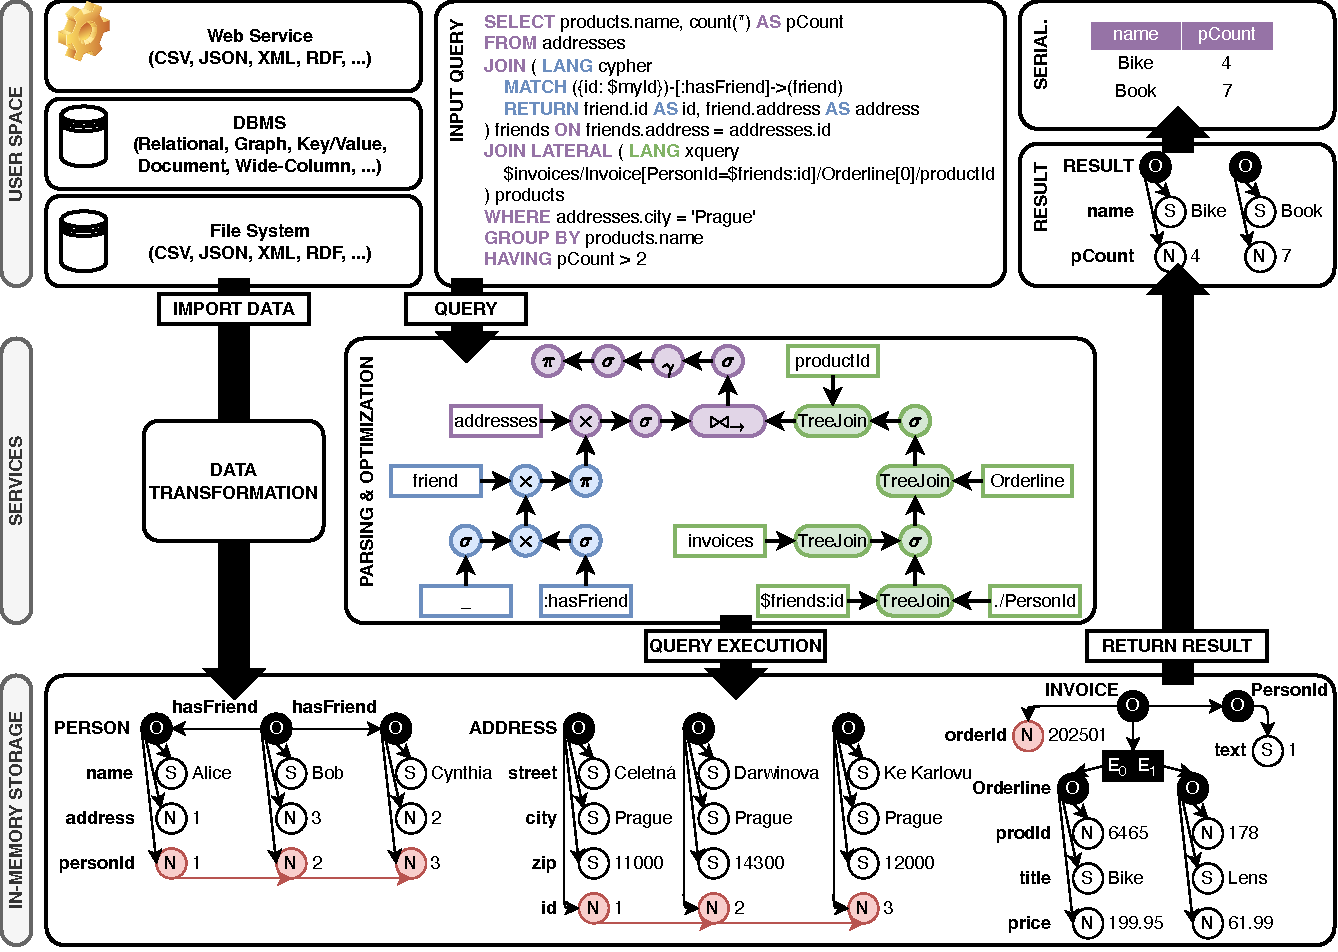
\includegraphics[width=\linewidth]{img/dortDB-workflow.pdf}
    \caption{Data import and query evaluation workflow in DortDB. The diagram was created by Pavel Koupil and comes from a demo paper accepted to the 51\textsuperscript{st} VLDB conference, which the author of this thesis coauthored with Pavel Koupil, Michal Kopecký, Jáchym Bártík, and Irena Holubová, but which has not yet been published at the time of writing.}
\end{figure}

\chapter{Implemented languages}
\label{chap:implemented-langs}

As DortDB aims to support any query language, we have implemented three initial languages, one for each major data model. None of the languages was implemented completely. Given that DortDB does not aim to support data definition and manipulation (at least initially), the languages were trimmed to their data selection subset. Additionally, most of the typing and schema validation features were removed, as they couple the language too tightly with the underlying data representation.

\section{SQL}

SQL (standing for Structured Query Language) is a relational query language based on relational algebra and relational calculus. It became an ISO standard in 1987; the latest version of the standard was published in 2023\cite{sql_iso_2023}. The language operates in terms of tables (relations). Each table has a schema, which consists of a name and a set of attributes. Tables contain rows (tuples), whose values are called columns and correspond to the schema attributes. Important SQL operations include joins of relations and data aggregation.

The DortDB SQL language is based on the PostgreSQL SQL flavor\footnote{\url{https://www.postgresql.org/}}. It also includes several of the PostgreSQL JSON access operators.

\subsection{Notable features}

PostgreSQL includes several features that are not usual in other SQL flavors. Among them belong the following:

\subsubsection*{Lateral joins}

Lateral joins allow joining of correlated subqueries. In other words, it is possible for the joined subquery to refer to previous tables, and thus to be re-evaluated for different outer contexts.

\begin{minted}{sql}
SELECT t1.attr1, s.attr2 FROM t1
JOIN LATERAL (
  SELECT t2.attr2 FROM t2
  -- the WHERE clause refers to the outer context
  -- the subquery is reevaluated for each t1 row
  WHERE t2.attr3 + t1.attr4 > t1.attr5
) AS s
\end{minted}

\subsubsection*{\texttt{DISTINCT ON}}

The \texttt{DISTINCT} modifier filters out duplicate values. PostgreSQL allows customizing this behavior.

\begin{minted}{sql}
SELECT DISTINCT ON (attr1, attr2 % 10) attr1, attr2, attr3
FROM t1
\end{minted}

\subsubsection*{Complex aggregate calls}

The arguments of aggregate calls such as \texttt{count} or \texttt{sum} may be filtered or sorted.

\begin{minted}{sql}
SELECT
  count(DISTINCT attr1) AS distinct_count,
  count(attr1) FILTER (WHERE attr1 % 2 = 0) AS even_count,
  collect(attr1 ORDER BY attr1) AS ordered_array
FROM t1
\end{minted}

\subsection{Schema of data sources}
\label{subsec:sql-schema-data-sources}

SQL expects tables to have a clearly defined schema. This enables users to write queries that would otherwise be ambiguous.

\begin{minted}{sql}
-- which tables are a, b, or c from?
SELECT a, b, c
-- what columns are used in the natural join?
FROM t1 NATURAL JOIN t2
\end{minted}

DortDB data sources are, however, schemaless by design. Therefore, the allowed SQL queries face some restrictions. It must be clear from which tables specific columns originate. Non-qualified column names are only allowed when there is only a single, non-joined data source. Natural joins are disabled. All \texttt{FROM} clause subqueries must have an alias. Selecting all attributes using asterisk \texttt{*} is also disabled, although in theory it should be possible. When an attribute should not be interpreted as belonging to the current table, it should be prefixed by the \texttt{nonlocal} schema. This becomes relevant later, when inserting SQL subqueries into languages that do not prefix identifiers, such as Cypher.

\begin{minted}{sql}
-- t1.attr1
SELECT attr1 FROM t1
-- t2.attr2, t2.attr3, t1.attr1
WHERE (SELECT attr2 FROM t1 WHERE attr3 < nonlocal.attr1)
\end{minted}

To optimize the query plan later, some knowledge about the schema of the data sources and of the individual logical plan operators is necessary. Therefore, all of the referenced attributes must be paired with their data sources to infer their schema. This process happens once the logical plan is built and all of the used attributes are known.

\subsection{Not implemented features}

Besides data types, there are features that are not currently part of the DortDB SQL. The parser recognizes them, but they have not yet been implemented. The functionality will be added sometime in the future. This includes window functions, special \texttt{GROUP BY} features such as \texttt{ROLLUP}, or (possibly recursive) common table expressions.

\section{XQuery}

XQuery\footnote{\url{https://www.w3.org/TR/2014/REC-xquery-30-20140408}} is a functional programming language designed for querying structured and semi-structured XML data. It contains a superset of XPath\footnote{\url{https://www.w3.org/TR/xpath-31/}}, an expression language for querying XML. XPath operates in terms of sequences of values. Sequences cannot be nested; a sequence of sequences is interpreted as if it were flattened. Conversely, the values can be interpreted as sequences with one element. Null values are treated as empty sequences. XQuery adds SQL-like FLWOR expressions, named after some of the available clauses: For, Let, Where, Order by, and Return. Within FLWOR expressions, data is streamed as sequences of named tuples of values, but a FLWOR expression may return only sequences of opaque items. XQuery cannot accept or produce tuples.

\begin{minted}{xquery}
for $x in $source/foo (: $source/foo is an XPath expression :)
let $y := $x/bar (: $y is a sequence :)
(: data is passed between clauses
   as tuples with attributes x and y :)
return $y (: the result of the FLWOR is a flattened sequence :)
\end{minted}

Aggregation in XQuery is done by passing a sequence into a function. For example, summing numbers from 1 to 10 can be done like so:

\mint{xquery}{sum(1 to 10)}

XPath defines an expression's static and dynamic context. The static context consists of information available during the expression's static analysis and contains information such as statically known namespaces or in-scope variables. The dynamic context contains the current context item (referenced by a single dot or by the special variable \texttt{\$fs:dot}), the current context position (referenced by the function \texttt{fn:position()} or by the special variable \texttt{\$fs:position}), and the current context size (referenced by the function \texttt{fn:last()} or by the special variable \texttt{\$fs:last}).

\begin{minted}{xquery}
declare namespace foo = "http://example.org";
(: the static context now includes the foo namespace :)

(5 to 10)[
  (:
  the predicate can access the current item (numbers from 5 to 10),
  the current position (numbers from 1 to 5),
  and the current context size (number 5)
  :)
  . mod 2 eq 1
]
(: the result is the sequence (5,7,9) :)
\end{minted}

DortDB XQuery is a subset of XQuery 3.0.

\subsection{Not implemented features}

The DortDB XQuery implementation does not include any typing except \texttt{cast} expressions. This means that the following is not (and is not ever planned to be) available:

\begin{itemize}
    \item \texttt{as} keyword
    \item \texttt{typeswitch} expressions
    \item \texttt{instance of} expressions
    \item \texttt{treat} expressions
    \item \texttt{instance of} expressions
    \item \texttt{castable} expressions
    \item \texttt{validate} expressions
    \item any function types except \texttt{function(*)} 
    \item function references containing arity information (\texttt{fnname\#arity})
\end{itemize}

The following is also not implemented, but may be added in the future:

\begin{itemize}
    \item \texttt{try catch} expressions
    \item pragma expressions
    \item \texttt{window} FLWOR clause
    \item inline functions
    \item \texttt{\%private} and \texttt{\%public} modifiers
    \item any module prolog except namespace definition
\end{itemize}

\section{Cypher}

Cypher is a declarative graph query language developed for the Neo4j database\footnote{\url{https://neo4j.com/docs/cypher-manual/25/introduction/}}. The DortDB Cypher language is based on openCypher, which is an open source specification of Cypher. Since the release of GQL (Graph Query Language) by ISO\footnote{\url{https://www.iso.org/standard/76120.html}} in April 2024, the aim of the openCypher project is to converge towards GQL and ease the transition of graph databases towards the ISO standard.

Cypher operates on labeled property graphs, a graph data model in which both nodes and relationships may contain properties. Furthermore, nodes may have zero or more labels, while each relationship has exactly one type. Relationships are always directed.

\begin{figure}[ht!]
  \centering
  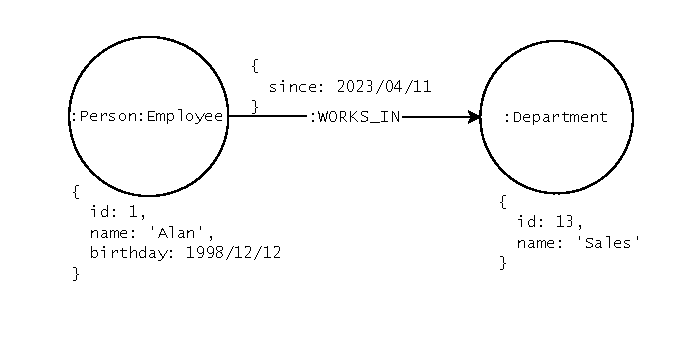
\includegraphics[width=0.7\textwidth]{img/lpg.pdf}
  \caption{Labeled property graph}
  \label{fig:lpg}
\end{figure}

\pagebreak

Cypher provides a visual way of matching patterns and relationships using ASCII art. It is possible to match recursive paths. A matched path cannot contain duplicate relationships, but each node may be visited multiple times.

\begin{minted}{cypher}
    §\textcolor{teal}{\texttt{\textup{//} \textit{match each neighbor of Alan, regardless of direction}}}§
    §\textcolor{teal}{\texttt{\textup{//} \textit{the neighbors will be stored in the 'neighbor' variable}}}§
    MATCH (:Person {name: "Alan"})-[]-(neighbor)

    §\textcolor{teal}{\texttt{\textup{//} \textit{match Alan's friends of friends, up to three hops far,}}}§
    §\textcolor{teal}{\texttt{\textup{//} \textit{and then find their employers}}}§
    §\textcolor{teal}{\texttt{\textup{//} \textit{the p variable will contain a list of relationships}}}§
    MATCH ({name: "Alan"})-[p:KNOWS *1..3]->(foaf)
      <-[:EMPLOYS]-(employer)

    §\textcolor{teal}{\texttt{\textup{//} \textit{the recursive path may match patterns like}}}§
    §\textcolor{teal}{\texttt{\textup{//} \textit{(alan)->(x)->(alan)->(y)}}}§
    §\textcolor{teal}{\texttt{\textup{//} \textit{but it cannot match the same relationship twice}}}§
    §\textcolor{teal}{\texttt{\textup{//} \textit{(alan)->(x)->(alan)->(x)}}}§
\end{minted}

It is then possible to process the matched values similarly to SQL.

\begin{minted}{cypher}
    MATCH (x)-[]->(y)
    WHERE y.age < 15
    RETURN x.name, y.age
    ORDER BY x.name
    SKIP 3
\end{minted}

\subsection{Differences between DortDB and openCypher}

The DortDB Cypher language is parsed with an LALR(1) parser, which is not powerful enough for the original openCypher grammar, as it has only a limited lookahead. The grammar contains constructs that would be ambiguous during parsing. We have, therefore, decided to always parse certain patterns a certain way, even though it means that some otherwise valid queries will fail.

\subsubsection*{Node patterns or parenthesized expressions}

If the input can be interpreted as either the start of a node pattern or a parenthesized expression, the parser will always choose the node pattern.

\begin{itemize}
    \item \texttt{(a)} is a node pattern
    \item \texttt{(a:Label)} is a node pattern
    \item \texttt{(\{prop: value})\} is a node pattern
    \item \texttt{(\$param)} is a node pattern
\end{itemize}

Because of this, \texttt{(a:Label = true)} will cause a parsing error, because it is already considered a node pattern, even though it would be a valid expression in the original grammar, checking whether the \texttt{a} variable has the \texttt{Label} label. The same goes for \texttt{({prop: value}.prop)}. More complex parenthesized expressions starting with a variable or a parameter are not affected, for example, \texttt{(\$param = true)} or \texttt{(a + a)} are valid expressions.

This should not cause any issues, as it is always possible to interpret the input as expressions by removing the parentheses. The label check expression \texttt{a:Label} has the highest precedence, so parentheses would not do anything anyway, and the rest are simply parentheses around atomic expressions.

\subsubsection*{Operators}

The following symbol combinations are considered part of relationship patterns and will not be interpreted as operators. If necessary, it is always possible to clarify the meaning by adding parentheses.

\begin{itemize}
    \item \texttt{<-[} (e.g., it will never be parsed as a comparison like \texttt{a < -[b]})
    \item \texttt{<--}
    \item \texttt{--}
    \item \texttt{-[}
\end{itemize}

\subsubsection*{List/pattern comprehension or list literals}

Cypher includes special syntax for list comprehension and pattern comprehension.

\begin{minted}[ignorelexererrors=true]{cypher}
RETURN [x IN range(0,10) WHERE x % 2 = 0 | x^3] AS result

MATCH (a:Person)
RETURN [(a)-[:KNOWS]->(b) WHERE b:Person | b.name] AS friends

MATCH (a {id: 1})
RETURN [path = (a)-[:KNOWS*]->(b) | size(path)] AS foafDistances
\end{minted}

If the input can be interpreted as either the start of a list/pattern comprehension or a list literal, the parser will always choose the list/pattern comprehension. More specifically, if the input starts with:

\begin{itemize}
    \item \texttt{[variable IN}
    \item \texttt{[variable = (pattern)}
\end{itemize}

Then it is no longer possible to interpret it as a list literal (even though in the original grammar, \texttt{[variable IN list1, variable IN list2]} would be a valid list literal containing two booleans).

\subsubsection*{Reserved words}

In addition to the regular reserved words, the following words need to be escaped before they can be used as identifiers.

\begin{itemize}
    \item \texttt{COUNT}
    \item \texttt{ANY}
    \item \texttt{NONE}
    \item \texttt{SINGLE}
\end{itemize}
\chapter{Multilanguage queries}
\label{chap:multilang-queries}

In DortDB, we want to provide a common framework for queries regardless of the query language. A direct conclusion is to allow mixing languages in a single query. This enables the user to separate their query into logical parts and express each in a language they find the most intuitive. It also offers the possibility to form multimodel queries using the languages initially developed for each model.

Existing implementations of this idea include SQL/XML or OpenLink Virtuoso's SPASQL\cite{virtuoso_spasql}. SQL/XML uses new functions and datatypes, which facilitate queries combining relational and document models, but it is rather verbose. SPASQL, or SPARQL-in-SQL, allows for embedding SPARQL subqueries into SQL. However, it is not possible to embed SQL subqueries into SPARQL.

\section{Language switching}
\begin{comment}
- dict X single value
- arango db: forin
- orient db: no join
- spasql: rel X rel

Algebra:

- https://ieeexplore.ieee.org/abstract/document/1617382 (xquery)
- https://ieeexplore.ieee.org/abstract/document/1410186 (xpath)
- Optimization of Nested Queries using the NF2 Algebra
- Handling Environments in a Nested Relational Algebra
with Combinators and an Implementation in a Verified
Query Compiler
- SQL query optimization through nested relational algebra
- The relational model with relation-valued attributes
- https://arxiv.org/pdf/2407.04823
- https://arxiv.org/pdf/1908.06265v1
- https://drops.dagstuhl.de/storage/00lipics/lipics-vol098-icdt2018/LIPIcs.ICDT.2018.9/LIPIcs.ICDT.2018.9.pdf
- https://cseweb.ucsd.edu/classes/wi20/cse232B-a/papers/staircase.pdf
\end{comment}

Our approach extrapolates on SPASQL to allow embedding any language subqueries into any language. It is necessary to establish clear rules for the language-to-language interfaces. In some cases, the transition is intuitive -- e.g., a SQL query that selects attributes from a Cypher subquery. The Cypher subquery returns a set of tuples, just like a SQL subquery would. On the other hand, SQL might sometimes require the subquery only to produce a single value. Some languages do not operate in terms of tuples, such as XPath. Our solution is to separate the subqueries into those producing tuples and those producing opaque items. Each language is then responsible for converting the results of these subqueries as necessary.

\begin{listing}[!ht]
\begin{minted}{sql}
SELECT attr1, attr2 FROM (
  -- subquery
);

SELECT (SELECT count(*) FROM table1) AS total, count(*)
FROM table1
GROUP BY item_id;
\end{minted}
\caption{Example of two SQL subqueries. The first subquery produces tuples, the second produces only a single value.}
\end{listing}

The language switch subqueries are demarcated by the \texttt{LANG} keyword on one side and either by a scope exit (a closing bracket or parenthesis) or by the \texttt{LANG EXIT} keywords on the other. The nested language can use variables available in the parent scope. In case of languages such as SQL, the attributes used by the nested language are used to infer the schema of referenced relations.

\begin{listing}[!ht]
\begin{minted}{sql}
SELECT id, ARRAY(
  LANG cypher
\end{minted}
\nestedMintedVspace
\begin{minted}[style=manni]{cypher}
  MATCH (:person {id: people.id})-[:KNOWS]->(friend)
  RETURN friend
\end{minted}
\nestedMintedVspace
\begin{minted}{sql}
) AS friends
FROM people
\end{minted}
\caption{Cypher nested into SQL refers to the outer relation \texttt{people}.}
\end{listing}

\begin{figure}[htpb]
    \begin{subfigure}[b]{\textwidth}
    \begin{tcolorbox}[colback=white, colframe=black, boxrule=1pt, arc=0pt]
        \begin{minted}[fontsize=\small]{sql}
SELECT foo.frst, (
  LANG xquery
        \end{minted}
        \nestedMintedVspace
        \begin{minted}[style=manni,fontsize=\small]{xquery}
  for $x in $xs
  return $foo:second + (
        \end{minted}
        \nestedMintedVspace
        \begin{minted}[fontsize=\small]{sql}
    LANG §\texttt{sql}§
    SELECT foo.third FROM bar
  )
) AS nested
FROM foo
        \end{minted}
    \end{tcolorbox}
    \end{subfigure}
    
    \medskip
    
    \begin{subfigure}[b]{\textwidth}
        \centering
        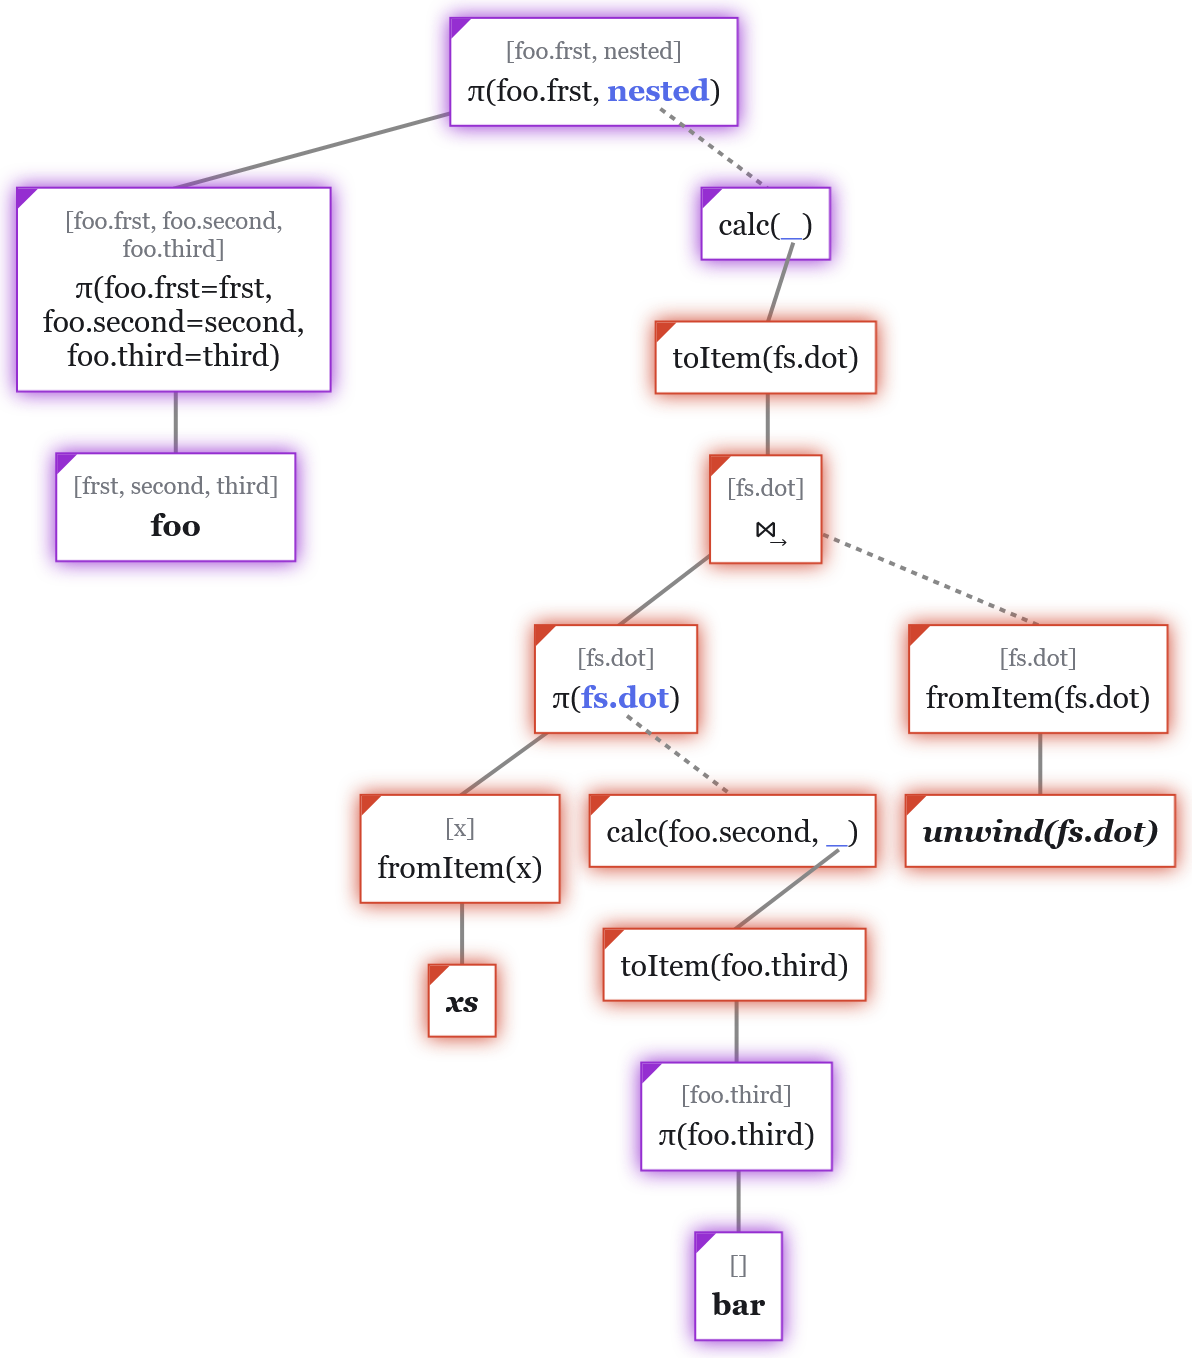
\includegraphics[width=360pt]{img/tree-sql-infer.png}
    \end{subfigure}
    
    \caption{The SQL parser can use information from the nested languages to infer the schema of the \texttt{foo} relation. The logical operator tree is partially optimized for better readability. Diagrams like this are explained in section \ref{sec:algebra}. For now, the important thing is that the grey brackets in some nodes denote the tuple schema of the corresponding operator.}
\end{figure}

\section{Unified algebra}
\label{sec:algebra}

Queries are parsed into a logical operator tree, where each node corresponds to an operator from \textit{unified algebra}. The unified algebra covers most of the expected query operations. It is, however, possible for any language to extend the algebra and to define its own operators. This way, it is possible to cover any future languages regardless of their model. This process is more closely explained in section \ref{sec:usage-extensibility}.
%\hl{/*KOP je/bude nekde popsane, jak to udelat? (Cestina s hacky a carkami se v PDF spatne renderuje, tak budu psat komentare bez nich.)*/}

%\hl{/*KOP z ciste estetickeho hlediska bych psal vsechny LANG jednotne velkymi pismeny. V obrazku je LANG xquery, ale lang sql.*/}

The algebra is based on algebras for XQuery\cite{xquery_algebra}, graph paths\cite{angles2024path} and nested relational algebra\cite{schek1986relational}. We divide the operators into two main groups. \textit{Tuple operators} operate on streams of named tuples, similarly to relational algebra. \textit{Item operators} operate on streams of opaque items. Depending on their arguments, some operators may be considered either item or tuple operators. One such example is the \texttt{limit} operator.

\begin{longtable}{|>{\raggedright\arraybackslash}p{5cm}|>{\raggedright\arraybackslash}p{9cm}|}
\hline
\textbf{Algebraic Operator} & \textbf{Operator's Signature} \\ 
\hline
\endfirsthead
\hline
\textbf{Algebraic Operator} & \textbf{Operator's Signature} \\ 
\hline
\endhead
\hline
\endfoot

\multicolumn{2}{|c|}{\textbf{Item Operators}} \\ 
\hline
\textbf{Calculation Intermediaries} & \\
AggregateCall & $\text{agg}(\texttt{args})$ \\
Conditional & $\text{cond}(\texttt{expr}, \texttt{whenthens}, \texttt{default})$ \\
FnCall & $\text{fn}(\texttt{args})$ \\
Literal & $\text{literal}(\texttt{value})$ \\
Quantifier & $\text{quant}(\texttt{type}, \texttt{query})$ \\
\hline
\textbf{Other} & \\
Calculation & $\text{calc}(\texttt{args})$ \\
ItemSource & $\textit{name}$ \\
ItemFnSource & $\textit{name}(\texttt{params})$ \\
MapToItem & $\text{toItem}(\texttt{key}, \texttt{source})$ \\
\hline
\multicolumn{2}{|c|}{\textbf{Tuple Operators}} \\ 
\hline
\textbf{SPJ} & \\
CartesianProduct & $\times(\texttt{left},\texttt{right})$ \\
Join & $\bowtie(\texttt{left},\texttt{right},$ $\texttt{leftOuter},\texttt{rightOuter},\texttt{conditions})$ \\
Projection & $\pi(\texttt{attrs},\texttt{source})$ \\
ProjectionConcat & $\stackrel{\bowtie}{\rightarrow}(\texttt{mapping}, \texttt{outer}, \texttt{source})$ \\
ProjectionIndex & $\text{index}(\texttt{name}, \texttt{source})$ \\
Selection & $\sigma(\texttt{expression}, \texttt{source})$ \\
\hline
\textbf{Other} & \\
Distinct & $\delta(\texttt{attributes}, \texttt{source})$ \\
GroupBy & $\gamma(\texttt{keys},\texttt{aggs},\texttt{source})$ \\
MapFromItem & $\text{fromItem}(\texttt{key}, \texttt{source}) $ \\
OrderBy & $\tau(\texttt{orders},\texttt{source})$ \\
Recursion & $\phi(\texttt{min}, \texttt{max}, \texttt{condition}, \texttt{source})$ \\
TupleSource & $\textbf{name}$ \\
TupleFnSource & $\textbf{name}(\texttt{params})$ \\
\hline
\textbf{XQuery} & \\
ProjectionSize & $\text{size}(\texttt{name}, \texttt{source})$ \\
TreeJoin & $\text{treeJoin}(\texttt{expr}, \texttt{source})$ \\
\hline
\textbf{Optimizer} & \\
IndexScan & $\textbf{indexScan}(\texttt{name}, \texttt{access})$ \\
IndexedRecursion & $\stackrel{\phi}{\rightarrow}(\texttt{min}, \texttt{max}, \texttt{mapping}, \texttt{source})$ \\
\hline
\multicolumn{2}{|c|}{\textbf{Universal Operators}} \\ 
\hline
NullSource & $\square$ \\
Limit & $\text{limit}(\texttt{skip}, \texttt{limit})$ \\
\hline
\textbf{Set} & \\
Difference & $\setminus(\texttt{left}, \texttt{right})$ \\
Intersection & $\cap(\texttt{left}, \texttt{right})$ \\
Union & $\cup(\texttt{left}, \texttt{right})$ \\
\hline

\end{longtable}

\subsection{Visualization}

The DortDB GUI includes visualization of query plans. The plans are visualized as a tree where each node corresponds to an operator. The tree's root is the final query; the leaves are individual data sources. Each node is colored based on the language it originated from. Tuple operator nodes include the operator schema. The edges are either a solid or a dashed line. Solid edges mean that the child operator is created only once at the same time as its parent. Dashed edges indicate a child operator that is dynamically recreated multiple times during its parent's lifetime.

The source code of the GUI is available as an appendix to this work. The GUI is also available online at \url{https://filipjezek.github.io/dortdb}. The reader is encouraged to try things out for themselves.

\begin{figure}[htpb]
    \begin{subfigure}[b]{\textwidth}
    \begin{tcolorbox}[colback=white, colframe=black, boxrule=1pt, arc=0pt]
        \begin{minted}[fontsize=\small]{sql}
SELECT x + 3 AS xplusthree FROM table1
        \end{minted}
    \end{tcolorbox}
    \end{subfigure}
    
    \medskip
    
    \begin{subfigure}[b]{\textwidth}
        \centering
        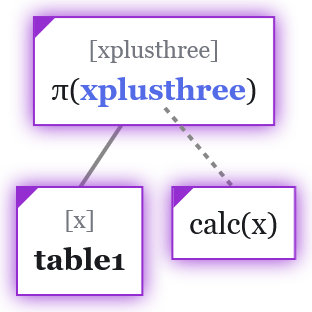
\includegraphics[width=90pt]{img/tree-edge-types.png}
    \end{subfigure}
    
    \caption{The different edge types: \texttt{tupleSource} \textbf{table1} is created once while the \texttt{calculation} is reevaluated for each source row. The \texttt{calculation} edge points directly to its blue representative attribute.}
\end{figure}

\subsection{Operators}

Most of the item operators are calculation intermediaries. They do not participate in the final query plan. Instead, they serve as building blocks for the \texttt{calculation} operator. The \texttt{calculation} operator represents any calculated value, such as \texttt{projection} attributes or \texttt{selection} condition. The \texttt{calculation} arguments can be either attribute identifiers or other (non-calculation-intermediate) plan operators. It is possible to express subqueries using a \texttt{calculation} with e.g. a \texttt{projection} as its argument. In such cases, the \texttt{calculation} tracks whether the subquery is supposed to produce at most one or multiple values. The \texttt{quantifier} operator represents a SQL-style quantified query, for example \mintinline{sql}{x > ALL(SELECT y FROM t)}. The \texttt{aggregateCall} operator represents the result of an aggregation applied to an earlier \texttt{groupBy} operator.

\begin{figure}[htpb]
    \begin{subfigure}[b]{\textwidth}
    \begin{tcolorbox}[colback=white, colframe=black, boxrule=1pt, arc=0pt]
        \begin{minted}[fontsize=\small]{sql}
SELECT x FROM table1
WHERE x < (
  SELECT y FROM table2
)
        \end{minted}
    \end{tcolorbox}
    \end{subfigure}
    
    \medskip
    
    \begin{subfigure}[b]{\textwidth}
        \centering
        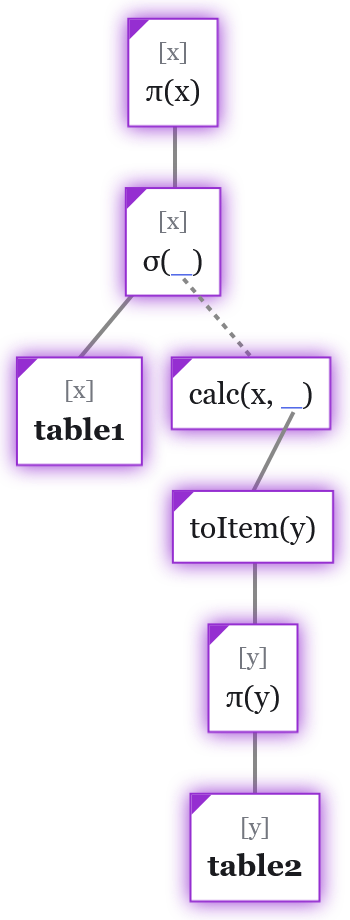
\includegraphics[width=100pt]{img/tree-naive-subquery.png}
    \end{subfigure}
    
    \caption{A subquery can be expressed as a \texttt{calculation} with a \texttt{projection} as an argument.}
    \label{fig:naive-subquery}
\end{figure}

The rest of the full-fledged item operators are data sources, and the \texttt{mapToItem} operator converts tuples to items. It selects the \texttt{key} attribute from each tuple. If the \texttt{key} is the \textit{allAttrs symbol *}, the whole tuple is treated as the new item.

Tuple operators include the well-known \texttt{selection}, \texttt{projection}, \texttt{join}, \\\texttt{cartesianProduct}, and \texttt{orderBy}. \texttt{Join} may include multiple conditions, in which case they must all be satisfied for the two source tuples to be joined. Multiple separated conditions make it easier for the optimizer to recognize certain opportunities. It is also possible to not specify any condition at all and to use the \texttt{join} operator solely for its \texttt{leftOuter} or \texttt{rightOuter} properties.

\texttt{ProjectionIndex} adds a new attribute to each tuple that tracks its ordinal number. \texttt{ProjectionConcat} could be also called \texttt{depend-join}. It is similar to \texttt{join}, in that it joins \texttt{source} tuples to \texttt{mapping} tuples. For each \texttt{source} tuple, the \texttt{mapping} stream is reevaluated, and each of its tuples is joined to the \texttt{source} tuple. The \texttt{mapping} may depend on the context of the \texttt{source} stream. In terms of SQL, the \texttt{projectionConcat} operator can be utilized in correlated subqueries in the \texttt{SELECT} or \texttt{WHERE} clause, or in \texttt{LATERAL JOIN}.

\begin{figure}[htpb]
    \begin{subfigure}[b]{\textwidth}
    \begin{tcolorbox}[colback=white, colframe=black, boxrule=1pt, arc=0pt]
        \begin{minted}[fontsize=\small]{sql}
SELECT x FROM table1
WHERE x < (
  SELECT y FROM table2
)
        \end{minted}
    \end{tcolorbox}
    \end{subfigure}
    
    \medskip
    
    \begin{subfigure}[b]{\textwidth}
        \centering
        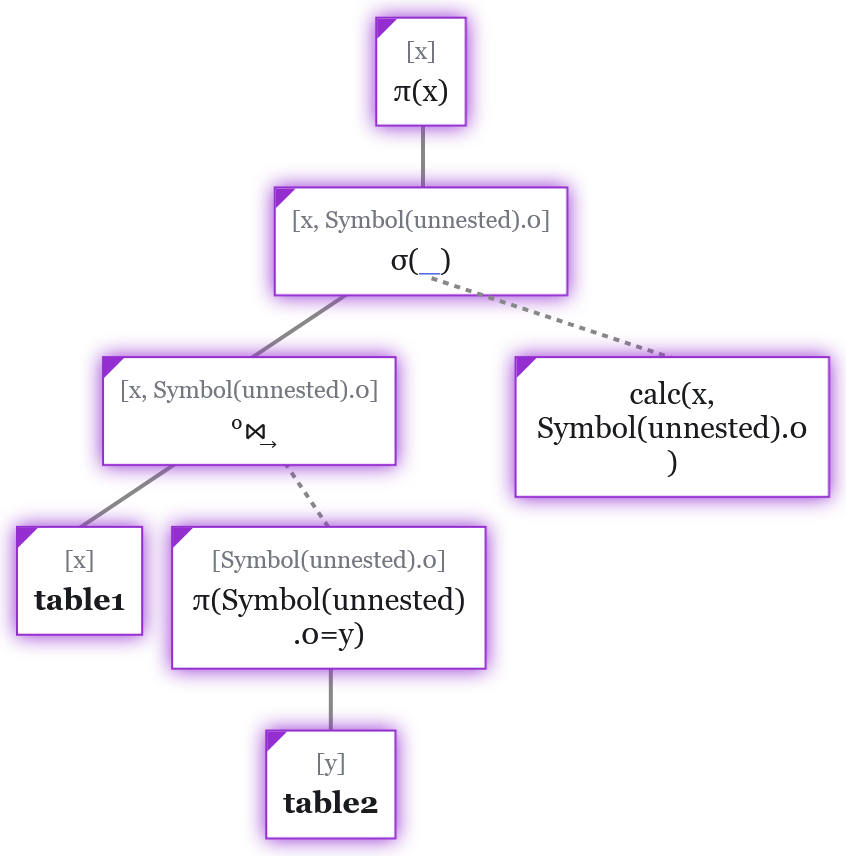
\includegraphics[width=220pt]{img/tree-projconcat-subquery.png}
    \end{subfigure}
    
    \caption{The same query as in figure \ref{fig:naive-subquery}, but the optimizer converted the nested \texttt{projection} to an outer \texttt{projectionConcat}. Note that this is not yet fully optimized. Because the nested \texttt{projection} does not depend on \textbf{table1} context, the \texttt{projectionConcat} can be further converted to a left \texttt{join}.}
\end{figure}

The \texttt{distinct} operator filters out duplicate tuples. The duplicates are decided based on \texttt{attributes}. Similarly to \texttt{mapToItem}, \texttt{attributes} may be the \textit{allAttrs symbol *}. The \texttt{mapFromItem} operator converts an item to a tuple with one attribute named \texttt{key}, which contains the original item. It is not possible to interpret the original item as a tuple.

\texttt{GroupBy} groups \texttt{source} values into partitions based on \texttt{keys}. Each partition is then processed by \texttt{aggregateCall} operators in \texttt{aggs}. Each \texttt{aggregateCall} may contain additional operators that preprocess the partition stream before it is aggregated, for example, when the aggregate requires certain ordering or filtering.

\begin{figure}[htpb]
    \begin{subfigure}[b]{\textwidth}
    \begin{tcolorbox}[colback=white, colframe=black, boxrule=1pt, arc=0pt]
        \begin{minted}[fontsize=\small]{sql}
SELECT
  count(id) FILTER (WHERE sex = 'M') AS men,
  count(id) FILTER (WHERE sex = 'F') AS women,
  collect(DISTINCT id ORDER BY id) AS all_ids
FROM sales
GROUP BY brand
        \end{minted}
    \end{tcolorbox}
    \end{subfigure}
    
    \medskip
    
    \begin{subfigure}[b]{\textwidth}
        \centering
        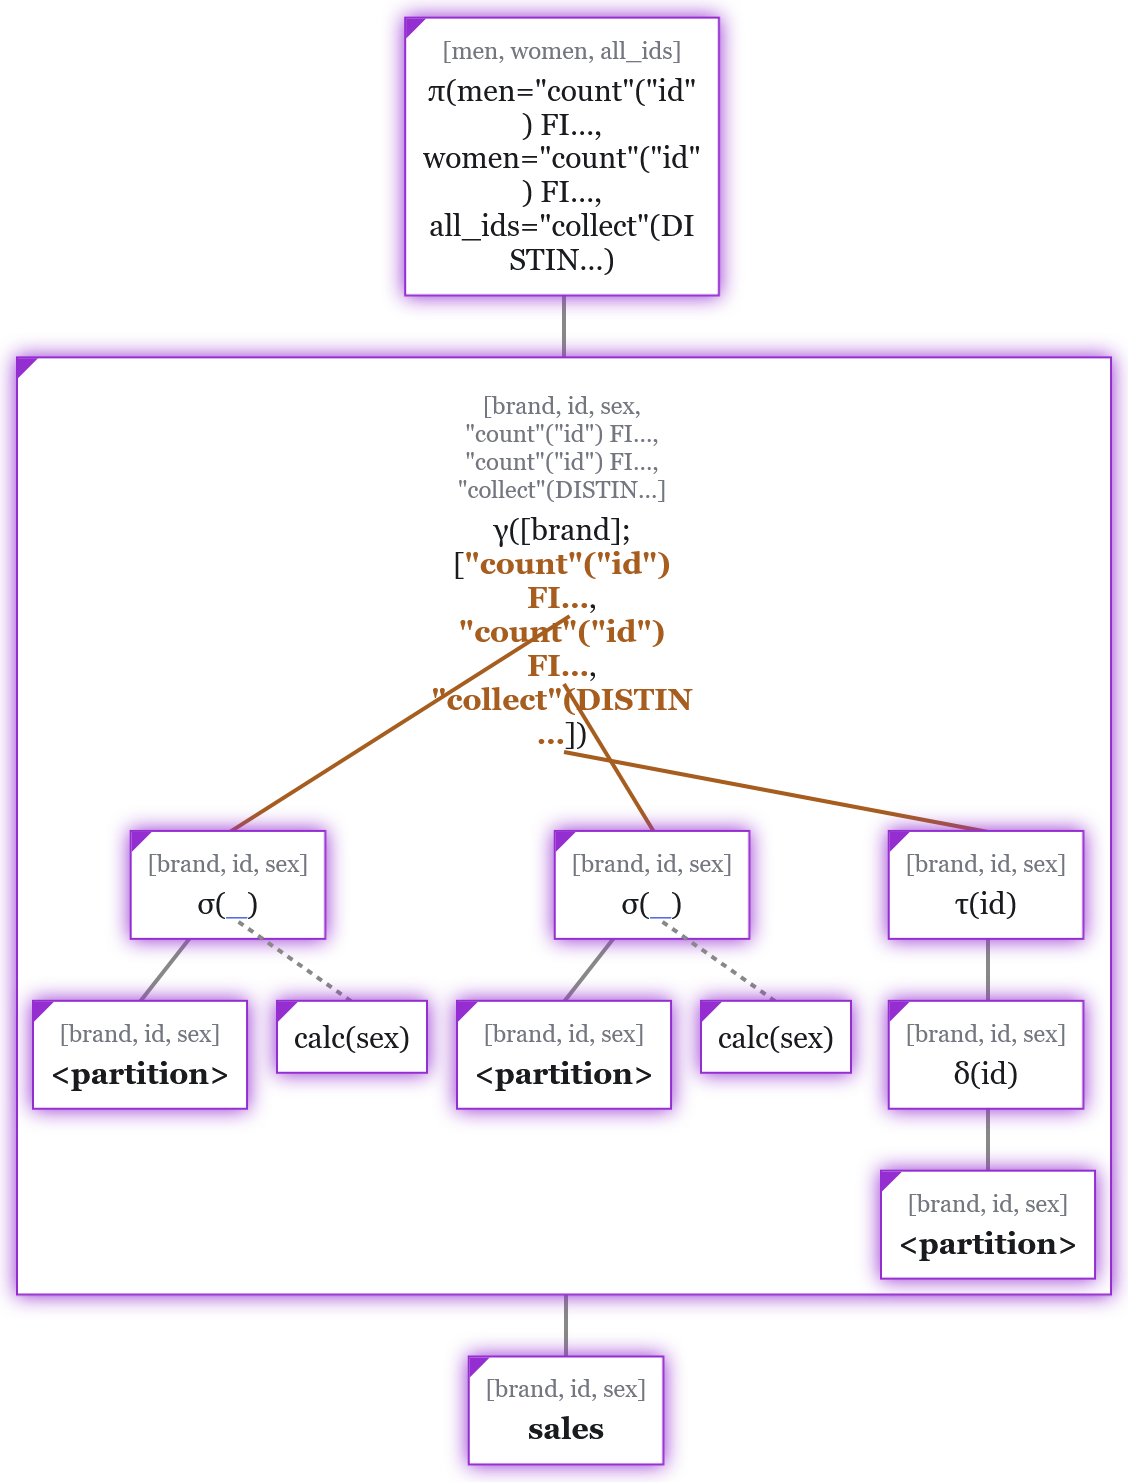
\includegraphics[width=380pt]{img/tree-groupby.png}
    \end{subfigure}
    
    \caption{Example of a complex SQL aggregation. The \texttt{FILTER} clause is defined in SQL:2003 as an optional feature. It is implemented in PostgreSQL and SQLite.}
\end{figure}

The \texttt{Recursion} operator is a self-join repeated up to \texttt{max} times. Its \texttt{condition} can access each \texttt{source} attribute as a pair of an array of accumulated values and the potential next value. The query executor is required to execute the recursion using breadth-first search, so that the shortest values are generated first.

\pagebreak

In order to properly apply indices, there are two specialized operators. \texttt{Index\-Scan} replaces a \texttt{tupleSource} or an \texttt{itemSource} paired with a \texttt{mapFromItem}. It contains an \texttt{access} \texttt{calculation}, which selects relevant items from the underlying data source. The self-join implementation of \texttt{recursion} does not leave any opportunity for indices, so it may be more efficient to use the \texttt{indexedRecursion} operator, which acts as a self-depend-join.

Among the universal operators, which can process both tuples and items, belong the classic set operators like \texttt{union}, \texttt{intersection}, and \texttt{difference}. The \texttt{limit} operator allows only a set amount of results. \texttt{NullSource} is a data source that emits only one empty item.

\begin{figure}[htpb]
    \begin{subfigure}[b]{\textwidth}
    \begin{tcolorbox}[colback=white, colframe=black, boxrule=1pt, arc=0pt]
        \begin{minted}[fontsize=\small]{sql}
SELECT 1 AS one
        \end{minted}
    \end{tcolorbox}
    \end{subfigure}
    
    \medskip
    
    \begin{subfigure}[b]{\textwidth}
        \centering
        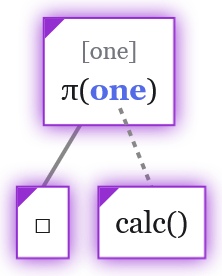
\includegraphics[width=70pt]{img/tree-null-source.png}
    \end{subfigure}
    
    \caption{One possible application for the \texttt{nullSource} operator.}
\end{figure}

Finally, there are two operators used only by XQuery. The \texttt{projectionSize} operator adds a new attribute to each tuple that contains the cardinality of the tuple stream. \texttt{TreeJoin} is a utility operator, which combines \texttt{projectionConcat}, \texttt{projectionIndex} and \texttt{projectionSize}. It is used for path steps like \mintinline{xquery}{a/b/c}. For each step in the path, XQuery must provide a context containing the current item, its position, and the total item count. One notable difference between \texttt{treeStep} and \texttt{projectionConcat} is that \texttt{expr} is a \texttt{calculation} instead of a tuple operator.

\begin{figure}[htpb]
    \begin{subfigure}[b]{\textwidth}
    \begin{tcolorbox}[colback=white, colframe=black, boxrule=1pt, arc=0pt]
        \begin{minted}[fontsize=\small]{cypher}
MATCH ()-[path *2]->()
RETURN path
        \end{minted}
    \end{tcolorbox}
    \end{subfigure}

    \medskip
    
    \begin{subfigure}{\textwidth}
        \centering
        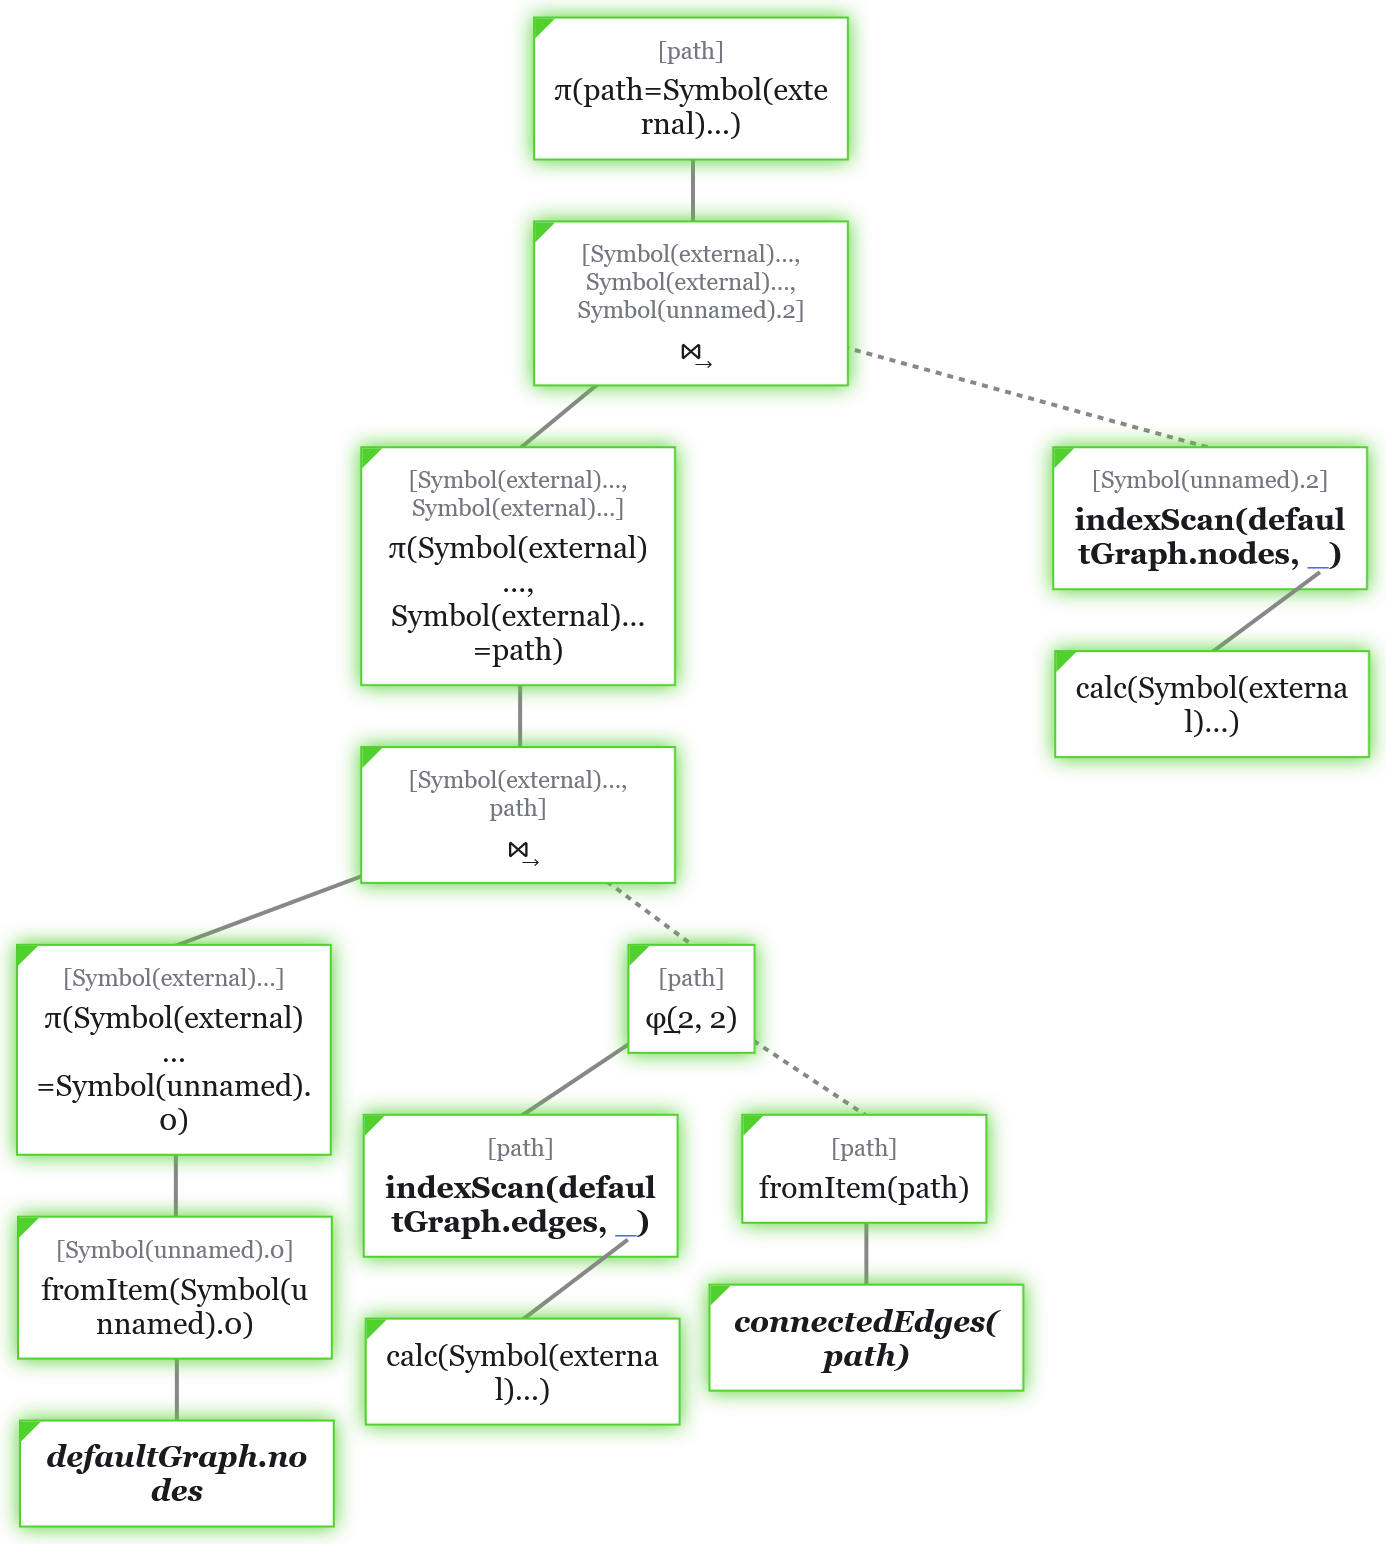
\includegraphics[width=\textwidth]{img/tree-indexed-recursion.png}
    \end{subfigure}
    
    \caption{This cypher query first selects all nodes from a graph. It then selects all of their outgoing edges using an \texttt{indexScan}. These edges are recursively expanded into two-segment paths with the \texttt{indexedRecursion} operator. Finally, another \texttt{indexScan} selects the end nodes of the paths.}
    \label{fig:tree-indexed-recursion}
\end{figure}
\chapter{Optimization}
\label{chap:optimization}

One benefit of having a unified algebra for all languages is that a query can be optimized holistically, regardless of which languages it is written in. DortDB comes with a rule-based optimizer; it is also possible to define secondary indices. Even though cost-based optimizers generally perform better, they require statistics about the queried data. DortDB data sources are, by design, schema-less, and no statistics collection takes place. The optimizer thus consists of an extensible set of query rewriting and operator reordering rules.

\section{Secondary indices}
\label{sec:indices}

Unlike single-model databases, multimodel database systems generally require a broader range of index types\cite{mihal2023refining}. As DortDB aims to be extensible and support as many query languages and models as possible, it is necessary to allow the definition of custom index types. Furthermore, different index types might require different conditions to be applied. For example, a hash table index generally requires the query to contain an equality check on a specific attribute, while a range index can also be applied to inequality comparisons. Our solution is to allow the indexing of any expression composed of \texttt{calculation} intermediaries. This means that any \texttt{calculation} that does not contain subqueries is indexable. During the query optimization phase, registered indices receive expressions used to access a data structure and decide whether they are applicable. Currently, the first matching index is selected. This behavior is contained in two replaceable optimizer rules, so developers using DortDB may implement a better algorithm. In figure \ref{fig:tree-indexed-recursion}, an index provided by the Cypher language detects conditions for connected nodes and edges. In figure \ref{fig:tree-index-scan}, a simple hash table index recognizes a relevant equality check.

\begin{figure}[htpb]
    \begin{subfigure}[b]{\textwidth}
    \begin{tcolorbox}[colback=white, colframe=black, boxrule=1pt, arc=0pt]
        \begin{minted}[fontsize=\small]{ts}
// DortDB programmatic configuration:
this.db.createIndex(['t2'], ['a + b / 2'], MapIndex)
        \end{minted}
    \end{tcolorbox}
    \end{subfigure}

    \begin{subfigure}[b]{\textwidth}
    \begin{tcolorbox}[colback=white, colframe=black, boxrule=1pt, arc=0pt]
        \begin{minted}[fontsize=\small]{sql}
SELECT t1.foo, t2.bar FROM t1
JOIN t2
ON t2.a + t2.b / 2 = t1.id
        \end{minted}
    \end{tcolorbox}
    \end{subfigure}

    \medskip

    \begin{subfigure}[c]{248pt}
        \centering
        \frame{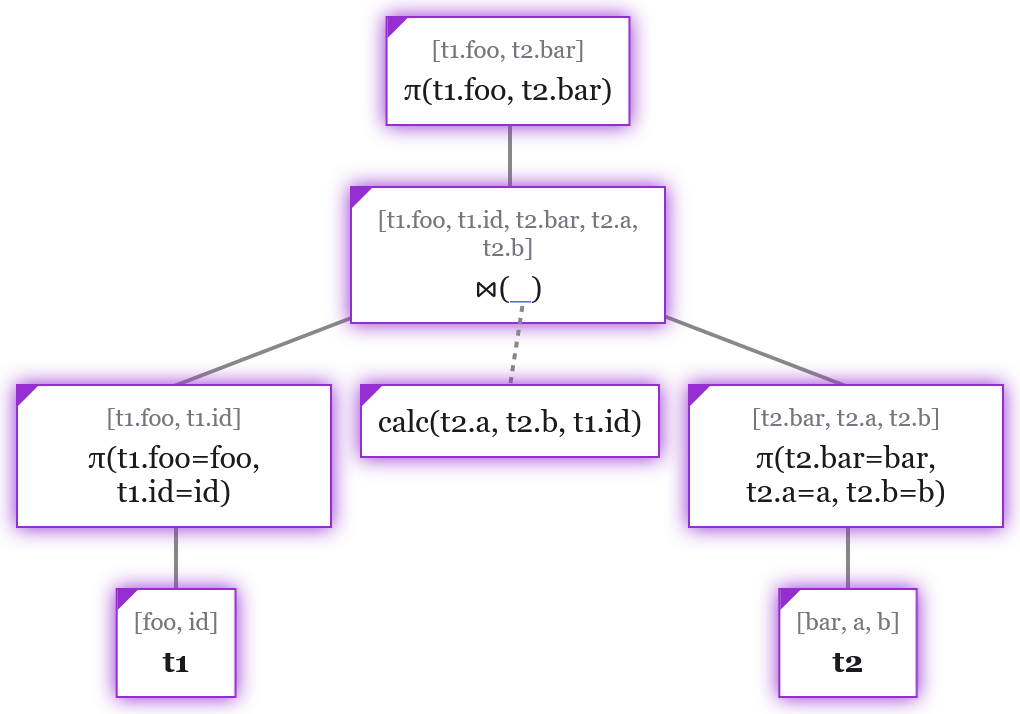
\includegraphics[width=\textwidth]{img/tree-index-scan-before.png}}
    \end{subfigure}\hfill\begin{subfigure}[c]{160pt}
        \centering
        \frame{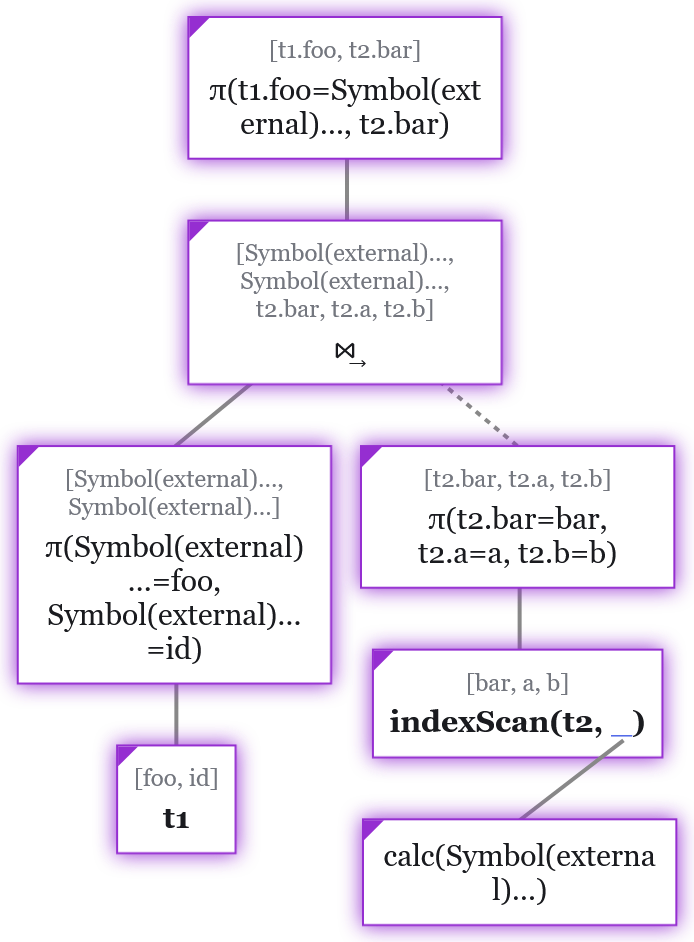
\includegraphics[width=\textwidth]{img/tree-index-scan-after.png}}
    \end{subfigure}
    
    \caption{The registered index recognizes the equality check on the expression it was registered with. Plan before and after the optimization.}
    \label{fig:tree-index-scan}
\end{figure}

\section{Implemented optimizer rules}
\label{sec:optimizer}

The rules in the optimizer follow a simple format. Each rule specifies a set of starting operators. As the rule is processed, the optimizer traverses the query tree from the root down, looking for any operator of a matching type. After such an operator is found, the rule evaluates its \texttt{match} method. If successful, the \texttt{match} function produces bindings, which are supplied to the rule's \texttt{transform} method alongside the subtree starting with the matched operator. The \texttt{transform} method then performs any query rewriting or operator reordering necessary and returns a new subtree, which then replaces the original one.

DortDB comes with a set of implemented rules. During configuration, the user can choose which rules will be used and in what order. In the following sections, the rules will be explained in the order they are applied by default.

\begin{figure}[htpb]
    \begin{subfigure}[b]{\textwidth}
    \begin{tcolorbox}[colback=white, colframe=black, boxrule=1pt, arc=0pt]
        \begin{minted}[fontsize=\small]{sql}
SELECT products.name
FROM products
JOIN (
  LANG cypher
        \end{minted}
        \nestedMintedVspace
        \begin{minted}[style=manni,fontsize=\small]{cypher}
  MATCH (p:person)-[:HAS_INTEREST]->(c:category)
  RETURN p, c.name AS category
        \end{minted}
        \nestedMintedVspace
        \begin{minted}[fontsize=\small]{sql}
) AS interests
ON products.category = interests.category
WHERE interests.p->'id' IN (
  LANG XQuery
        \end{minted}
        \nestedMintedVspace
        \begin{minted}[style=manni,fontsize=\small]{xquery}
  $Invoices/Invoice[
    orderDate < date:sub(now(), interval('1 month'))
  ]/personId/fn:data()
)

        \end{minted}
    \end{tcolorbox}
    \end{subfigure}

    \medskip
    
    \begin{subfigure}{\textwidth}
        \centering
        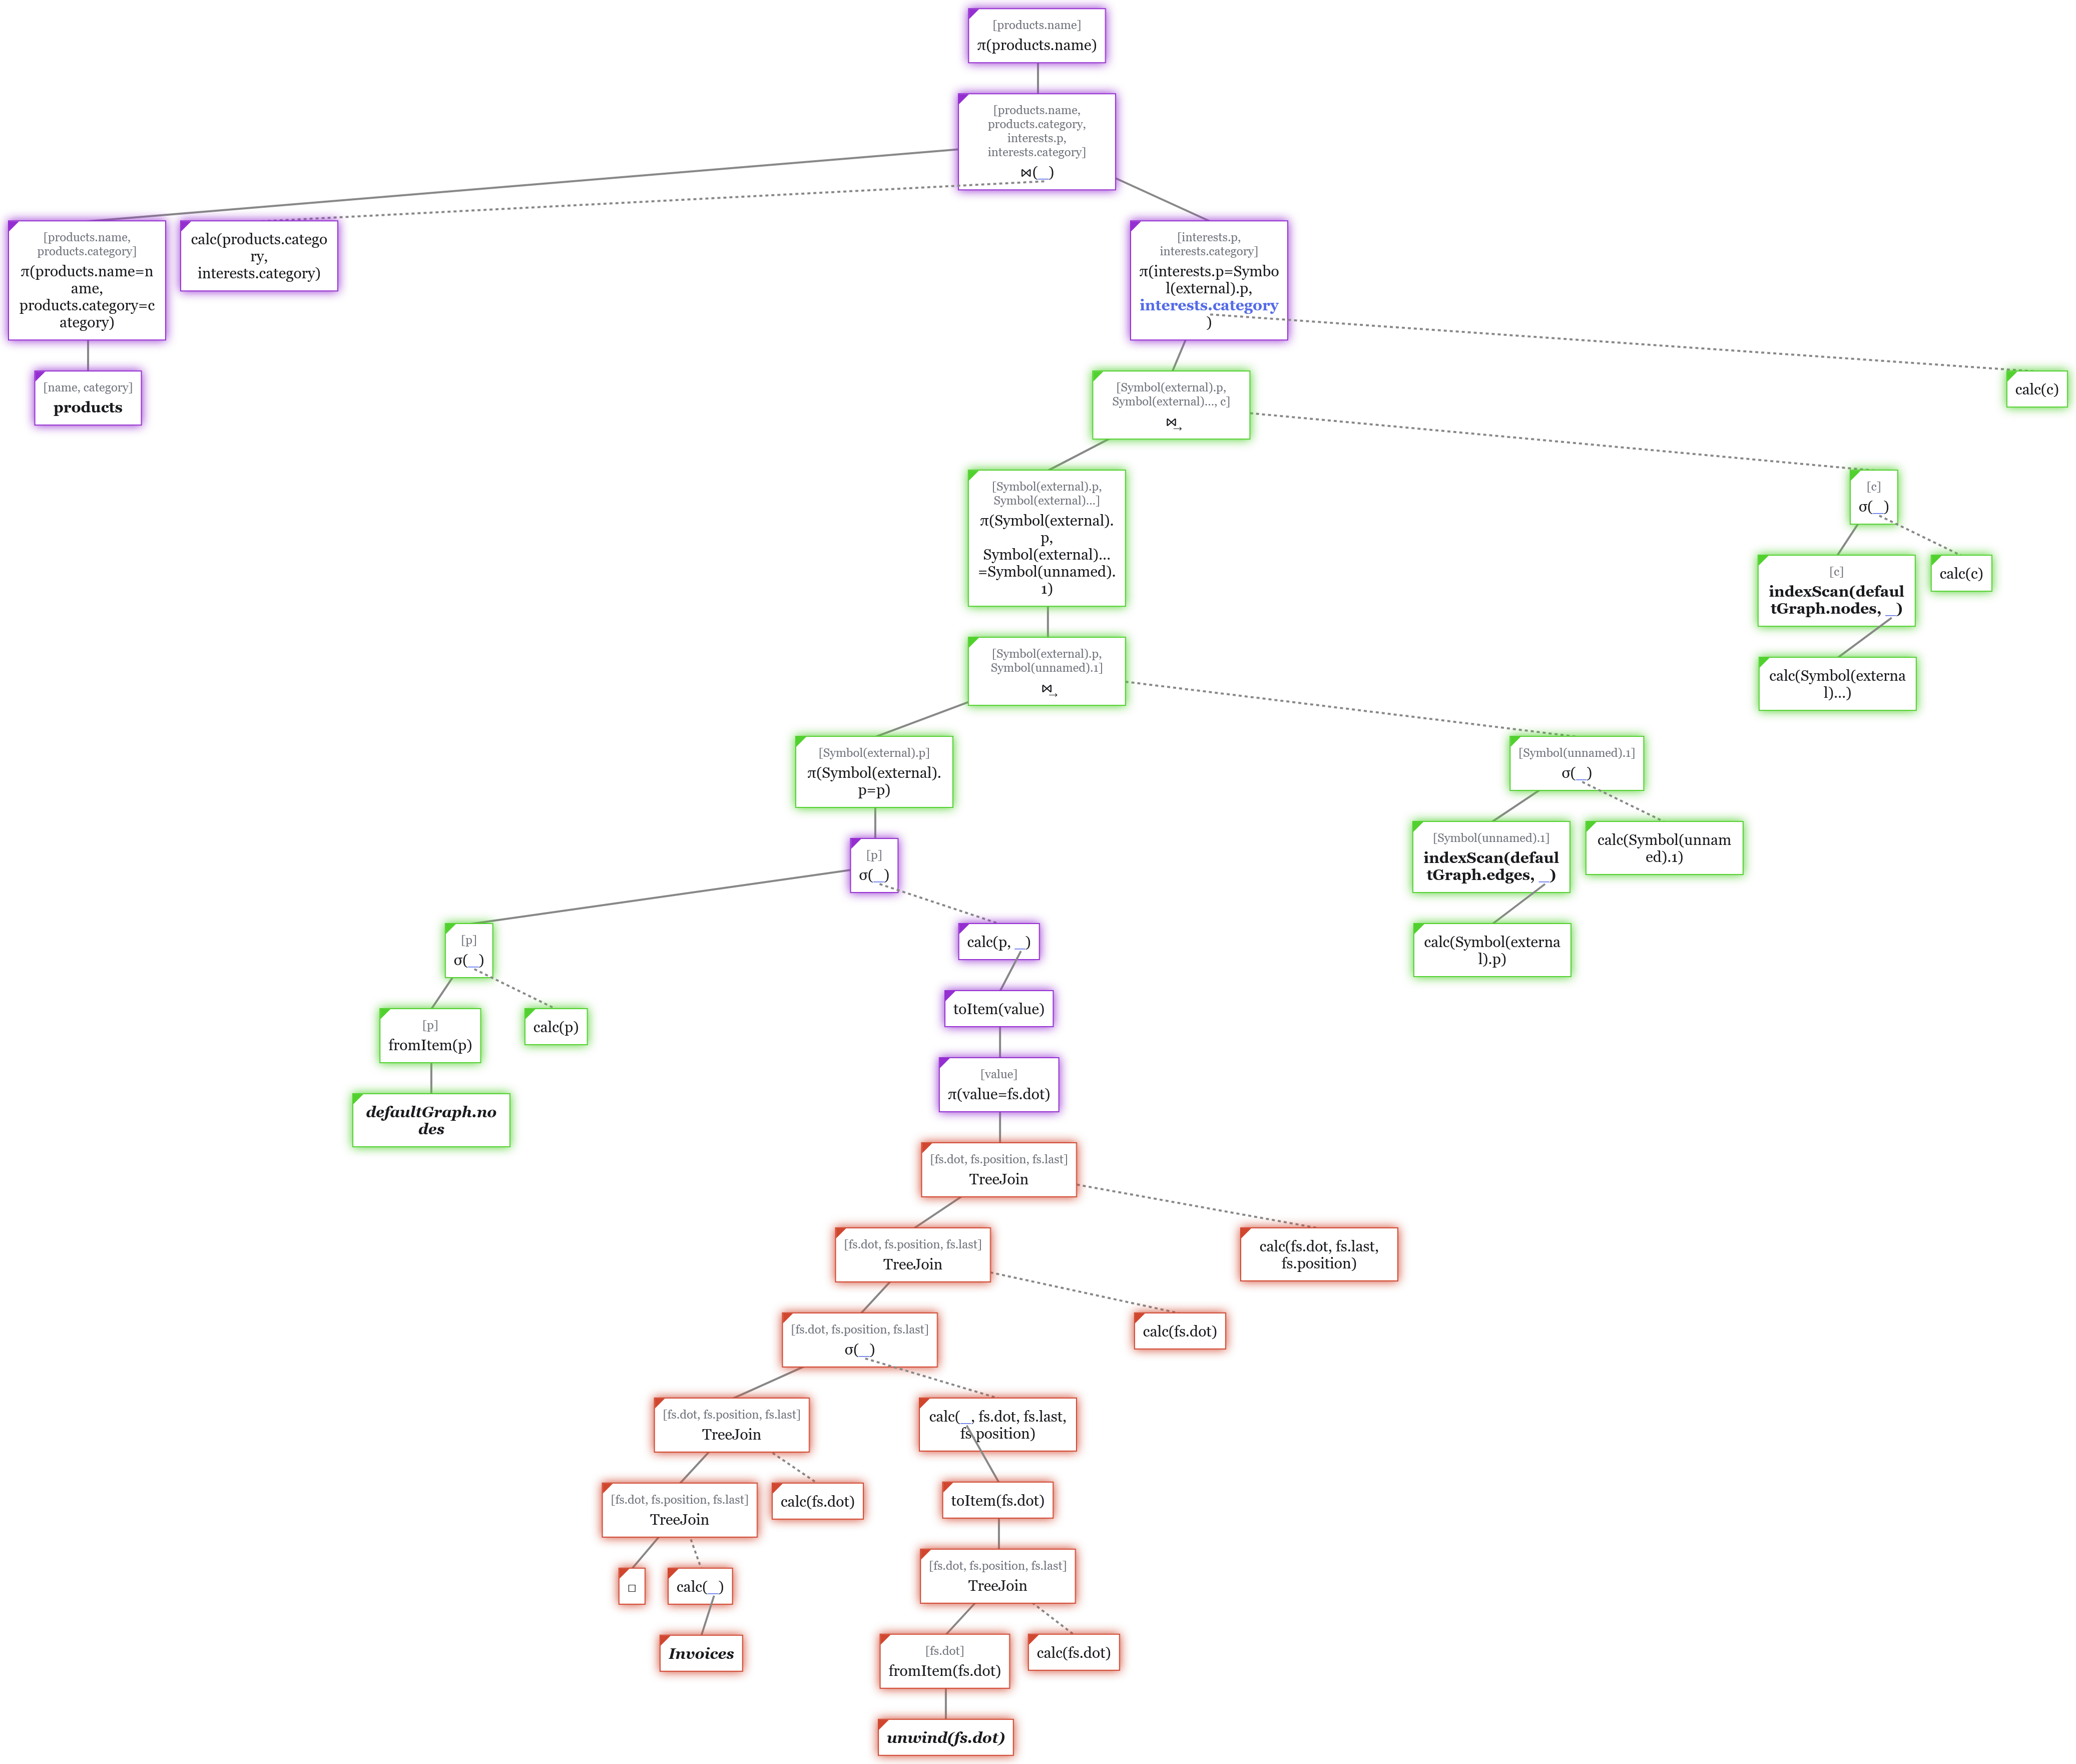
\includegraphics[width=\textwidth]{img/tree-multimodel-optimization.png}
    \end{subfigure}
    
    \caption{Example of how the optimizer works through all the languages at once. Notice the orange-purple subtree, which has been moved into the middle of the green cypher operators. This is the XQuery filter originally specified at the end of the SQL query.}
    \label{fig:tree-multimodel-optimization}
\end{figure}

\subsection{Unnest subqueries}
\label{subsec:unnest-subqueries}

This rule looks for \texttt{calculations} with nested plan operators as arguments. More specifically, it checks for such \texttt{calculations} in \texttt{projections}, \texttt{selections}, \texttt{groupBys} as grouping keys, \texttt{distincts}, and \texttt{orderBys}. The \texttt{calculation} arguments must be set to expect, at most, a single produced value. For example, \mintinline{sql}{(SELECT number FROM table1) + 5} will be matched while \\\mintinline{sql}{val IN (SELECT number FROM table1)} will not.

For each such subquery, the subquery plan operator will be joined as a new attribute using a \texttt{projectionConcat}. The \texttt{calculation} argument will be replaced by the new attribute. The \texttt{projectionConcat} operator will have a flag set for the executor to verify that the operator's \texttt{mapping} really produces at most one value. The \texttt{projectionConcat} will be set as outer unless the \texttt{mapping} is guaranteed to produce a value. An example of such a subquery would be a count-all query.

\begin{figure}[htpb]
    \begin{subfigure}[b]{\textwidth}
    \begin{tcolorbox}[colback=white, colframe=black, boxrule=1pt, arc=0pt]
        \begin{minted}[fontsize=\small]{sql}
SELECT (SELECT number FROM table1) + 5 AS plusfive
FROM table2
        \end{minted}
    \end{tcolorbox}
    \end{subfigure}

    \medskip

    \begin{subfigure}[c]{140pt}
        \centering
        \frame{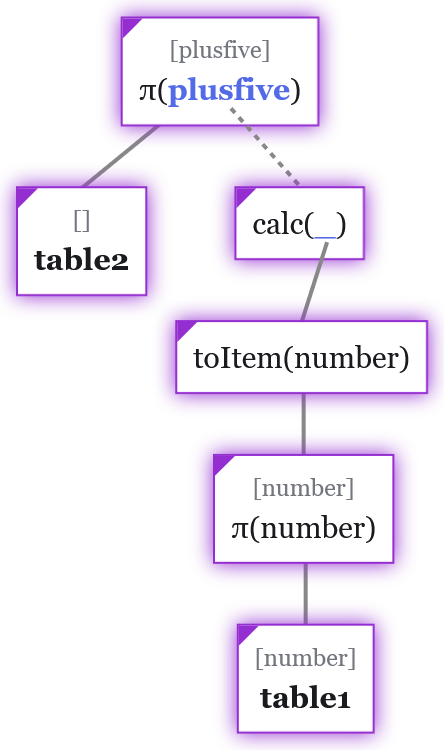
\includegraphics[width=\textwidth]{img/tree-unnest-subqueries-before.png}}
    \end{subfigure}\hfill\begin{subfigure}[c]{268pt}
        \centering
        \frame{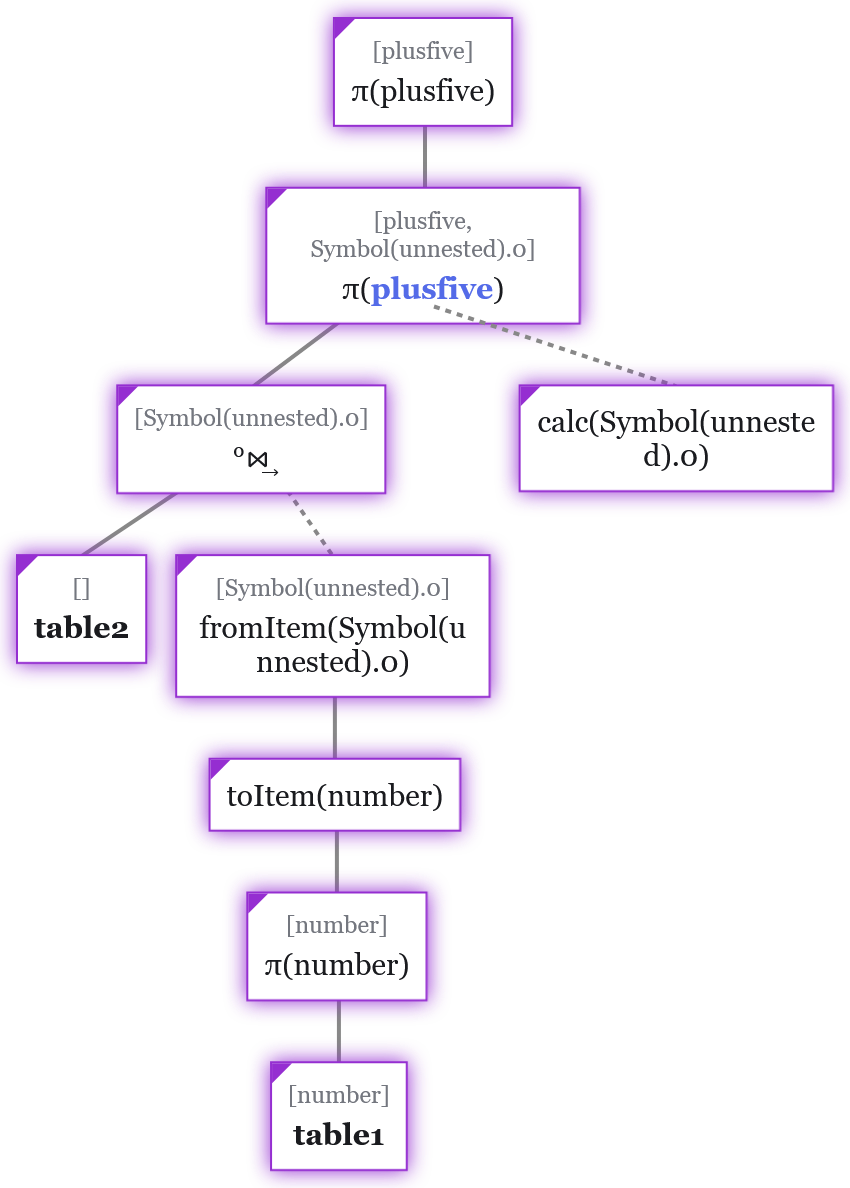
\includegraphics[width=\textwidth]{img/tree-unnest-subqueries-after.png}}
    \end{subfigure}
    
    \caption{An example of an unnested subquery in a \texttt{projection}. The resulting \texttt{projectionConcat} is outer. The redundant \texttt{projection} at the root of the resulting tree is there to ensure the new attribute is stripped away (unnecessary in this case), and will be optimized away by further rules.}
    \label{fig:tree-unnest-subqueries}
\end{figure}

\subsection{Merge to/from items}

As can be seen in figure \ref{fig:tree-unnest-subqueries}, it is possible for \texttt{mapFromItem} to have \texttt{mapToItem} as its source, or vice versa. This happens most often due to query rewriting rules or language switches. The two rules for handling these situations are rather simple -- if \texttt{mapFromItem} is the parent and \texttt{mapToItem} is its source, they become a \texttt{projection} with a single attribute. Otherwise, both operators are simply removed.

\subsection{Pushdown selections}

\texttt{Selections} reduce the cardinality of a tuple stream. It is, therefore, advantageous to process them sooner rather than later. This rule moves \texttt{selections} closer to the leaves of the query tree. The rule considers a continuous sequence of \texttt{selections} and its source operator. The \texttt{selections} which can be pushed below the source are pushed, the rest stay above. The rule is then applied again to the pushed-down \texttt{selections}.

A \texttt{selection} can always be safely pushed below \texttt{orderBy} and \texttt{distinct}. It can also always be pushed down below set operators like \texttt{union} or \texttt{difference}, but it needs to be duplicated and applied to both source branches. \texttt{Selections} can also be swapped with \texttt{projections}, as long as the \texttt{selections} do not rely on any new attributes calculated by the \texttt{projections}. If they depend on renamed attributes, the \texttt{selections} must be modified appropriately. It may not always be possible to rename the \texttt{selection}. When it comes to \texttt{joins} and \texttt{cartesianProducts}, the \texttt{selections} can be pushed into branches that contain all necessary attributes for evaluating the conditions, as long as the \texttt{join} is not left outer and it is not its right branch or vice versa.

\begin{figure}[htpb]
    \begin{subfigure}[b]{\textwidth}
    \begin{tcolorbox}[colback=white, colframe=black, boxrule=1pt, arc=0pt]
        \begin{minted}[fontsize=\small]{sql}
SELECT t1.x, t2.y
FROM t1 JOIN t2
ON t1.id = t2.id AND t1.x > 17
        \end{minted}
    \end{tcolorbox}
    \end{subfigure}

    \medskip

    \begin{subfigure}[c]{214pt}
        \centering
        \frame{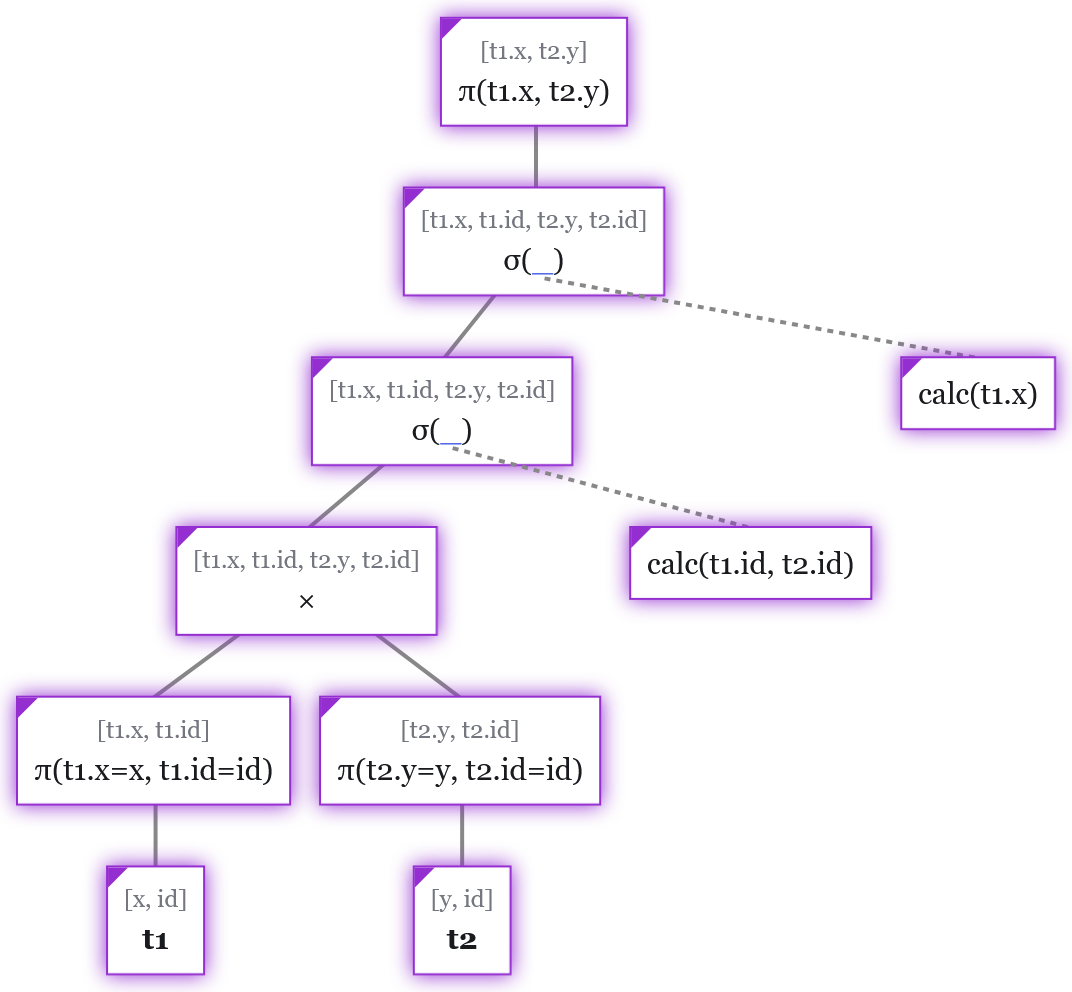
\includegraphics[width=\textwidth]{img/tree-pushdown-selections-before.png}}
    \end{subfigure}\hfill\begin{subfigure}[c]{194pt}
        \centering
        \frame{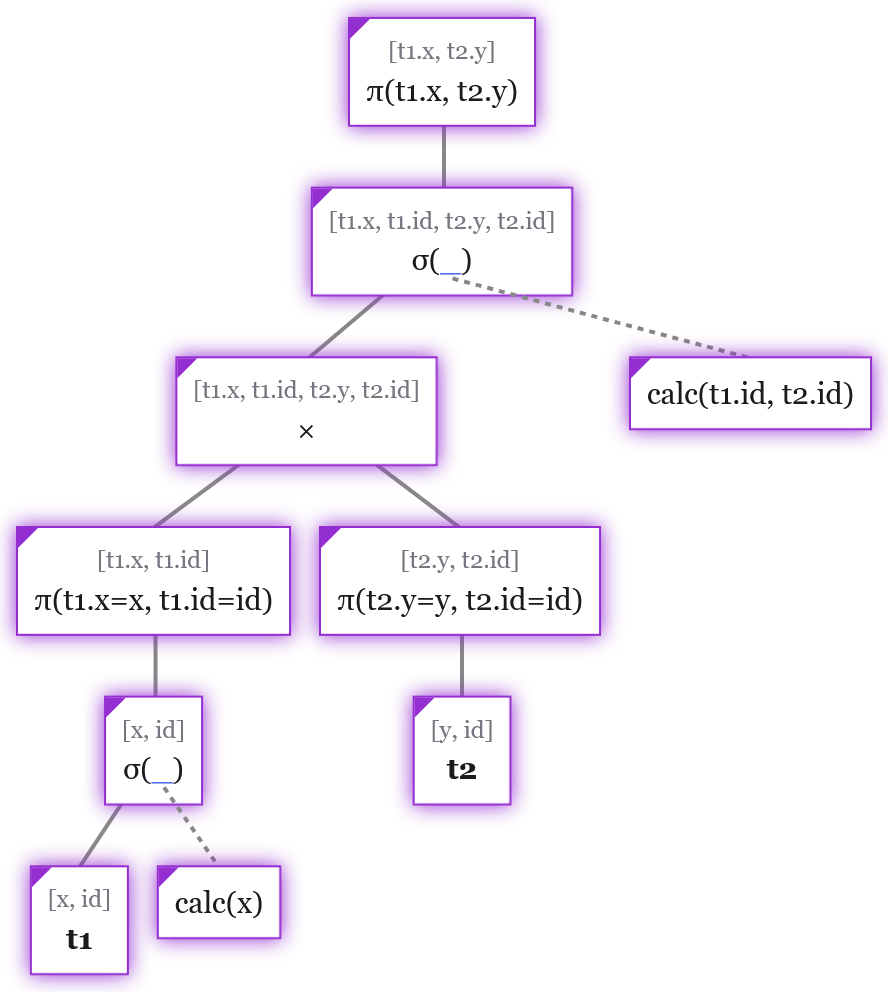
\includegraphics[width=\textwidth]{img/tree-pushdown-selections-after.png}}
    \end{subfigure}
    
    \caption{An example of two \texttt{selections} and a \texttt{cartesianProduct}. The first \texttt{selection} can be pushed into the left branch. The second cannot be pushed anywhere, because it depends on attributes from both branches.}
\end{figure}

\begin{listing}[ht!]
    \begin{minted}[fontsize=\small]{sql}
SELECT t.attr2
FROM (
SELECT t.orig1 AS attr1, t.orig2 AS attr2
FROM t
) AS t
WHERE t.attr1 > (SELECT t.orig1 FROM t2 AS t)
    \end{minted}
    \caption{An overly contrived example where it is not possible to fully push the \texttt{selection} into the \texttt{t2} subquery due to renaming collisions.}
    \label{fig:cannot-rename}
\end{listing}

\subsection{ProjectionConcat to join}

\texttt{ProjectionConcat} may be converted to a \texttt{cartesianProduct} or a left \texttt{join} when its \texttt{mapping} does not depend on the \texttt{source} context (the subquery is not correlated). If the \texttt{projectionConcat} has the \texttt{validateSingleValue} flag set (see section \ref{subsec:unnest-subqueries}), the flag is transferred to the new operator.

\subsection{Products to joins}

This rule merges \texttt{selections} with subsequent \texttt{cartesianProducts} into \texttt{joins}. The resulting \texttt{join} will have multiple conditions instead of a single combined one.

\subsection{Join indices, Index scans}

The two rules responsible for DortDB secondary indices, as described in section \ref{sec:indices}. The first rule detects indexable expressions in \texttt{join} conditions. The \texttt{join} is transformed into a \texttt{projectionConcat} with a \texttt{selection}. The second rule then detects indexable \texttt{selections} and data sources and combines them into \texttt{indexScans}.

\subsection{Merge projections}

This is likely the most complex rule currently implemented in the DortDB optimizer. It combines subsequent \texttt{projections} into a single one when possible. Unused attributes are removed. Calculated attributes are merged as long as the calculation is only referenced once.

\begin{figure}[htpb]
    \begin{subfigure}[b]{\textwidth}
    \begin{tcolorbox}[colback=white, colframe=black, boxrule=1pt, arc=0pt]
        \begin{minted}[fontsize=\small]{sql}
SELECT t.a1, t.a2, t.c1, t.c3 + t.a1 AS c4
FROM (
  SELECT t.a1, t.a2, t.c1, t.c2 * 2 AS c3, t.unused
  FROM (
    SELECT a1, a2, a3 * 2 AS c1, a4 * 2 AS c2, unused
    FROM t
  ) AS t
) AS t
        \end{minted}
    \end{tcolorbox}
    \end{subfigure}

    \medskip

    \begin{subfigure}[c]{234pt}
        \centering
        \frame{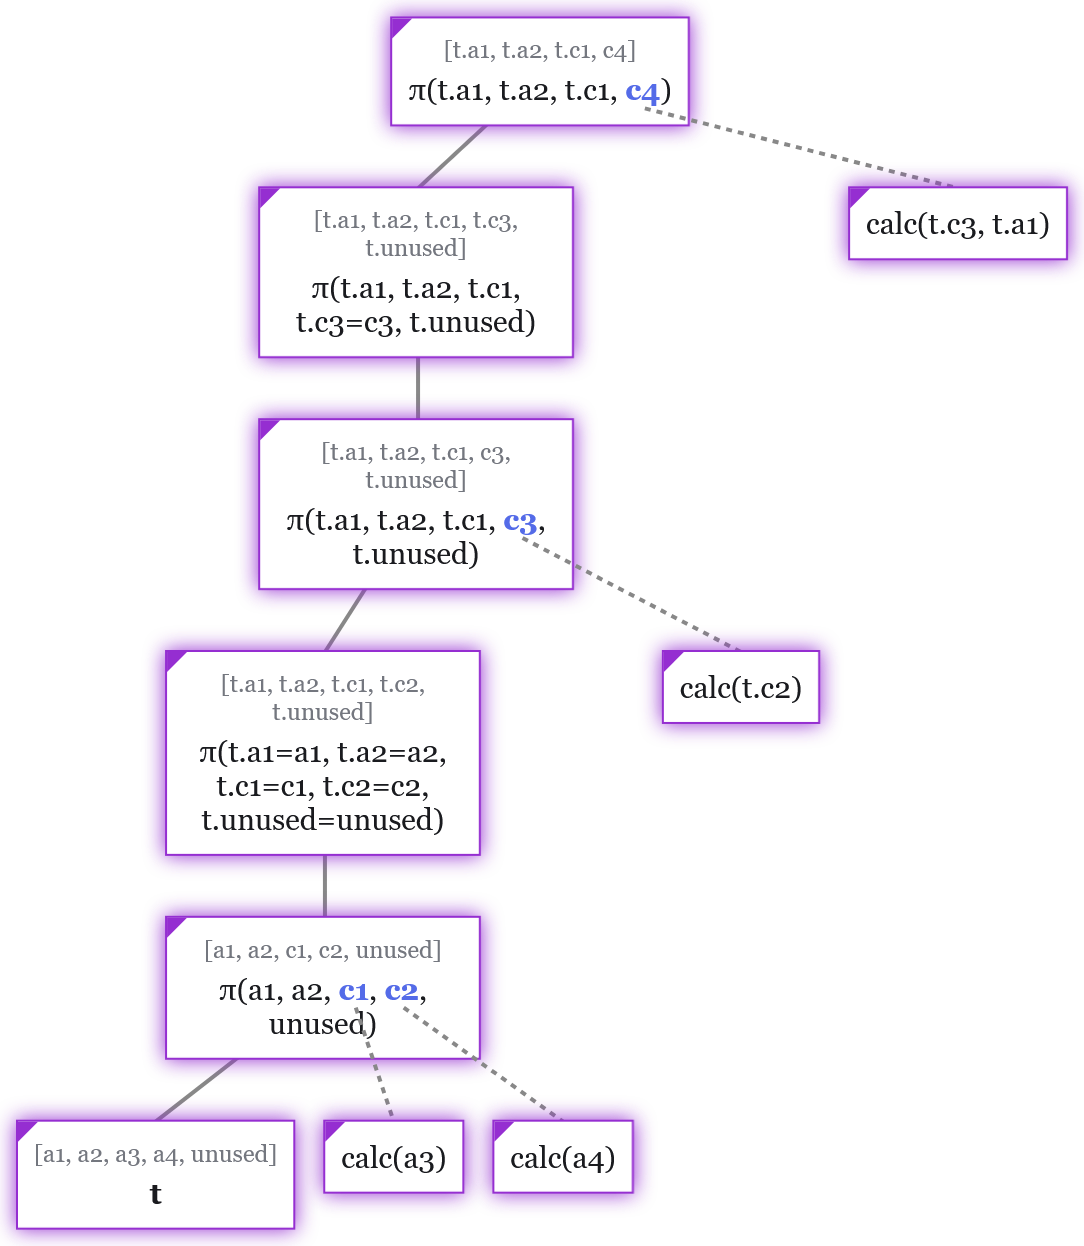
\includegraphics[width=\textwidth]{img/tree-merge-projections-before.png}}
    \end{subfigure}\hfill\begin{subfigure}[c]{174pt}
        \centering
        \frame{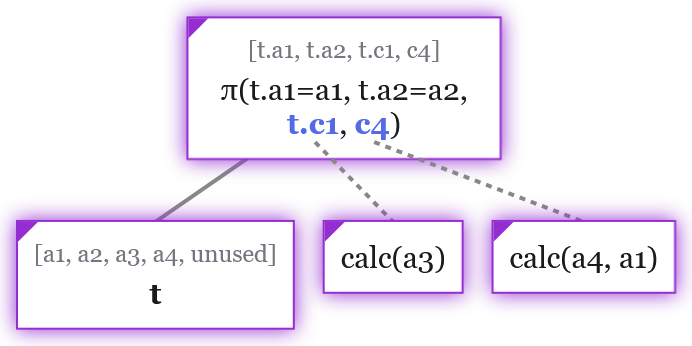
\includegraphics[width=\textwidth]{img/tree-merge-projection-after.png}}
    \end{subfigure}
    
    \caption{An example of multiple merged \texttt{projections}. The \texttt{unused} attribute is removed. Calculated attributes are merged into more complex calculations. If the outer query selected \texttt{t.c1} twice, some merging would be prevented in order to avoid recomputing potentially expensive calculations multiple times. The final query tree would contain two \texttt{projections}.}
\end{figure}

\section{Calculation building}
\label{sec:calc-building}

\texttt{Calculations} are usually created from intermediary plan operators such as \texttt{FnCalls}. This process aims to create a single final callable. \texttt{FnCalls} can be marked as \textit{pure}. If arguments of pure \texttt{FnCalls} are constant (represented by \texttt{literal} plan operators), the function is precomputed and replaced by a \texttt{literal} containing the result. This way, redundant computation may be avoided. During the building process, SQL-style \texttt{quantifiers} combined with specific comparison operators are optimized using rules specified in \cite{holsch2016optimization}.
\chapter{Benchmarks}
\label{chap:benchmarks}

% arango import: 20s
% orientdb import: 424

In the previous chapters, we have introduced the concept of language switching and the unified algebra. We have implemented three query languages and various optimizations. Next, we will evaluate DortDB and see how we fare compared to other established solutions. We will first examine the viability of our approach on multimodel workloads. Then, we will focus on DortDB as a framework for SQL in JavaScript environments.

All of the experiments were conducted on a machine with a 12-core AMD Ryzen 9 7900 CPU, a 32 GB 6000 MHz RAM, and an SSD.

\section{UniBench}
\label{sec:unibench}

UniBench\cite{zhang2018unibench} is a benchmark designed for evaluating multimodel databases. It provides a data model simulating \textit{social commerce}, a combination of social media and E-commerce. We will use a pre-generated 1 GB dataset, as well as a smaller sample created by selecting data about a hundred customers, which is 5 MB in size. Besides data, the benchmark specifies 10 analytical queries combining relational, document, and graph data models. The queries are described in natural language and need to be rewritten for each tested system, as different multimodel databases use different query languages. The queries used by DortDB are included in appendix \ref{apx:unibench-queries}.

\begin{figure}[!ht]
    \centering
    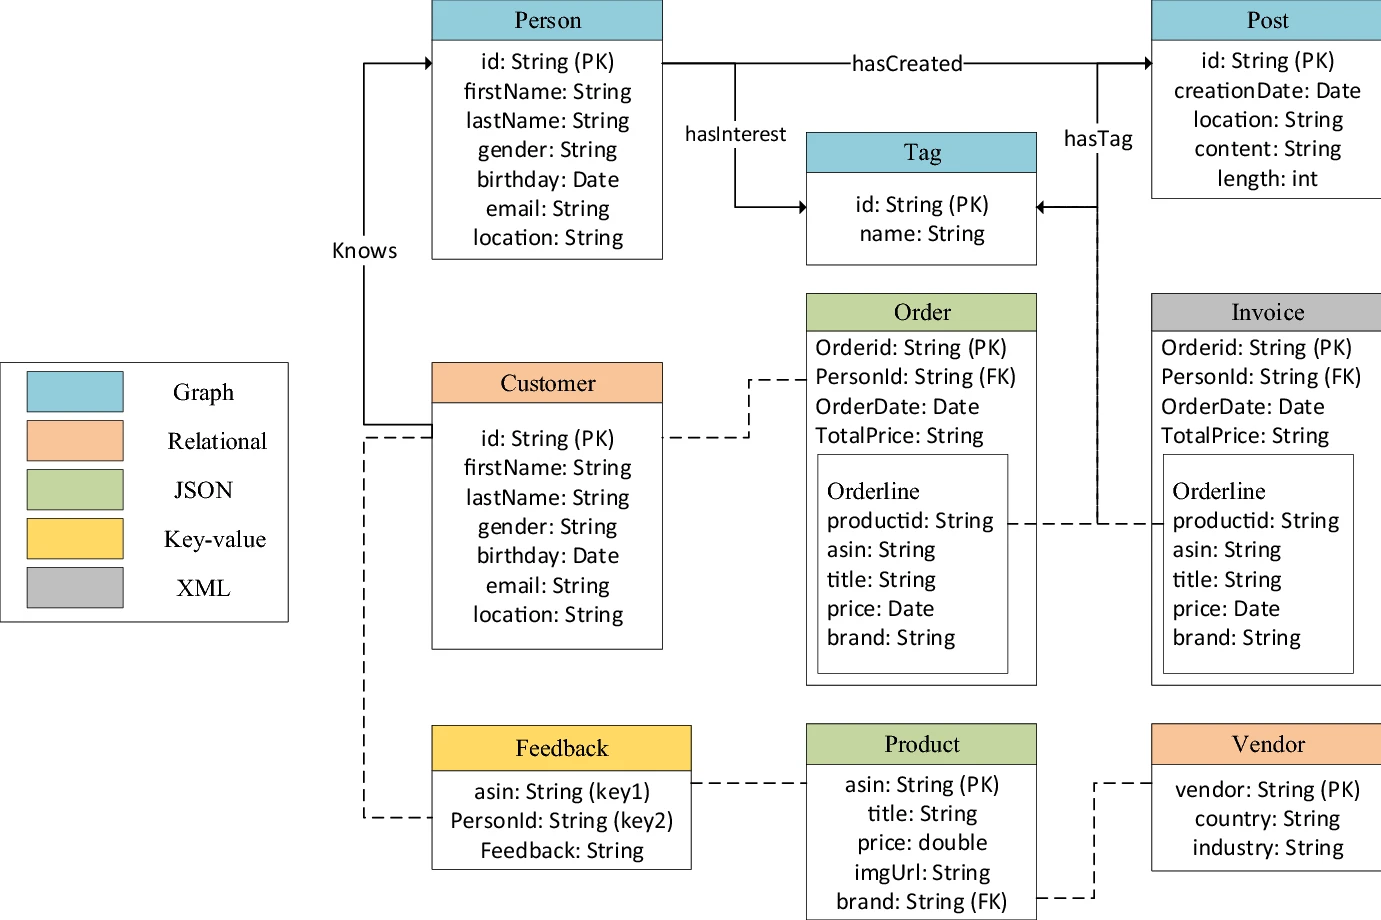
\includegraphics[width=\linewidth]{img/unibench-schema.png}
    \caption{Schema of the UniBench data model\cite{zhang2021holistic}.}
\end{figure}

Part of the UniBench repository are example queries for ArangoDB\footnote{\url{https://arangodb.com/}} and OrientDB\footnote{\url{https://orientdb.dev/}}, as well as scripts for importing data into the database systems. We have used OrientDB version 2.2.16, the same as in the original paper, because the importing mechanisms have changed since, and the provided scripts could not be used otherwise. The importing scripts had to be slightly modified anyway, and we had to configure several indices and vertex properties in the database schema in order for the OrientDB queries to work. The ArangoDB version used was 3.12.5, the latest at the time of writing. There were no issues with either the ArangoDB data import or the ArangoDB queries.

\subsection{Data import}

We have measured the time it takes to import data into the system. In DortDB, the UniBench data was uncompressed from a zip archive, parsed, and stored in memory. Additionally, the data sources were indexed. This was done multiple times and averaged. The ArangoDB and OrientDB measurements come from the provided import scripts, and the data was imported only once.

\begin{listing}[!ht]
\begin{minted}{ts}
db.createIndex(['defaultGraph', 'nodes'], [], ConnectionIndex);
db.createIndex(['defaultGraph', 'nodes'], ['x.id'], MapIndex, {
  mainLang: 'cypher',
  fromItemKey: ['x'],
});
db.createIndex(['defaultGraph', 'edges'], [], ConnectionIndex);
db.createIndex(['customers'], ['id'], MapIndex);
db.createIndex(['products'], ['productId'], MapIndex);
db.createIndex(['products'], ['brand'], MapIndex);
db.createIndex(['products'], ['asin'], MapIndex);
db.createIndex(['feedback'], ['productAsin'], MapIndex);
db.createIndex(['brandProducts'], ['brandName'], MapIndex);
db.createIndex(['brandProducts'], ['productAsin'], MapIndex);
db.createIndex(['vendors'], ['id'], MapIndex);
db.createIndex(['posts'], ['id'], MapIndex);
db.createIndex(['orders'], ['PersonId'], MapIndex);
\end{minted}
\caption{Indices created on DortDB UniBench data sources.}
\end{listing}

\begin{figure}[!ht]
    \centering
    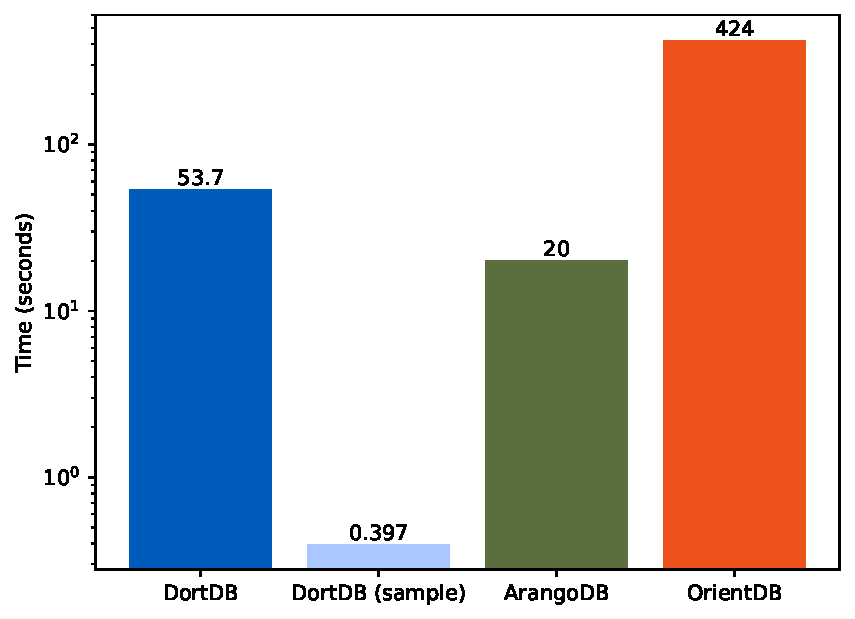
\includegraphics[width=0.6\linewidth]{img/unibench-init.pdf}
    \caption{Processing time for data import.}
    \label{fig:unibench-init}
\end{figure}

The results are displayed in Figure \ref{fig:unibench-init}. Disregarding the sampled dataset, ArangoDB was more than twice as fast as DortDB, even though DortDB did not write anything to disk. One possible explanation is that DortDB runs in a single thread, while ArangoDB is multithreaded. OrientDB data import took around 7 minutes, which is within the realm of expectation.

\subsection{Query performance}

Each query was executed multiple times, and the execution times were averaged. Most of the queries were repeated 10 times, except for DortDB queries that took more than 3 hours or failed. Some of the queries are designed as parametrized, for example, a query that fetches all information available on a certain customer. These parameters were randomized for each execution and taken from a pool provided as part of the dataset.

\begin{figure}[!ht]
    \centering
    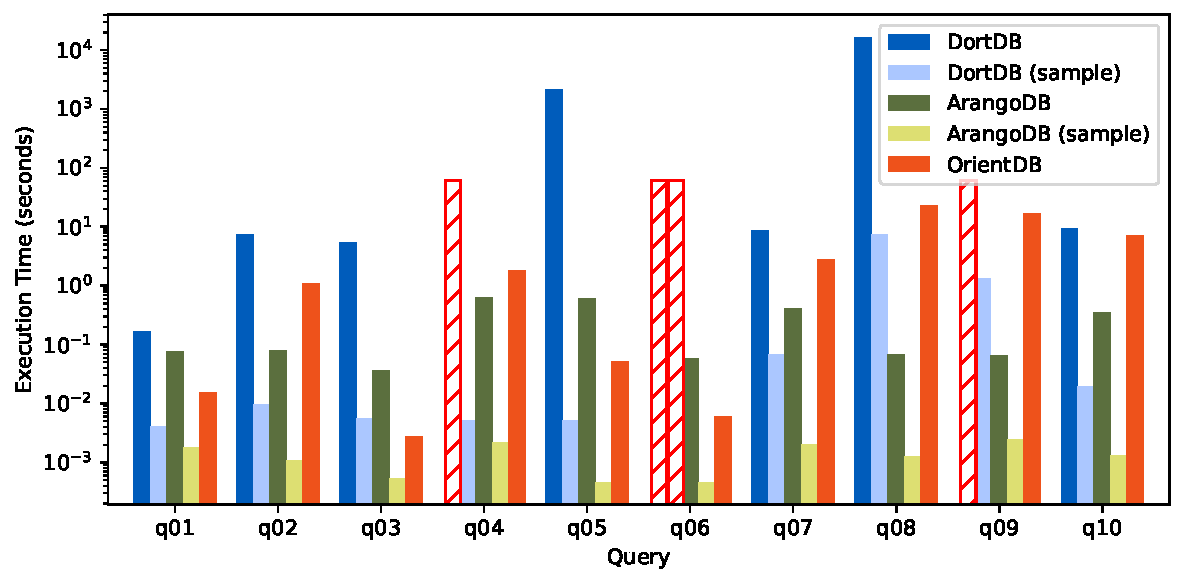
\includegraphics[width=\linewidth]{img/unibench-execution.pdf}
    \caption{Average execution time for each query.}
    \label{fig:unibench-execution}
\end{figure}

The results can be seen in Figure \ref{fig:unibench-execution}. Interestingly enough, OrientDB outperforms ArangoDB in several queries, which contrasts with the measurements in the original paper. On the other hand, DortDB is the slowest, in some cases, more than a hundred times. Three of the DortDB queries failed due to running out of memory. In queries 4 and 6, this is caused by recursive graph traversal. Query 6 ran out of memory even on the small data sample, because its goal was to find the shortest path between two customers, and the randomized customers from the sample were not connected at all. Query 9 does not feature any recursion, and the reasons for its high memory consumption are less immediately recognizable. The query features a large number of logical operators that materialize the whole underlying data stream, such as \texttt{orderBy} or \texttt{treeJoin}. Other databases may avoid this problem by saving intermediary data to disk and using algorithms such as external sorting.

In general, large execution times in DortDB correspond to complex graph traversal and, more markedly, XML tree traversal. The framework currently does not feature any XML tree access optimizations besides the general optimizer rules, nor does it feature any XML indices.

In query 8, the XQuery subquery passes tuple data to SQL as an XML element. We have tested an alternate version of the query without the XML element, and the performance difference was negligible.

On the other hand, DortDB works well with relational data and aggregating queries such as query 10. While it never outperforms any of the competing database systems, we need to remember that it runs in an interpreted language and in a single thread.

\subsection{Query memory usage}

The previous section highlighted a vital problem for in-memory databases: memory consumption. The statistics for DortDB were collected by invoking the garbage collector immediately before the query and comparing the process's memory usage before the query starts and after it finishes. This is by no means a completely accurate reflection of the actual query demands, but it gives us some insight. The garbage collector may be invoked during query if necessary, but as long as there is enough available memory, it will simply continue to be filled. We have observed a query fill the entire memory, and the garbage collector freeing 10 GB of space immediately afterwards.

ArangoDB provides peak memory usage as part of its query statistics. OrientDB does not offer such information and does not participate in the results, which are available in Figure \ref{fig:unibench-memory}.

\begin{figure}[!ht]
    \centering
    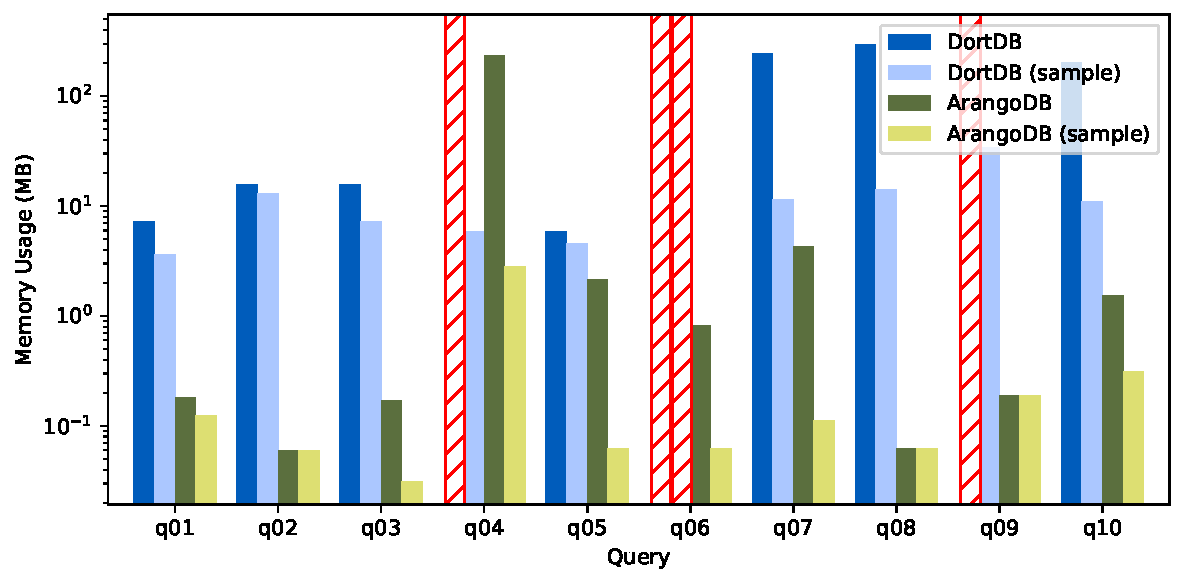
\includegraphics[width=\linewidth]{img/unibench-memory.pdf}
    \caption{Memory usage during each query.}
    \label{fig:unibench-memory}
\end{figure}

We can see that the queries with more materialized operators feature a larger memory usage disparity between DortDB and DortDB (sample). Nevertheless, the difference is never as significant as the difference between dataset sizes. A notable curiosity is query 4, where the sample DortDB memory usage is smaller than in query 3, while on the full dataset, the DortDB ran out of memory. This is because the query iterates over all three-hop common friends of two customers, which are actually not connected in the sample data, and there is therefore nothing to iterate over.

\section{SQL}
\label{sec:sql-benchmarks}

Many benchmarks are available for SQL databases, but the TPC-H\footnote{\url{https://www.tpc.org/tpch/}} is perhaps the best known. It features 22 analytical queries with a moderate to high level of complexity. We have generated data and the queries with an open-source alternative to the official benchmark\footnote{\url{https://github.com/gregrahn/tpch-kit}}. The data was generated with a scale factor of 0.1, resulting in 100 MB of data. The queries were slightly modified for each database in order to adapt to different flavors of SQL. Query 15 was skipped altogether, because it features a \texttt{CREATE VIEW} clause and DortDB does not support either that or \texttt{WITH} common table expressions. The queries are available in appendix \ref{apx:tpch-queries}.

\begin{figure}
    \centering
    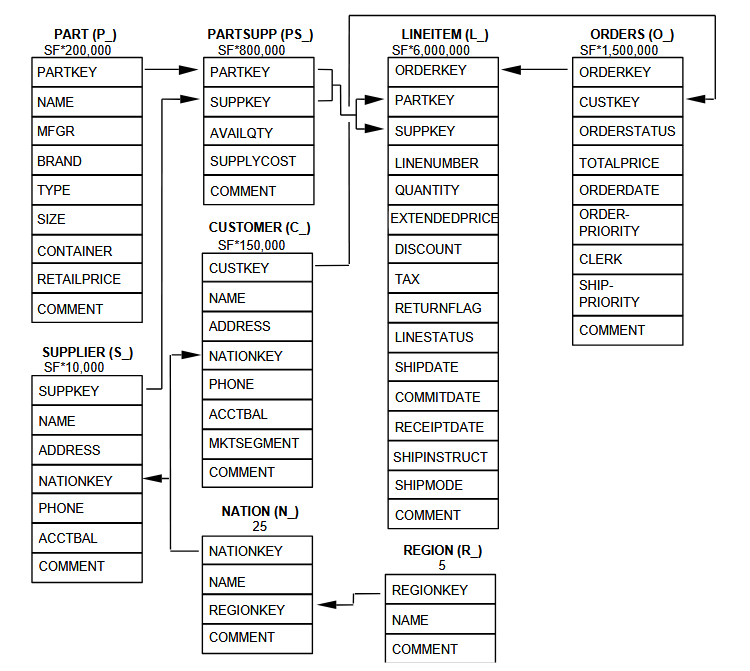
\includegraphics[width=0.7\linewidth]{img/tpch-schema.png}
    \caption{TPC-H benchmark schema. Taken from the TPC-H specification\protect\footnotemark.}
\end{figure}

\footnotetext{\url{https://www.tpc.org/TPC_Documents_Current_Versions/pdf/TPC-H_v3.0.1.pdf}}

\begin{listing}[!ht]
\begin{minted}{ts}
db.createIndex(['customer'], ['custkey'], MapIndex);
db.createIndex(['customer'], ['nationkey'], MapIndex);
db.createIndex(['lineitem'], ['orderkey'], MapIndex);
db.createIndex(['lineitem'], ['partkey'], MapIndex);
db.createIndex(['lineitem'], ['suppkey'], MapIndex);
db.createIndex(['nation'], ['nationkey'], MapIndex);
db.createIndex(['nation'], ['regionkey'], MapIndex);
db.createIndex(['orders'], ['custkey'], MapIndex);
db.createIndex(['orders'], ['orderkey'], MapIndex);
db.createIndex(['part'], ['partkey'], MapIndex);
db.createIndex(['partsupp'], ['partkey'], MapIndex);
db.createIndex(['partsupp'], ['suppkey'], MapIndex);
db.createIndex(['region'], ['regionkey'], MapIndex);
db.createIndex(['supplier'], ['suppkey'], MapIndex);
db.createIndex(['supplier'], ['nationkey'], MapIndex);
\end{minted}
\caption{Indices created for the TPC-H benchmark.}
\end{listing}

We have compared DortDB with two other JavaScript in-memory SQL data\-bases. SQL.js\footnote{\url{https://sql.js.org/}} is SQLite\footnote{\url{https://sqlite.org/}} compiled into WebAssembly, while AlaSQL\footnote{\url{https://github.com/AlaSQL/alasql}} is a rich implementation of SQL with many features. Each query was run up to 10 times, but no longer than an hour. The averaged results are in Figure \ref{fig:tpch-execution}.

\begin{figure}[!ht]
    \centering
    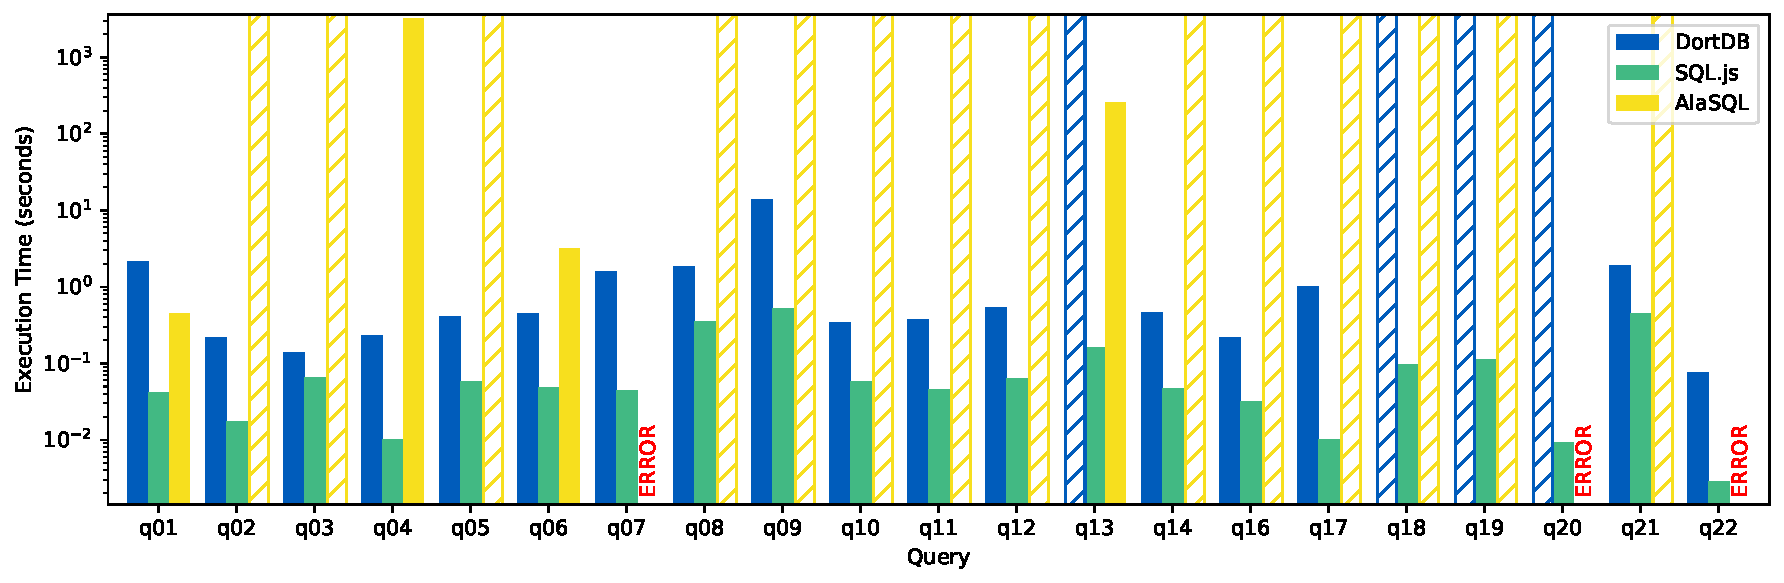
\includegraphics[width=\linewidth]{img/tpch-execution.pdf}
    \caption{Average execution time for each query.}
    \label{fig:tpch-execution}
\end{figure}

It comes as no surprise that SQL.js achieved the best execution times. It runs in native code, and its query optimizer is very powerful, owing to more than 20 years of development. Compared to that, AlaSQL timed out most of the queries and crashed on three. According to its GitHub wiki, it does not have a query optimizer per se, but it preemptively indexes tables before joining, and it tries to push down \texttt{WHERE} conditions before joins. This, unfortunately, does not fare that well when faced with more complex queries. When the queries are simple, like query 1, which focuses on aggregating multiple columns at once, AlaSQL can outperform DortDB thanks to its precompiled queries. Instead of executing a plan in the form of a tree, AlaSQL compiles it into a single function as a concatenation of source code.

DortDB managed most of the queries quite well, timing out on four. Query 13 contains a \texttt{LIKE} comparison with three \texttt{\%} wildcards. Queries 18 and 20 contain complex \texttt{IN} operators, which are currently not optimized. Finally, query 19 tests the optimization of \texttt{OR} conditions, which is also not implemented.
\chapter{Implementation}
\label{chap:implementation}

DortDB is a collection of TypeScript libraries. Its source code is available as an appendix to this thesis, as well as online at \href{https://github.com/filipjezek/dortdb}{https://github.com/filipjezek/dortdb}. All the libraries are part of a single monorepository managed with Nx\footnote{\url{https://nx.dev/}}. The \texttt{@dortdb/core} is the main library containing the core of the framework. There is a separate library for each of the currently implemented languages (\texttt{@dortb/lang-cypher}, \texttt{@dortdb/lang-sql}, and \texttt{@dortdb/lang-xquery}). Additionally, there are packages for the GUI and benchmarks (\texttt{@dortdb/showcase} and \texttt{@dortdb/benchmarks}). Finally, \texttt{@dortdb/dataloaders} contains utilities for importing data from various formats.

\begin{figure}[htpb]
    \centering
    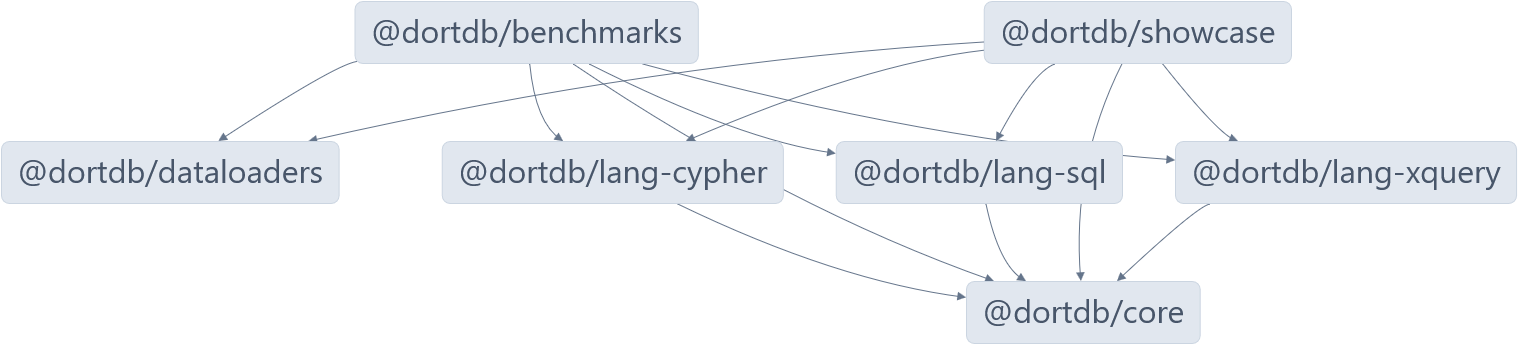
\includegraphics[width=\textwidth]{img/packages-graph.png}
    \caption{Dependency graph of the monorepository.}
\end{figure}

\section{Core library}

The core library serves as a common framework for registering data sources, querying, and optimization. The individual languages are responsible for converting a text query into a logical plan. The plan operator tree implements an extended version of the visitor design pattern\cite{johnson1995design}. In order for each language to be able to expand the plan algebra with its own operators, or to customize the behavior defined for a common operator, the design pattern is modified to take into account the language that instantiates each plan operator, as seen in Figure \ref{fig:visitor-pattern}. The \texttt{accept} method accepts a dictionary of visitors instead of a single visitor. The core library provides a default implementation of a visitor for each phase of the query process. The individual languages may specify their own implementations, usually by extending the original class. The \texttt{accept} and \texttt{visit} methods also optionally take a second argument, which may be necessary to propagate information during the downward pass of the plan tree, for example, the existing context during plan execution.

\begin{listing}[ht!]
    \begin{minted}[fontsize=\small]{ts}
export interface PlanOperator {
  lang: Lowercase<string>;

  accept<Ret, Arg>(
    visitors: Record<string, PlanVisitor<Ret, Arg>>,
    arg?: Arg,
  ): Ret;

  // ...
}
    
export interface PlanVisitor<Ret, Arg = never> {
  visitRecursion(operator: Recursion, arg?: Arg): Ret;
  visitItemSource(operator: ItemSource, arg?: Arg): Ret;
  visitProjection(operator: Projection, arg?: Arg): Ret;
  // ...
}

export class ItemSource implements PlanOperator {
  constructor(
    public lang: Lowercase<string>,
    public name: ASTIdentifier | Aliased<ASTIdentifier>,
  ) {}

  accept<Ret, Arg>(
    visitors: Record<string, PlanVisitor<Ret, Arg>>,
    arg?: Arg,
  ): Ret {
    return visitors[this.lang].visitItemSource(this, arg);
  }

  // ...
}
    \end{minted}
    \caption{The extended visitor pattern used in the logical plan.}
    \label{fig:visitor-pattern}
\end{listing}

\subsection{Language manager}

Each language can define its own visitors, callables, or aggregates. Callables and aggregates may also be provided as an extension, not scoped to any specific language. For example, a datetime extension might define operators and functions for manipulating datetime values. The \texttt{LanguageManager} class then handles instantiating of visitor dictionaries or finding an aggregate or callable by name.

\section{Query process}

The rest of the library's key components will be outlined in the order they appear during query execution. Different languages may handle some steps differently. The key deviations will be noted when appropriate.

\subsection{Lexer and parser}

First of all, the text query needs to be parsed into an \textit{abstract syntax tree (AST)}. In order to do this, \textit{parser generators} are used. Modern projects use solutions such as \texttt{ANTLR}\footnote{\url{https://www.antlr-ng.org/}}. We have used 
\texttt{ts-jison}\footnote{\url{https://github.com/ericprud/ts-jison}} instead, which is based on \texttt{GNU Bison}\footnote{\url{https://www.gnu.org/software/bison/}}. \texttt{Bison} employs an older approach less compatible with modern software engineering practices. The resulting parser and its runtime are, however, significantly smaller (approximately 10 times).

The parser is generated from a formal grammar file. \texttt{ts-jison} in fact generates two components. The \textit{lexer} handles the lexical analysis, converting the text query into tokens such as a specific keyword or a string. The parser then combines the tokens into grammar constructs like a function call or a \texttt{SELECT} statement. The resulting AST nodes implement the visitor pattern, similarly to the logical plan.

\subsection{Plan builder}

The AST is converted into a logical plan using a \texttt{PlanBuilder} visitor. It is possible to apply some optimizations while creating the plan, but the resulting plan is mostly a literal representation of the original query. Intermediary operators are converted into \texttt{calculations} right at this stage, in a process more closely described in section \ref{sec:calc-building}. The SQL language creates the plan in two passes, for reasons detailed in section \ref{subsec:sql-schema-data-sources}. The plan builder is provided the current context in order to determine which attributes are variables or columns, etc, and which should be considered data sources. Some languages (like SQL) do not know the full context when building plans for nested language subqueries. The context, therefore, also includes information on data sources whose schema is being inferred. The plan builder should, in addition to the plan, create a set of newly identified identifiers. See Program \ref{fig:plan-builder-outer-ctx} for an example.

\begin{listing}[!ht]
\begin{minted}{sql}
SELECT attr1 FROM t1
WHERE EXISTS (
  LANG xquery
\end{minted}
\nestedMintedVspace
\begin{minted}[style=manni]{xquery}
  $Invoices//[OrderId = $t1:attr2]
\end{minted}
\nestedMintedVspace
\begin{minted}{sql}
)
\end{minted}
\caption{The plan builder for XQuery receives context with \texttt{t1.attr1} and with \texttt{t1} set as a data source with not yet identified schema. It then correctly interprets \texttt{\$t1:attr2} as a variable and \texttt{\$Invoices} as a data source. The SQL plan builder then receives back information on \texttt{t1.attr2}.}
\label{fig:plan-builder-outer-ctx}
\end{listing}

\subsection{Optimizer et al.}

The optimizer itself and its rules have their own section elsewhere, see \ref{sec:optimizer}. They make use of multiple other plan visitors.

\begin{description}
    \item[\texttt{EqualityChecker}] A deep equality checker. It is possible to check equality of plan operator trees regardless of their language, or with specific renamings applied. This is helpful, for example, when checking possibly indexable expressions in a \texttt{join} operator, whose input \texttt{tupleSources} are renamed with a \texttt{projection}.
    \item[\texttt{AttributeRenamer}] This visitor renames attributes in an operator tree. Necessary when, e.g., pushing down \texttt{selections} below \texttt{projections}.
    \item[\texttt{AttributeRenameChecker}] It is not always possible to rename attributes without changing the meaning of a query. This visitor verifies that a specific renaming can be done. See figure \ref{fig:cannot-rename} for an example.
    \item[\texttt{TransitiveDependencies}] This visitor extracts dependencies of an operator tree, helping to identify correlated subqueries. As an example, \mint{sql}/SELECT foo.x FROM foo WHERE bar.y > foo.z/ depends on external attribute \texttt{bar.y}. Used in many rules, among others, in selection pushdown or projection merging.
\end{description}

\subsection{Variable mapper}

Attributes used in queries and their plans can generally have multiple components, for example \mintinline{text}{schema.table.column} or \mintinline{xquery}{$qualified:variable}. During query planning and optimization, the attributes are represented as lists of tokens. Sets or maps of attributes are then represented using tries made of nested hash tables. This is fine during planning, but if that were the case during execution and tuples were represented using the same tries, attribute lookups would become prohibitively expensive. In order to optimize this, the \texttt{VariableMapper} visitor renames all attributes as a single number. During execution, tuples are then represented using simple arrays. The numeric attributes are reused when possible to keep the array sizes minimal.

\subsection{Data adapters}

Different data models and different languages may make different assumptions about how the data is stored or represented. In order to decouple logical plans from the data, languages can be configured with data adapters. Data adapters specify how data sources should be accessed. For example, the default XQuery data adapter allows \texttt{treeStep} operators to traverse XML elements. It may, however, be desirable to use XQuery to query JSON data instead. Cypher queries target graphs, which can also be stored in multiple ways. Nodes might be JavaScript objects, and edges might be their properties. The graph might also be stored as a collection of relations, one for each node or edge type. The default Cypher data adapter uses Graphology\cite{guillaume_plique_2025_14835805} as the data backend. The SQL data adapter can be used to override how SQL accesses attributes in relations.

\begin{listing}[ht!]
    \begin{minted}[fontsize=\small]{ts}
export interface XQueryDataAdapter<NodeType = any> {
  isNode(node: unknown): node is NodeType;
  treeStep(test: ASTItemType, axis: AxisType): (node: NodeType) => NodeType[];
  createElement(ns: string, qname: string, content: unknown[]): NodeType;
  createAttribute(ns: string, qname: string, content: string): NodeType;
  createComment(content: string): NodeType;
  createDocument(ns: string, qname: string, content: unknown[]): NodeType;
  createNS(name: string, content: string): NodeType;
  createText(content: string): NodeType;
  createProcInstr(name: string, content: string): NodeType;
  addAttribute(el: NodeType, attr: NodeType): void;
  lookupPrefix(el: NodeType, ns: string): string;
  lookupNSUri(el: NodeType, prefix: string): string;
  atomize(value: unknown): unknown;
}
    \end{minted}
    \caption{The XQuery data adapter interface}
\end{listing}

\subsection{Executor}

Finally, the logical plan is executed. Unlike other visitors, the \texttt{Executor} provided by the core library is abstract and not immediately usable. As was touched upon in previous sections, tuple representations during execution will be different from the actual tuples available in the source data. Each language should therefore extend the \texttt{Executor} and provide its own implementation of the \texttt{visitTupleSource} method.

The default executor implementation makes heavy use of iterators. This comes with a performance impact for smaller datasets, but for larger amounts of data, the difference becomes negligible. This is compensated by memory efficiency. Unless an operator needs to load all of its inputs fully into memory (for example, if it is \texttt{orderBy} or \texttt{groupBy}), the operator produces values on demand lazily. The default executor implementation is fully synchronous and does not support user-defined functions that return promises (e.g., a \texttt{tupleFnSource} which would load a remote JSON document). The visitor pattern, however, makes it easy to make another executor implementation that would add such functionality.

After the query results are produced, tuple values must be serialized into a suitable representation. To this end, each language may specify a serializer function. The default serializer function joins attribute parts with periods and creates a JavaScript object for each tuple.
\chapter{Usage}
\label{chap:usage}

In the previous chapters, we have delved into the design decisions behind DortDB, its implementation, and its theoretical background. However, we have not yet described how to actually use it or extend it. This chapter will serve as a walkthrough through user interaction and as a concise manual for developers. It does not aim to be a full-fledged documentation of DortDB.

\section{Showcase}

DortDB Showcase is a GUI intended as a demonstration of DortDB's capabilities. While it is possible to run the demo locally, the recommended way is to use an instance deployed to GitHub Pages at \url{https://filipjezek.github.io/dortdb}. The Showcase is a purely frontend single page application written in Angular. The user can write queries and inspect their logical plans, experimenting with various optimizer rules. It is also possible to execute the queries on the UniBench sample dataset used in benchmarks in section \ref{sec:unibench}. The rest of this section will consist of a sequence of figures describing various parts of the user interface.

\begin{figure}[!h]
    \centering
    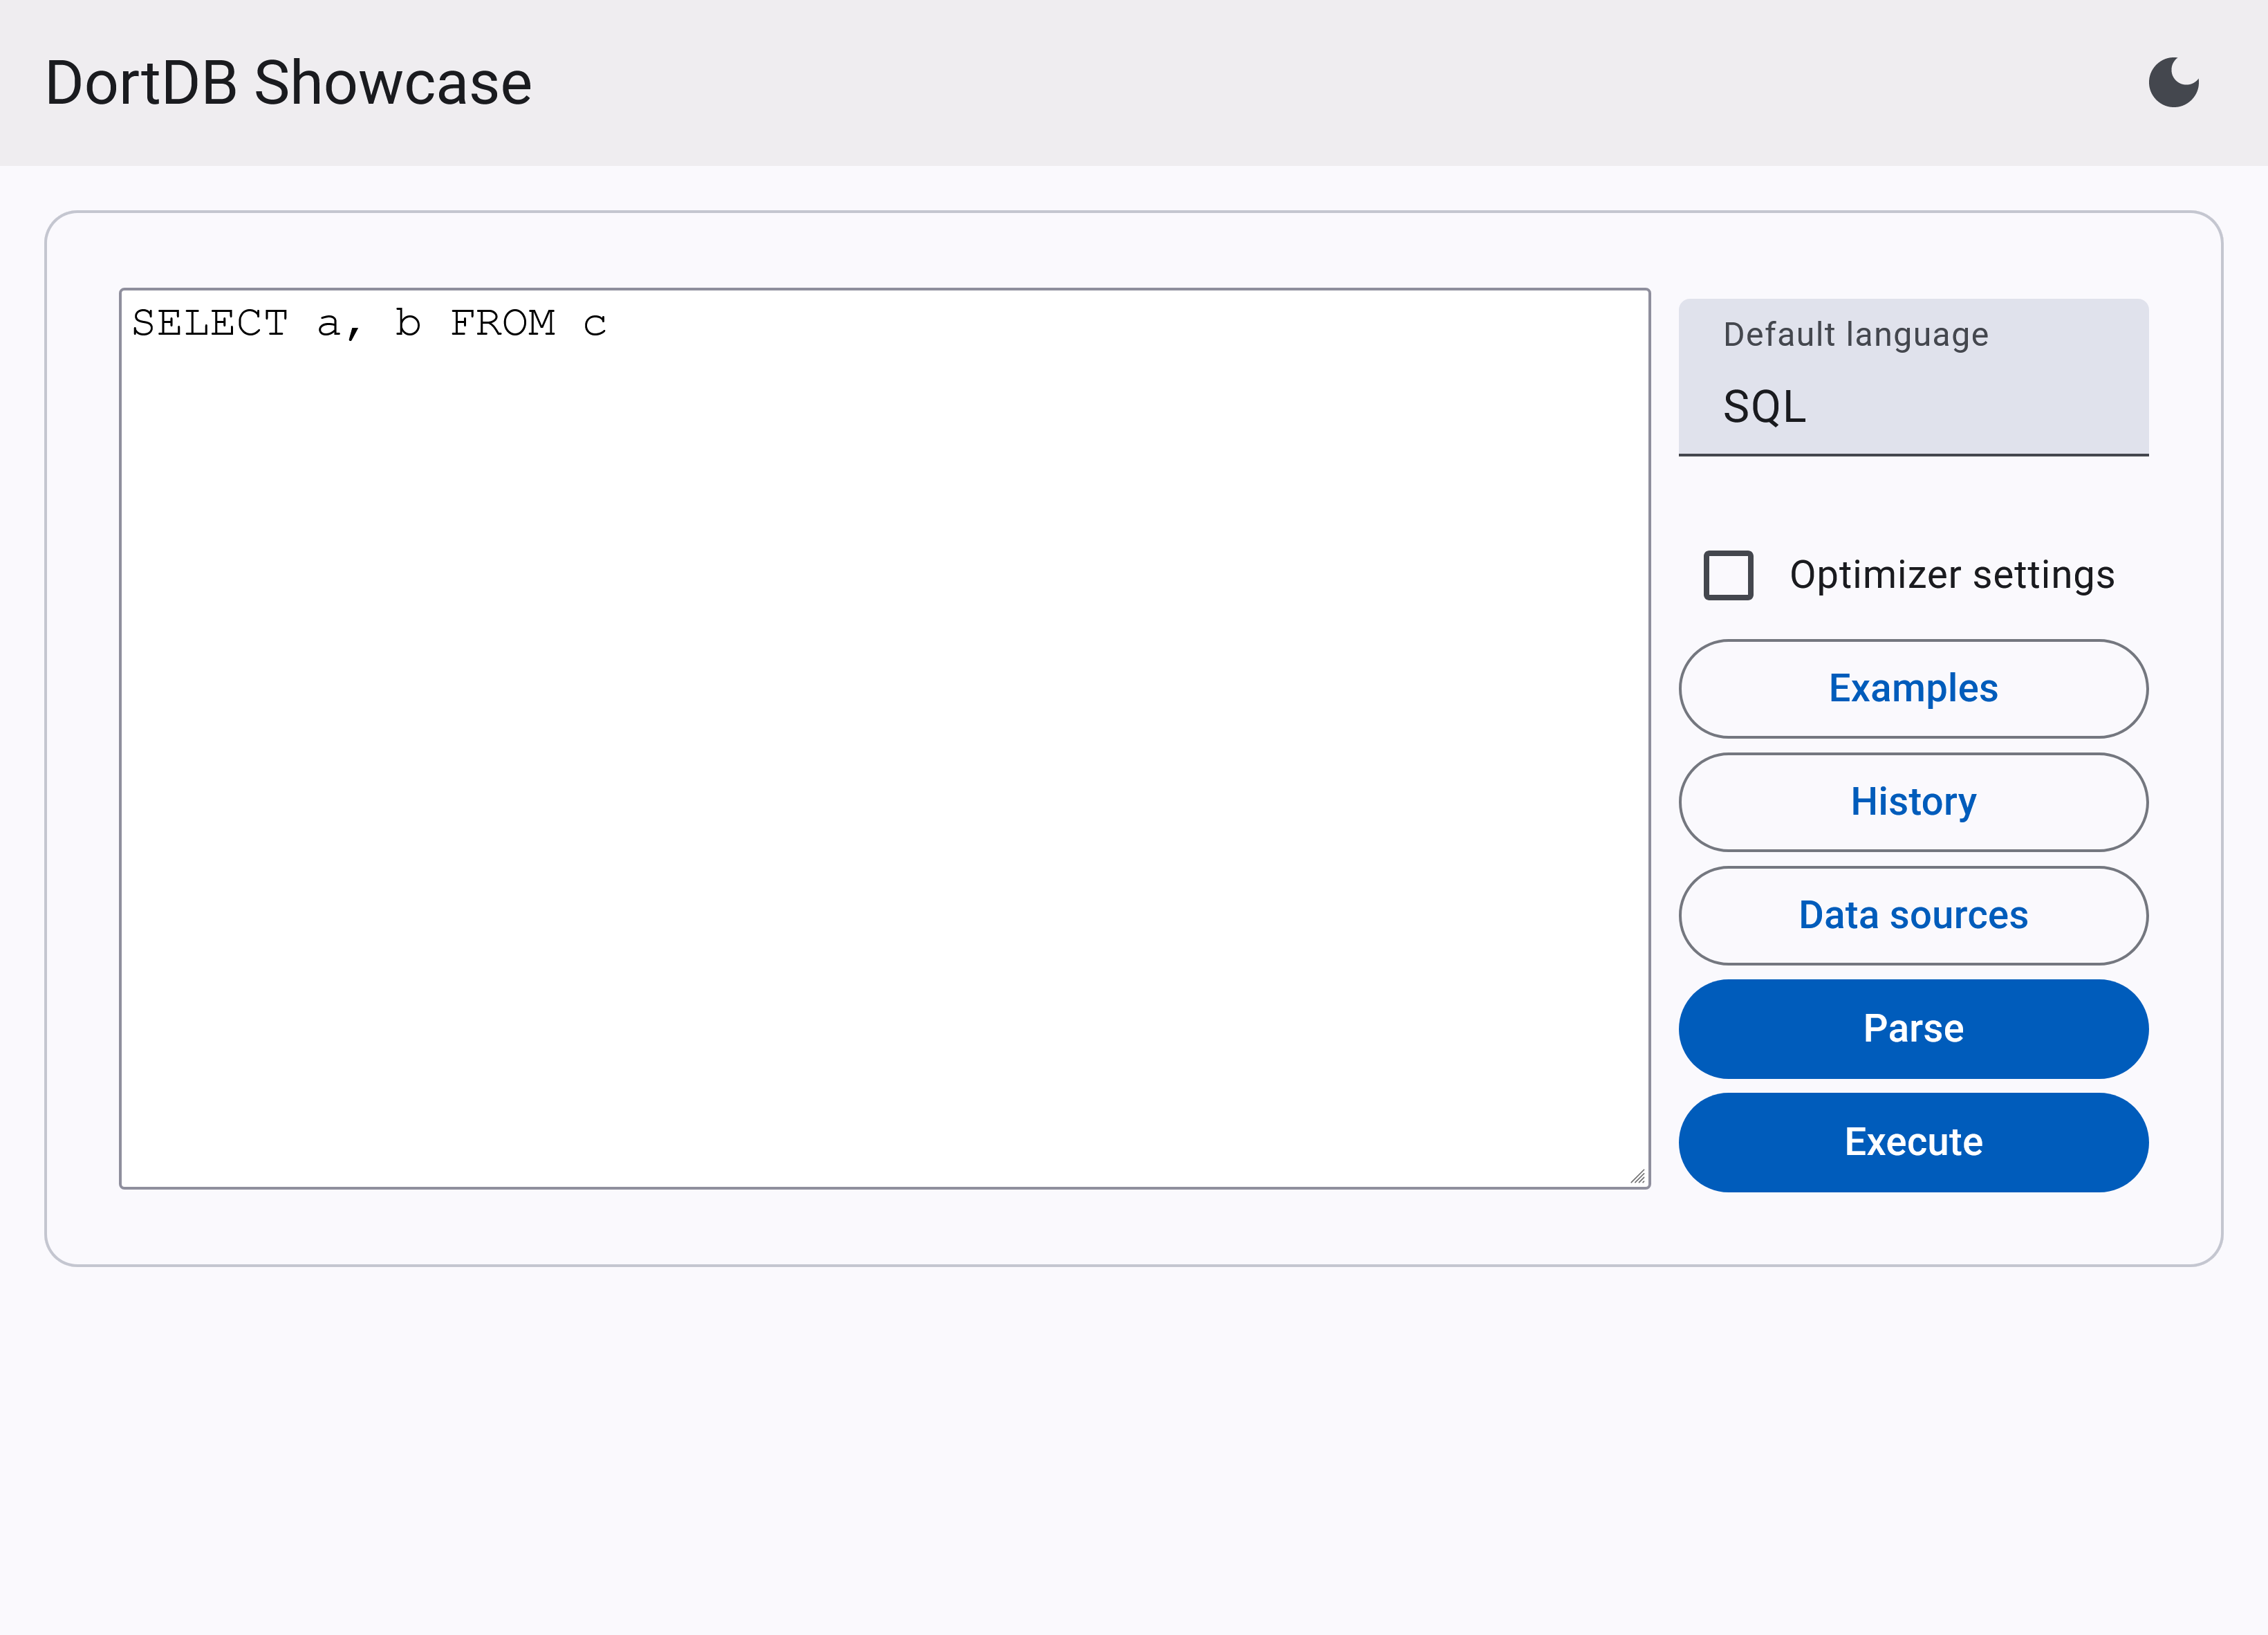
\includegraphics[width=0.8\linewidth]{img/showcase_initial.png}
    \caption{Showcase when loaded in the web browser. The application remembers all settings, including the current query, the optimizer settings, the default language, and query history.}
\end{figure}

\begin{figure}[!h]
    \centering
    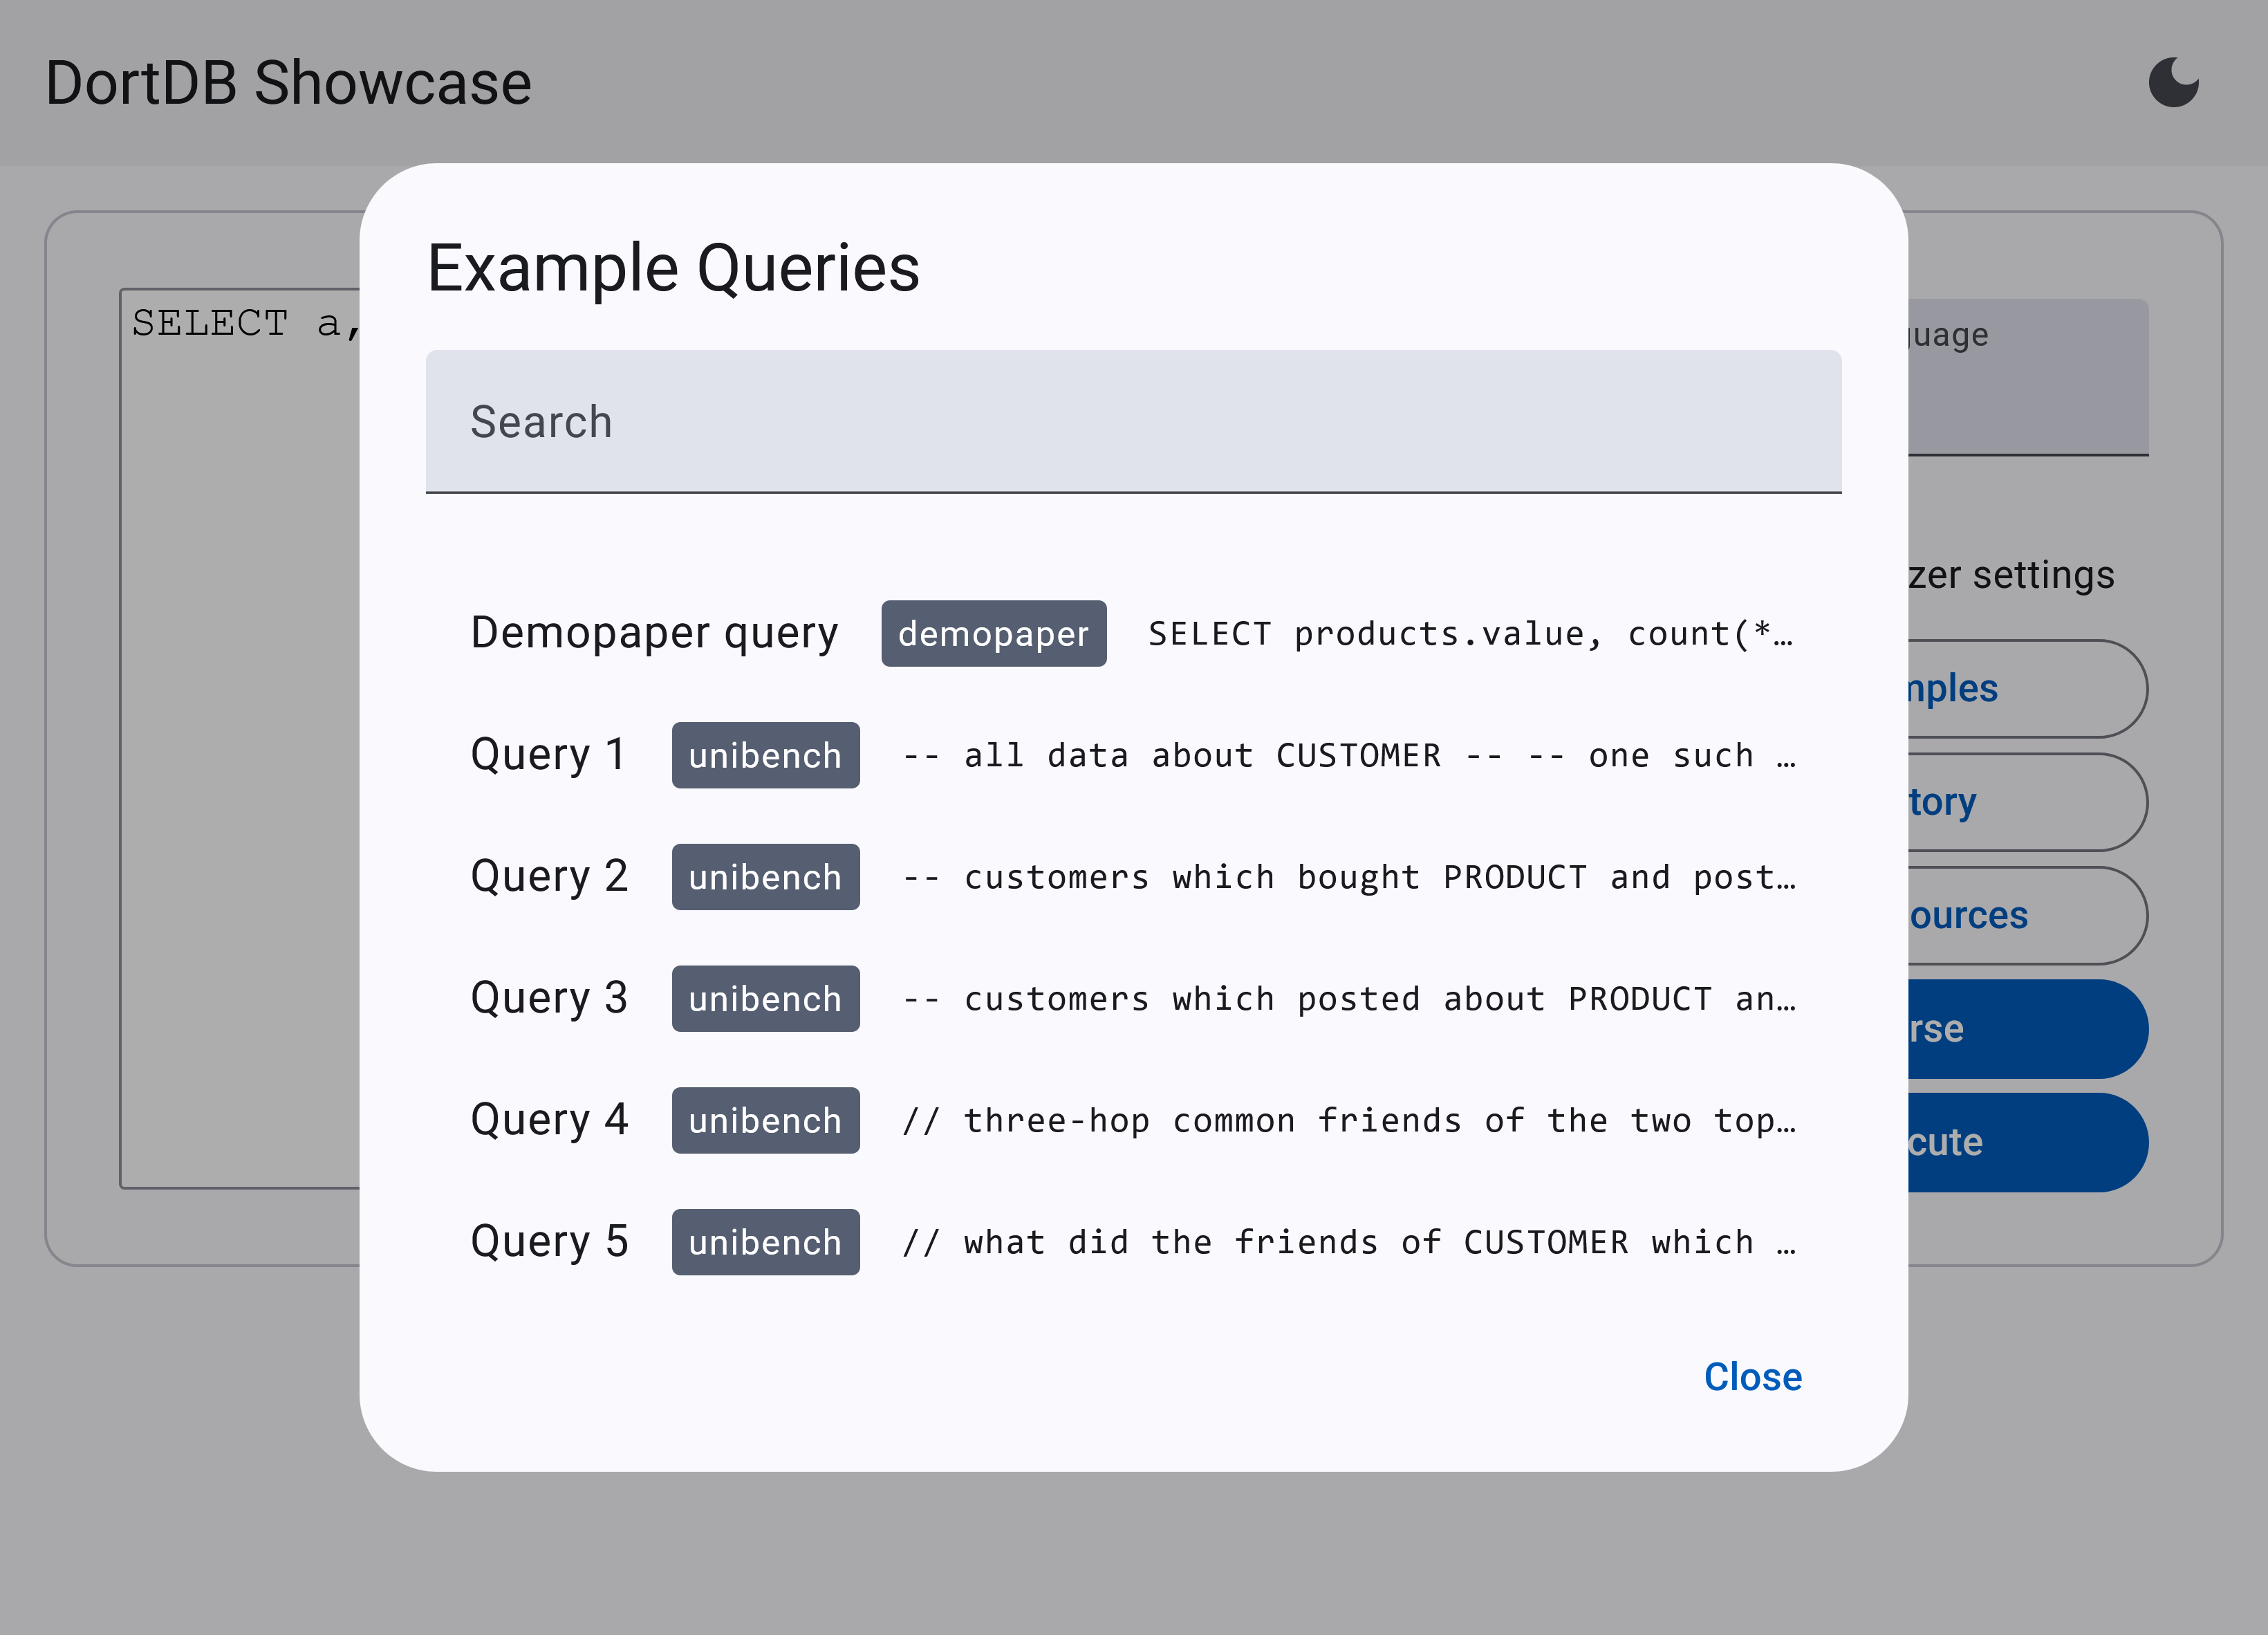
\includegraphics[width=0.8\linewidth]{img/showcase_example_queries.png}
    \caption{Showcase example queries. In order to help the user properly try out DortDB, this dialog offers a quick way to find interesting examples.}
\end{figure}

\begin{figure}[!h]
    \centering
    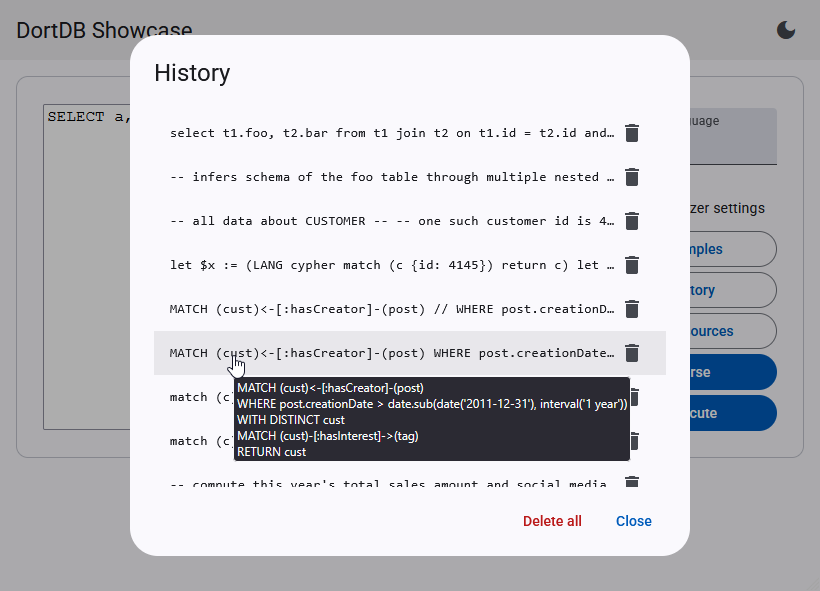
\includegraphics[width=0.8\linewidth]{img/showcase_history.png}
    \caption{Showcase query history. The history remembers the last 20 parsed or executed queries.}
\end{figure}

\begin{figure}[!h]
    \centering
    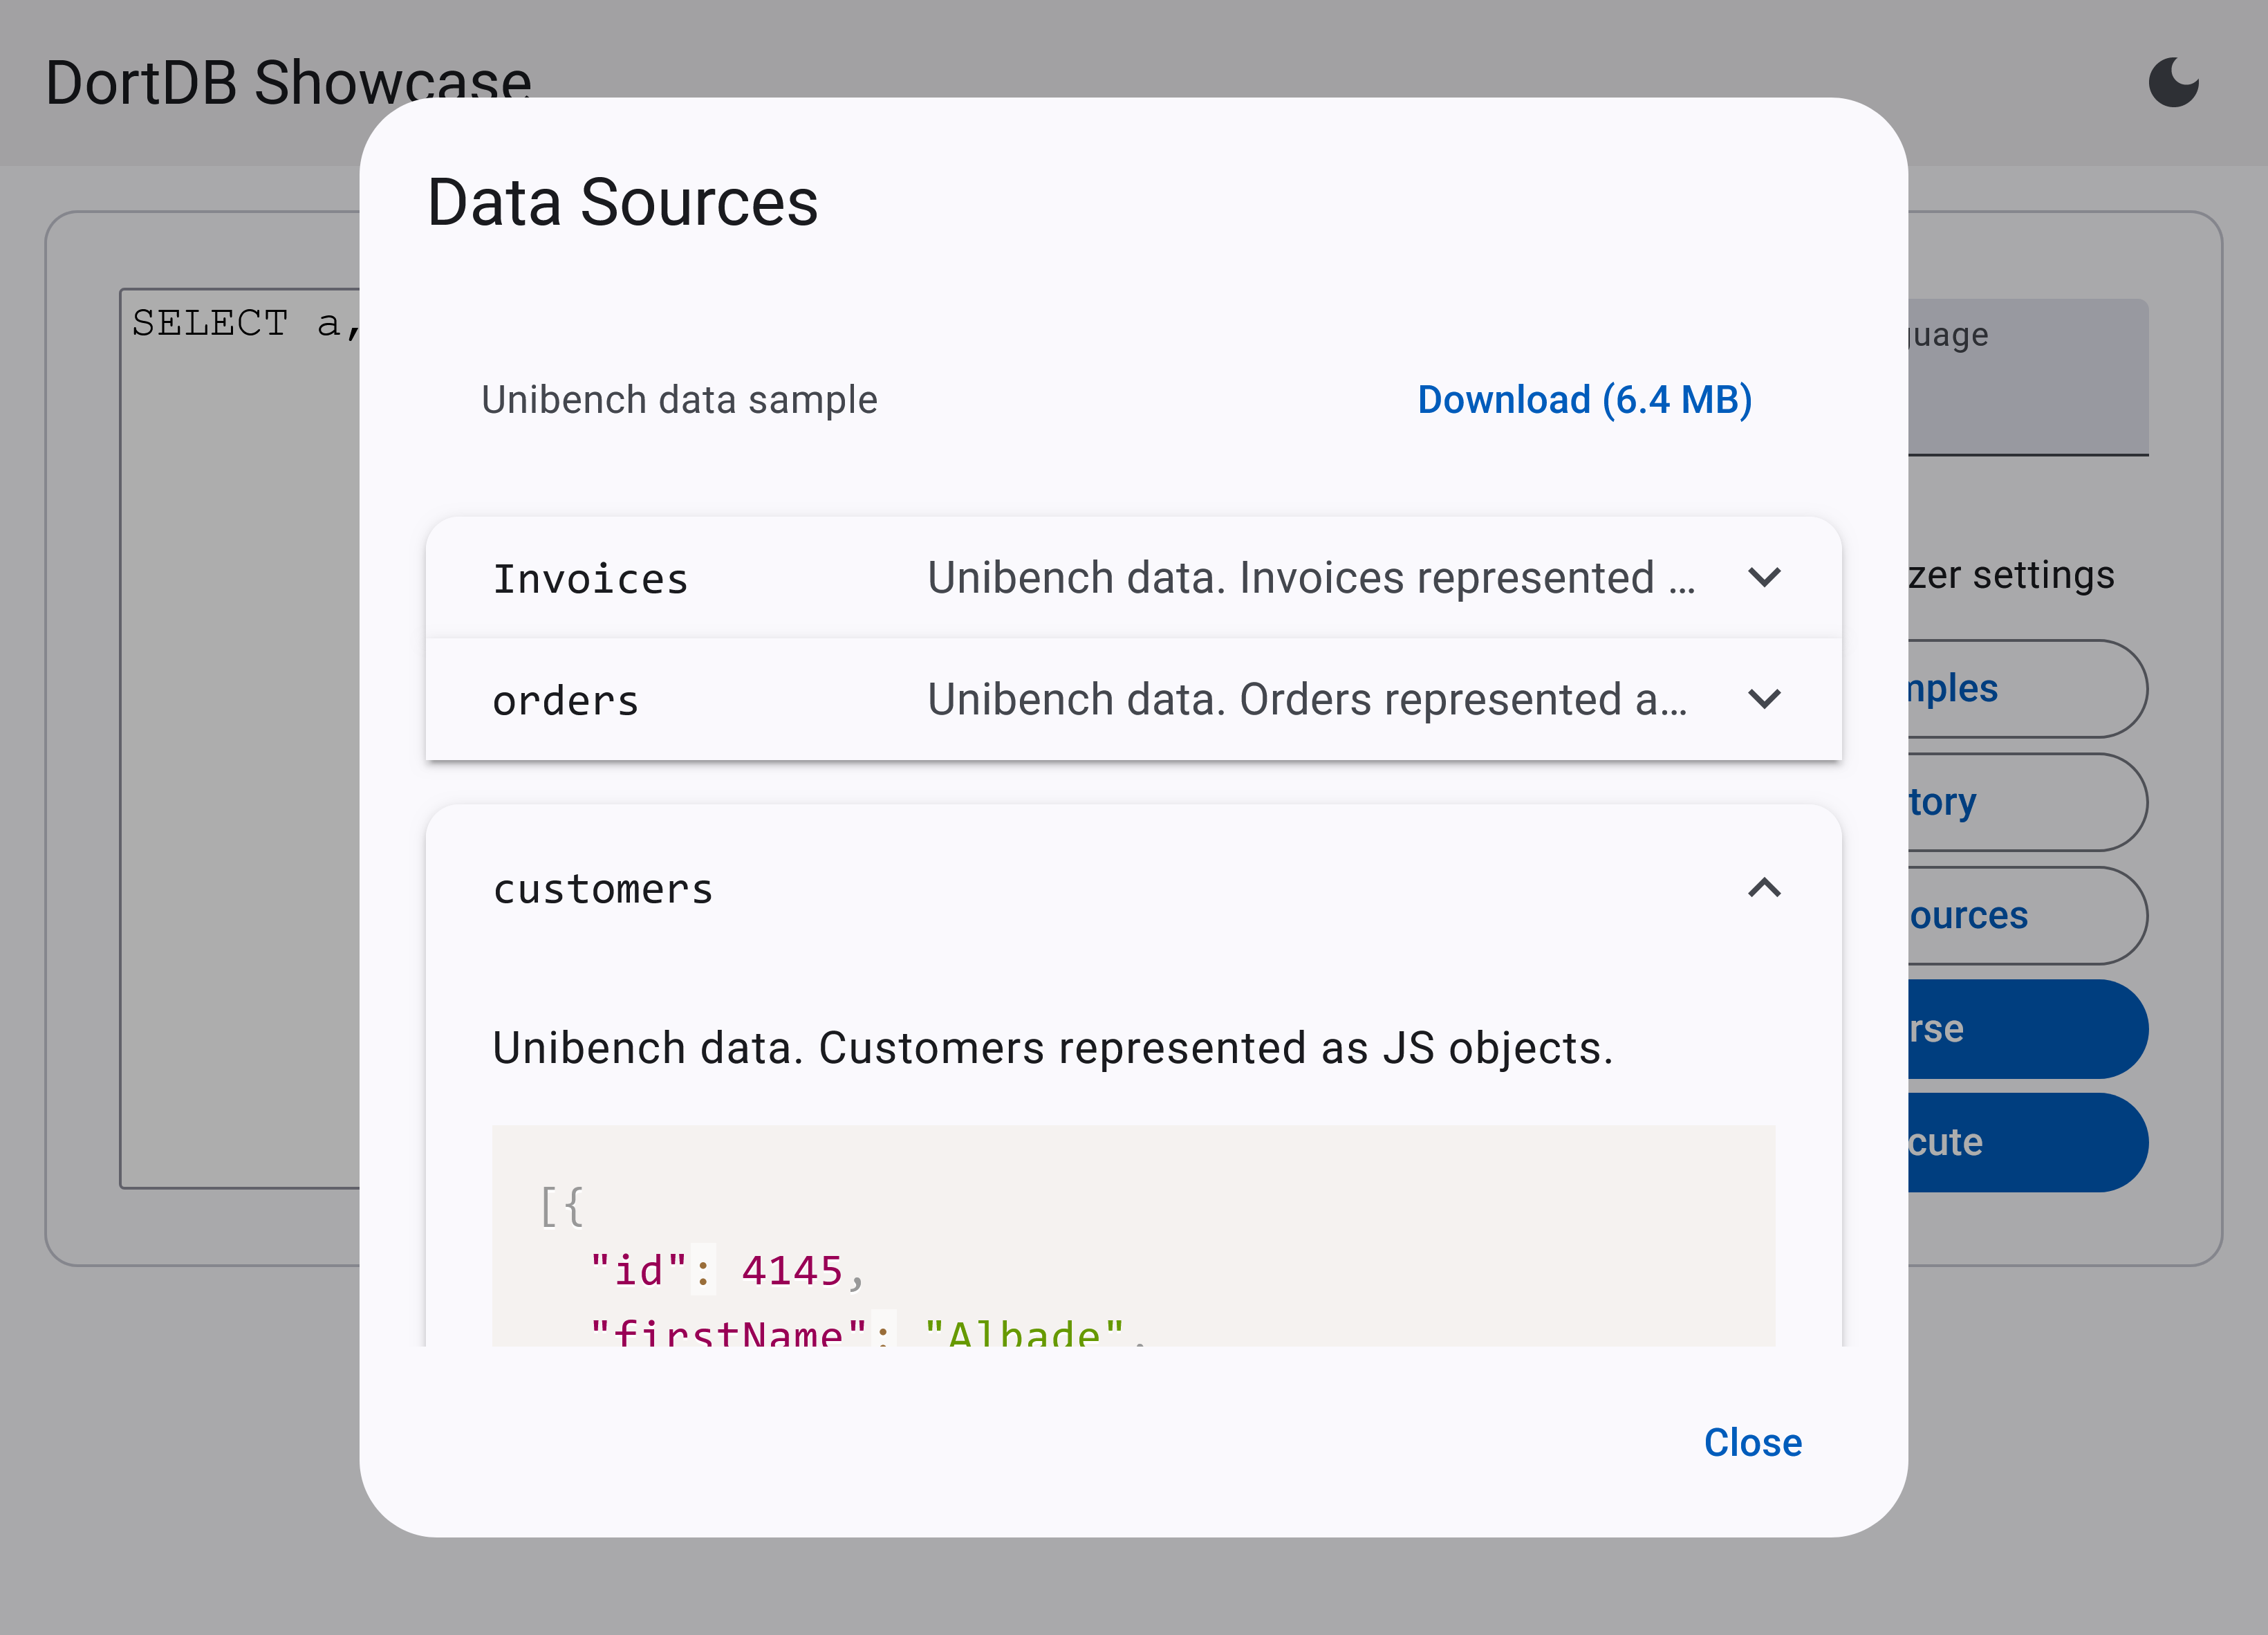
\includegraphics[width=0.8\linewidth]{img/showcase_data_sources.png}
    \caption{Showcase data sources. Showcase allows users to download a sample of the UniBench data and register it as data sources. The individual data sources are described in collapsible expansion panels. Once the user downloads the data, the dialog offers to save the parsed data into the web browser to avoid redownloading it when the page is refreshed.}
\end{figure}

\begin{figure}[!h]
    \centering
    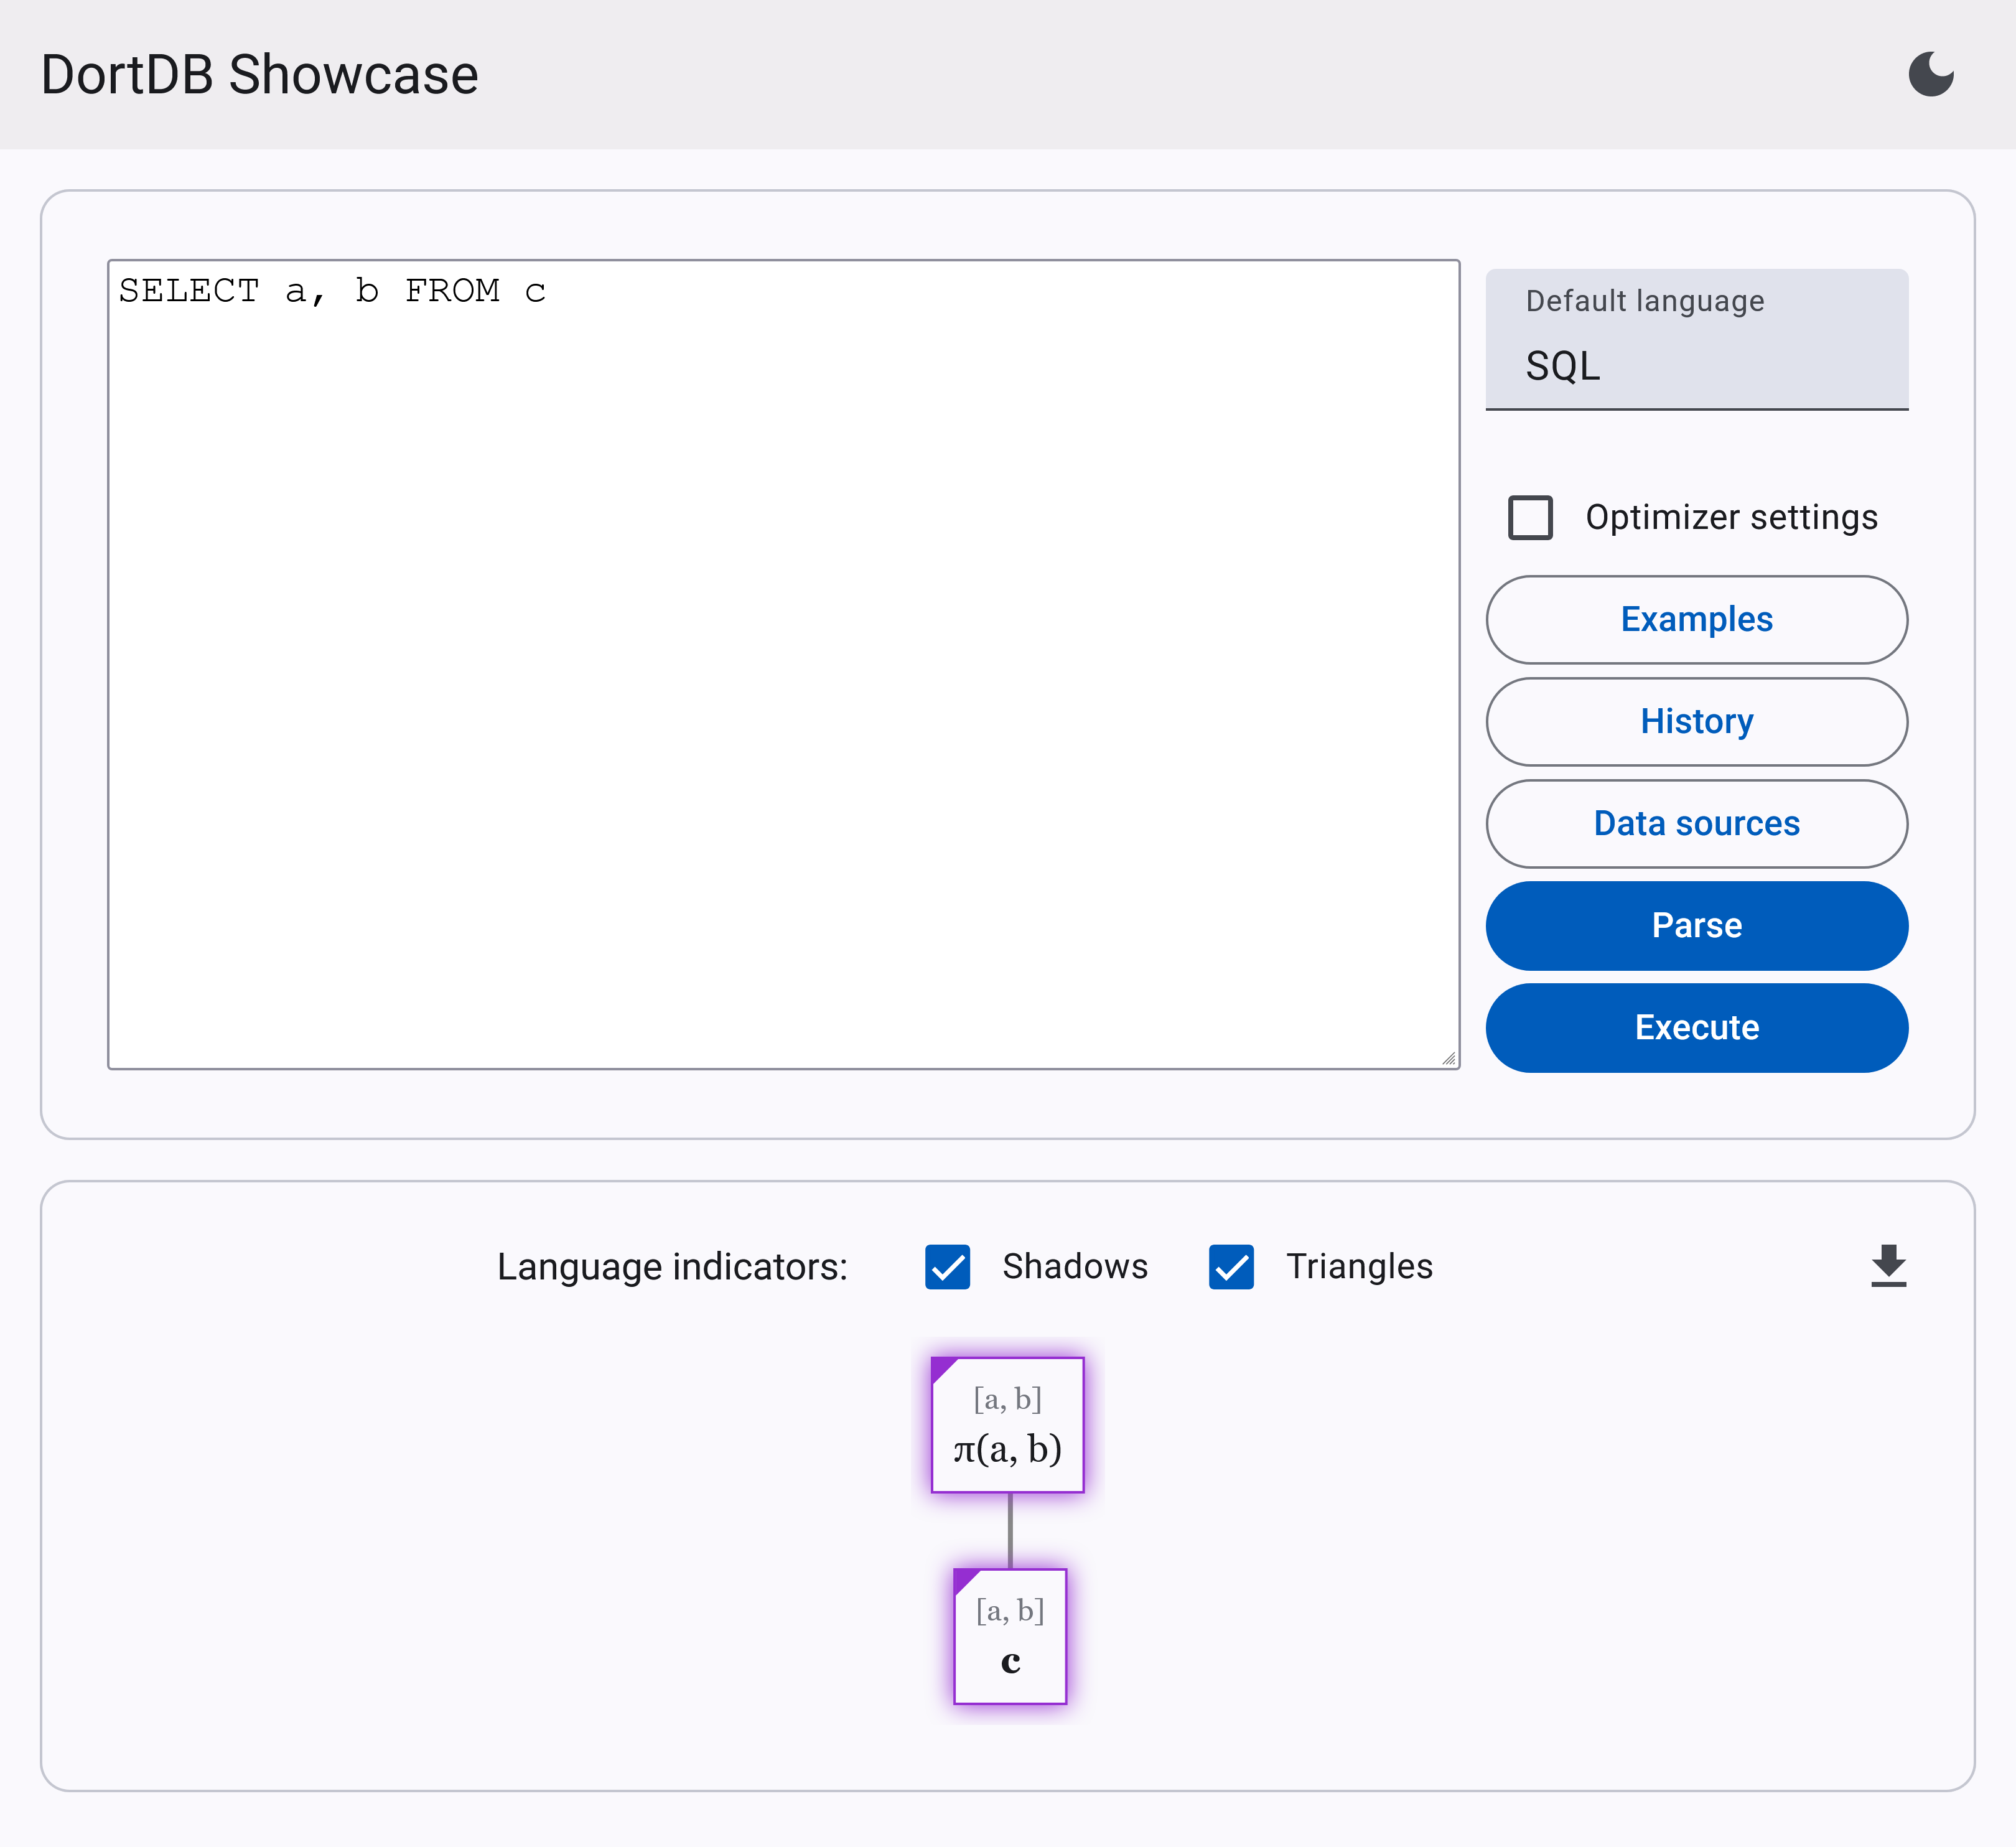
\includegraphics[width=0.8\linewidth]{img/showcase_parse.png}
    \caption{When the query is parsed, the logical plan is displayed as an interactive tree, similar to previous figures in this thesis. The tree can be zoomed and panned. It is possible to download the tree as a PNG image.}
\end{figure}

\begin{figure}[!h]
    \centering
    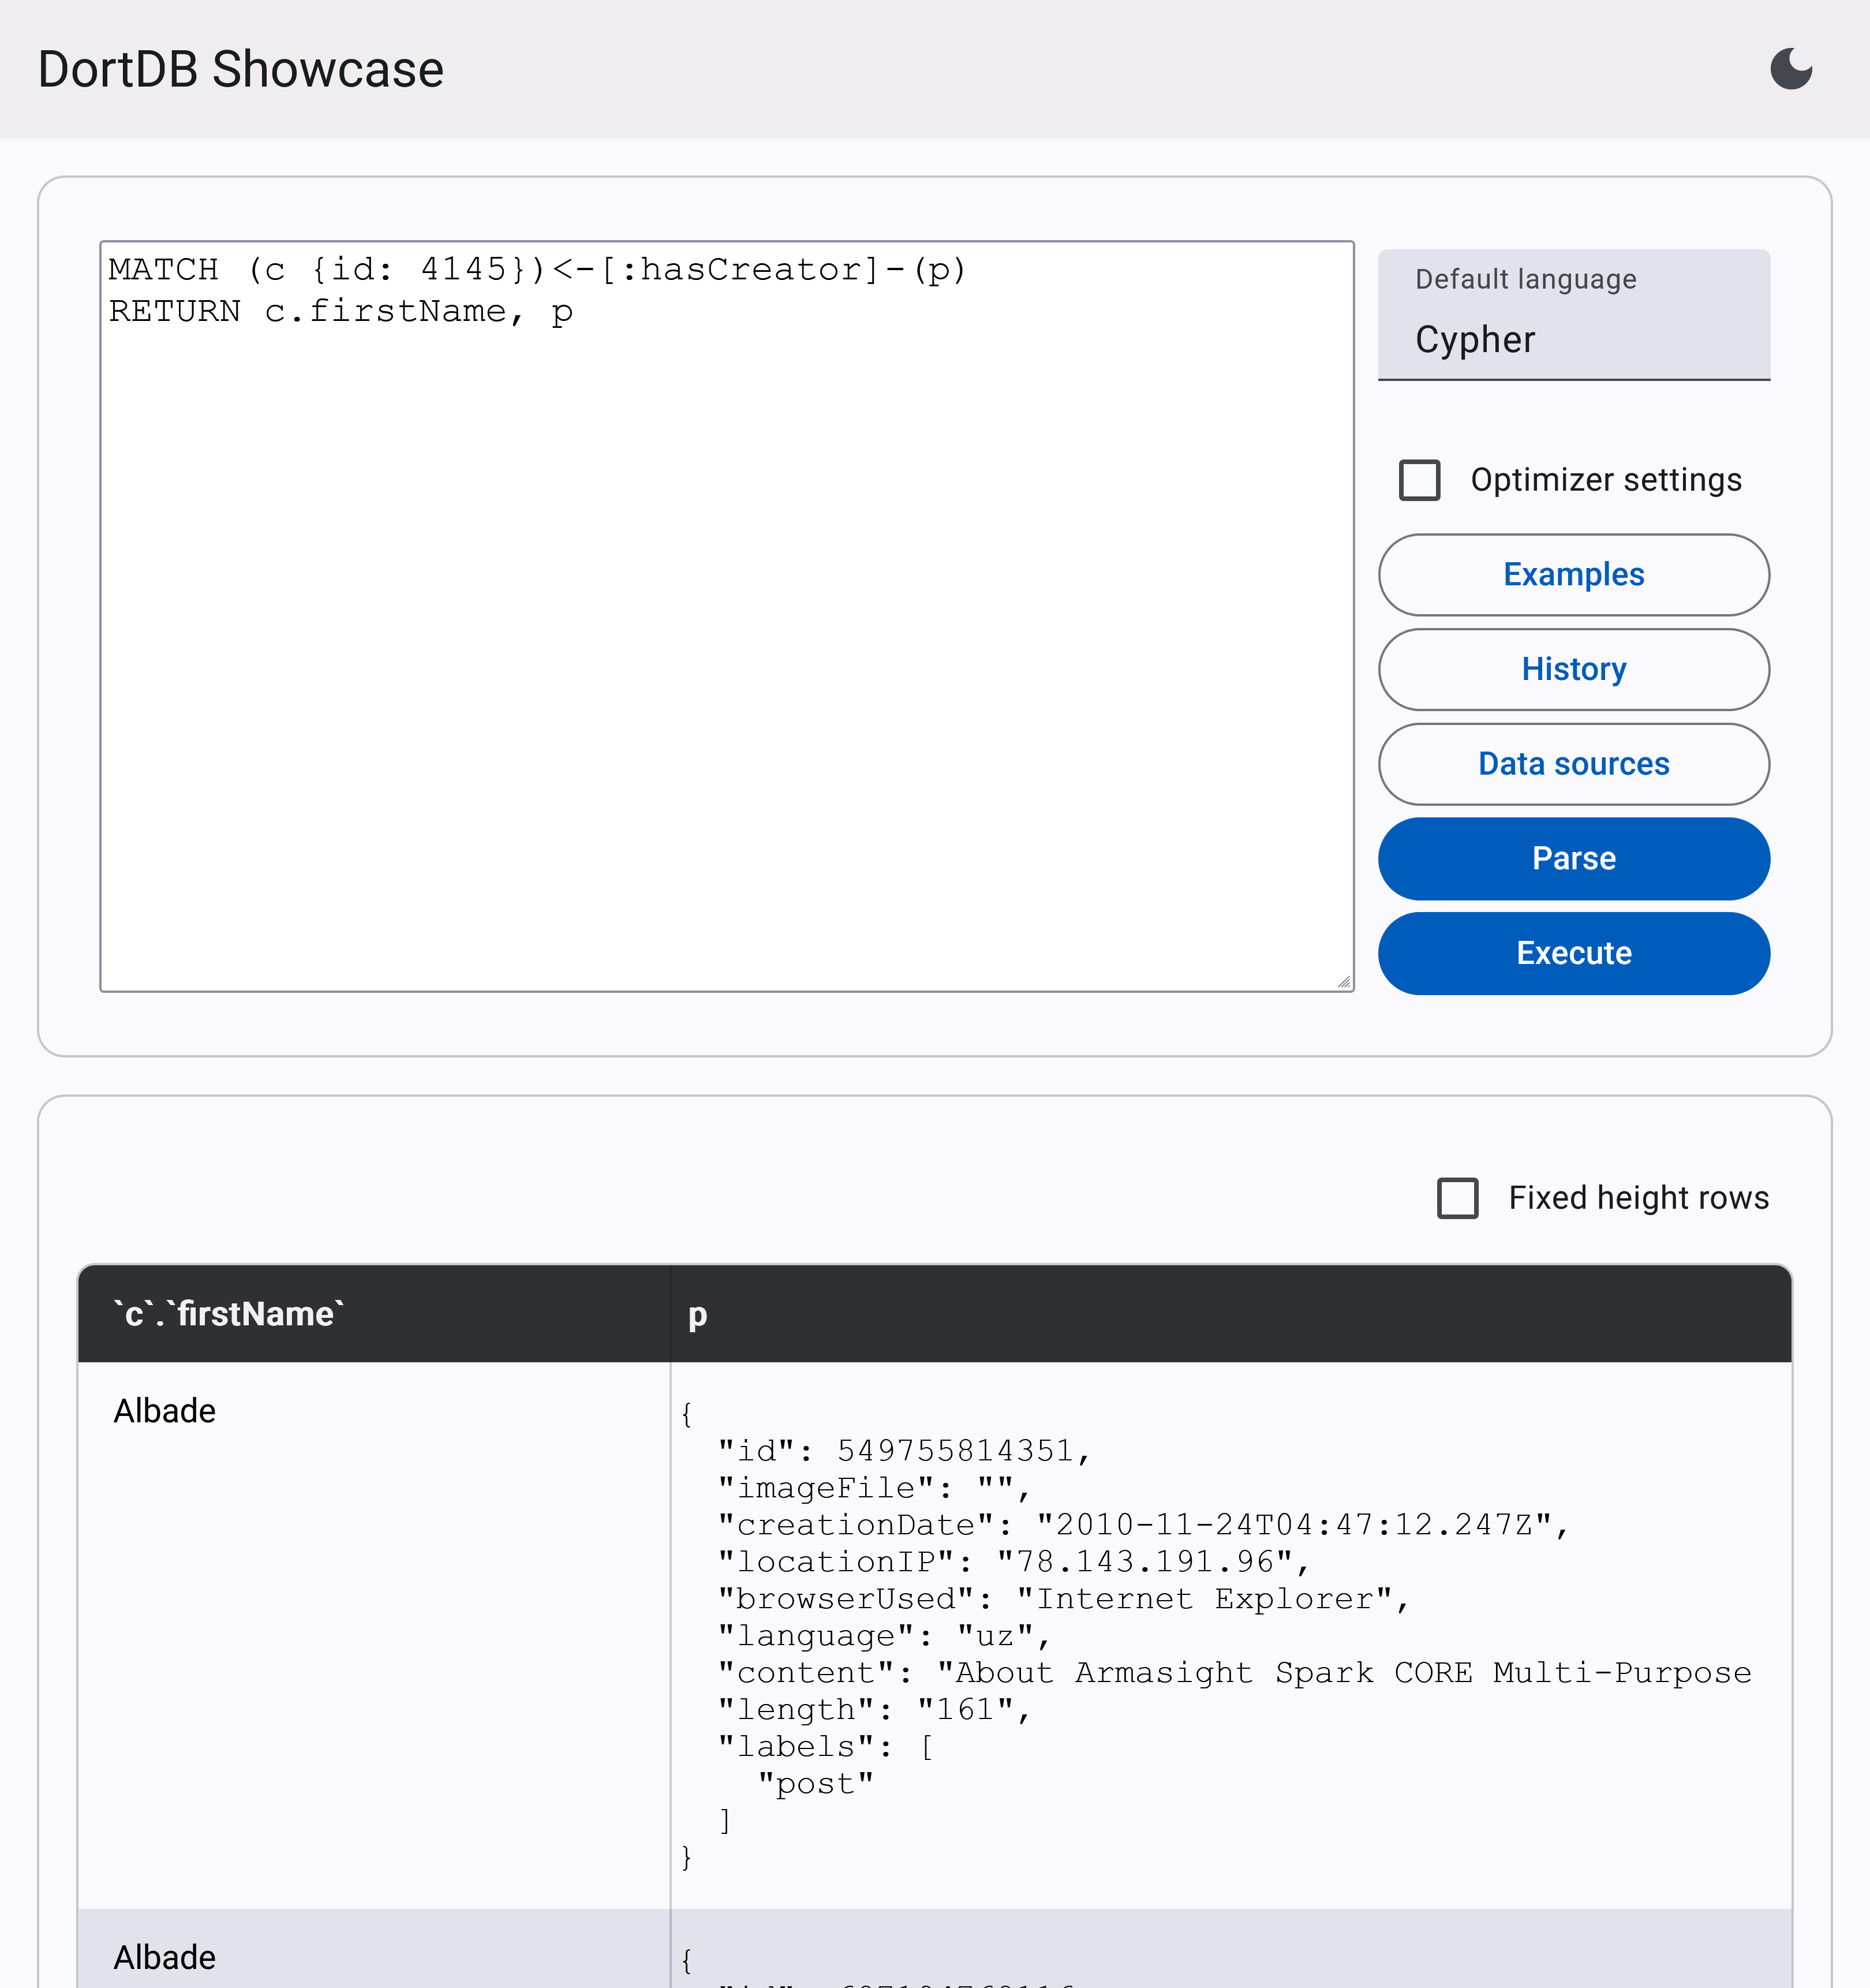
\includegraphics[width=0.8\linewidth]{img/showcase_execute.png}
    \caption{The results of the query execution are displayed in a paginated table. The table columns have adjustable widths.}
\end{figure}

\begin{figure}[!h]
    \centering
    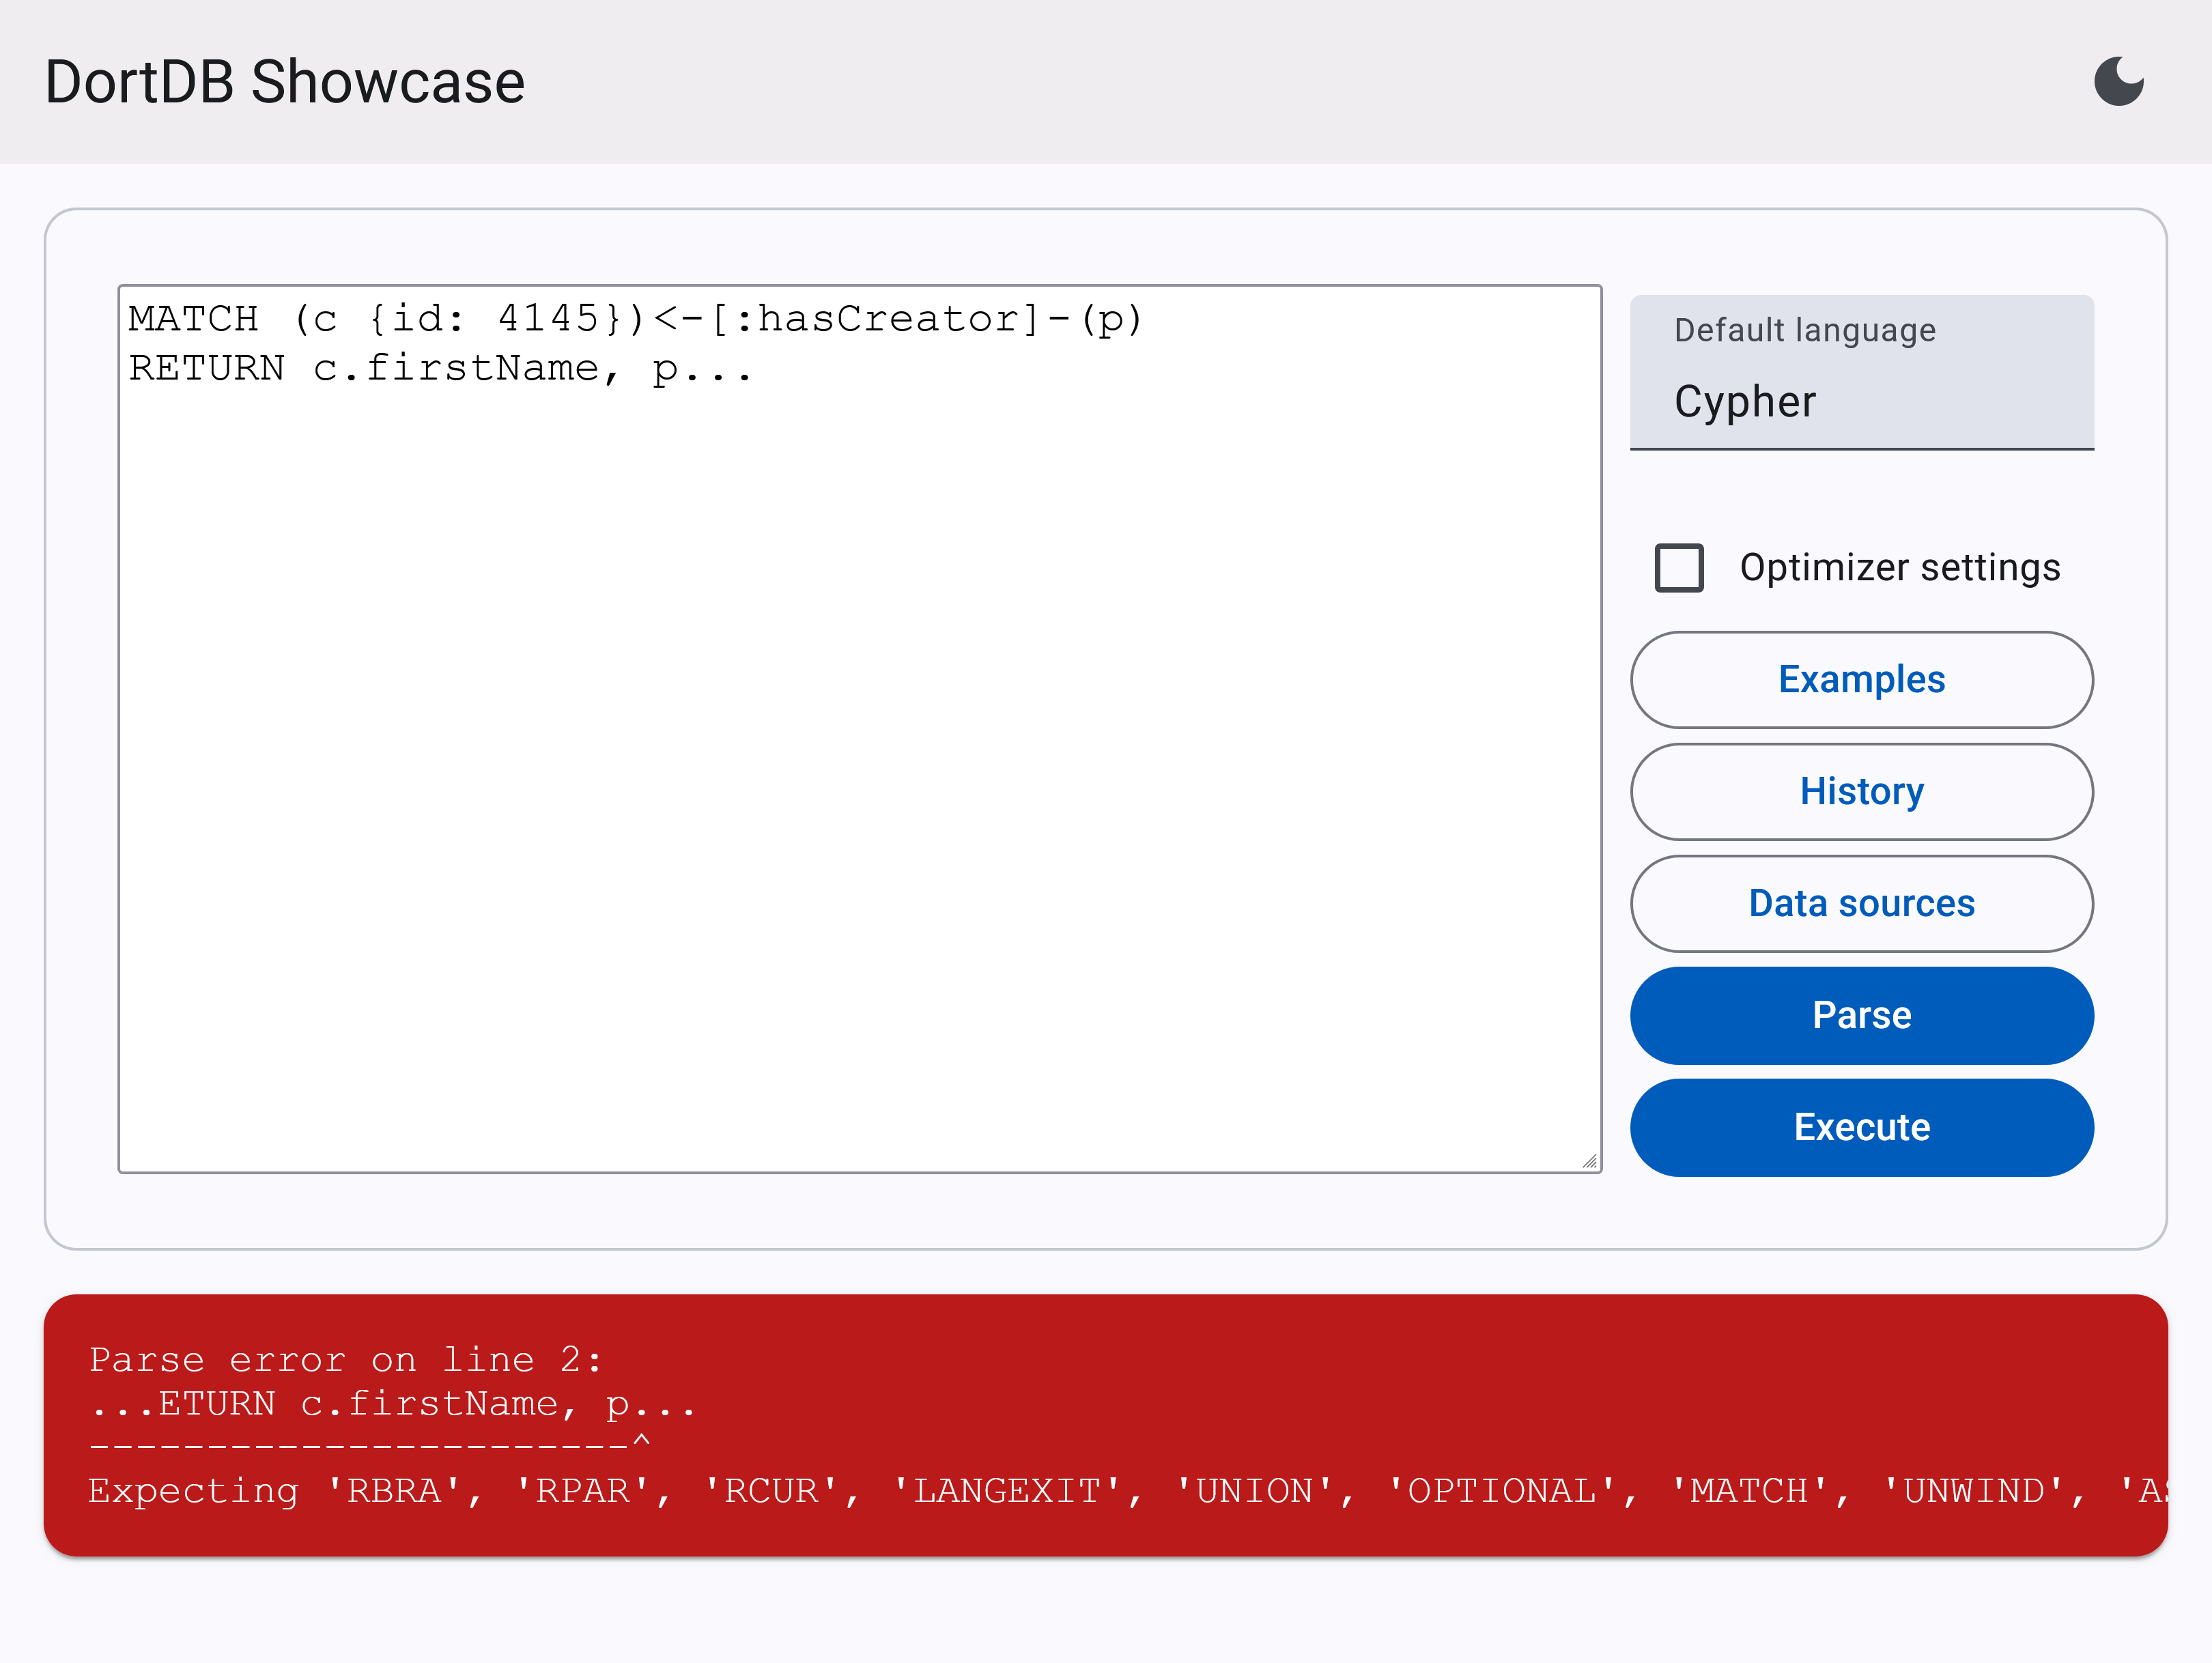
\includegraphics[width=0.8\linewidth]{img/showcase_error.png}
    \caption{Query errors are displayed to the user.}
\end{figure}

\begin{figure}[!h]
    \centering
    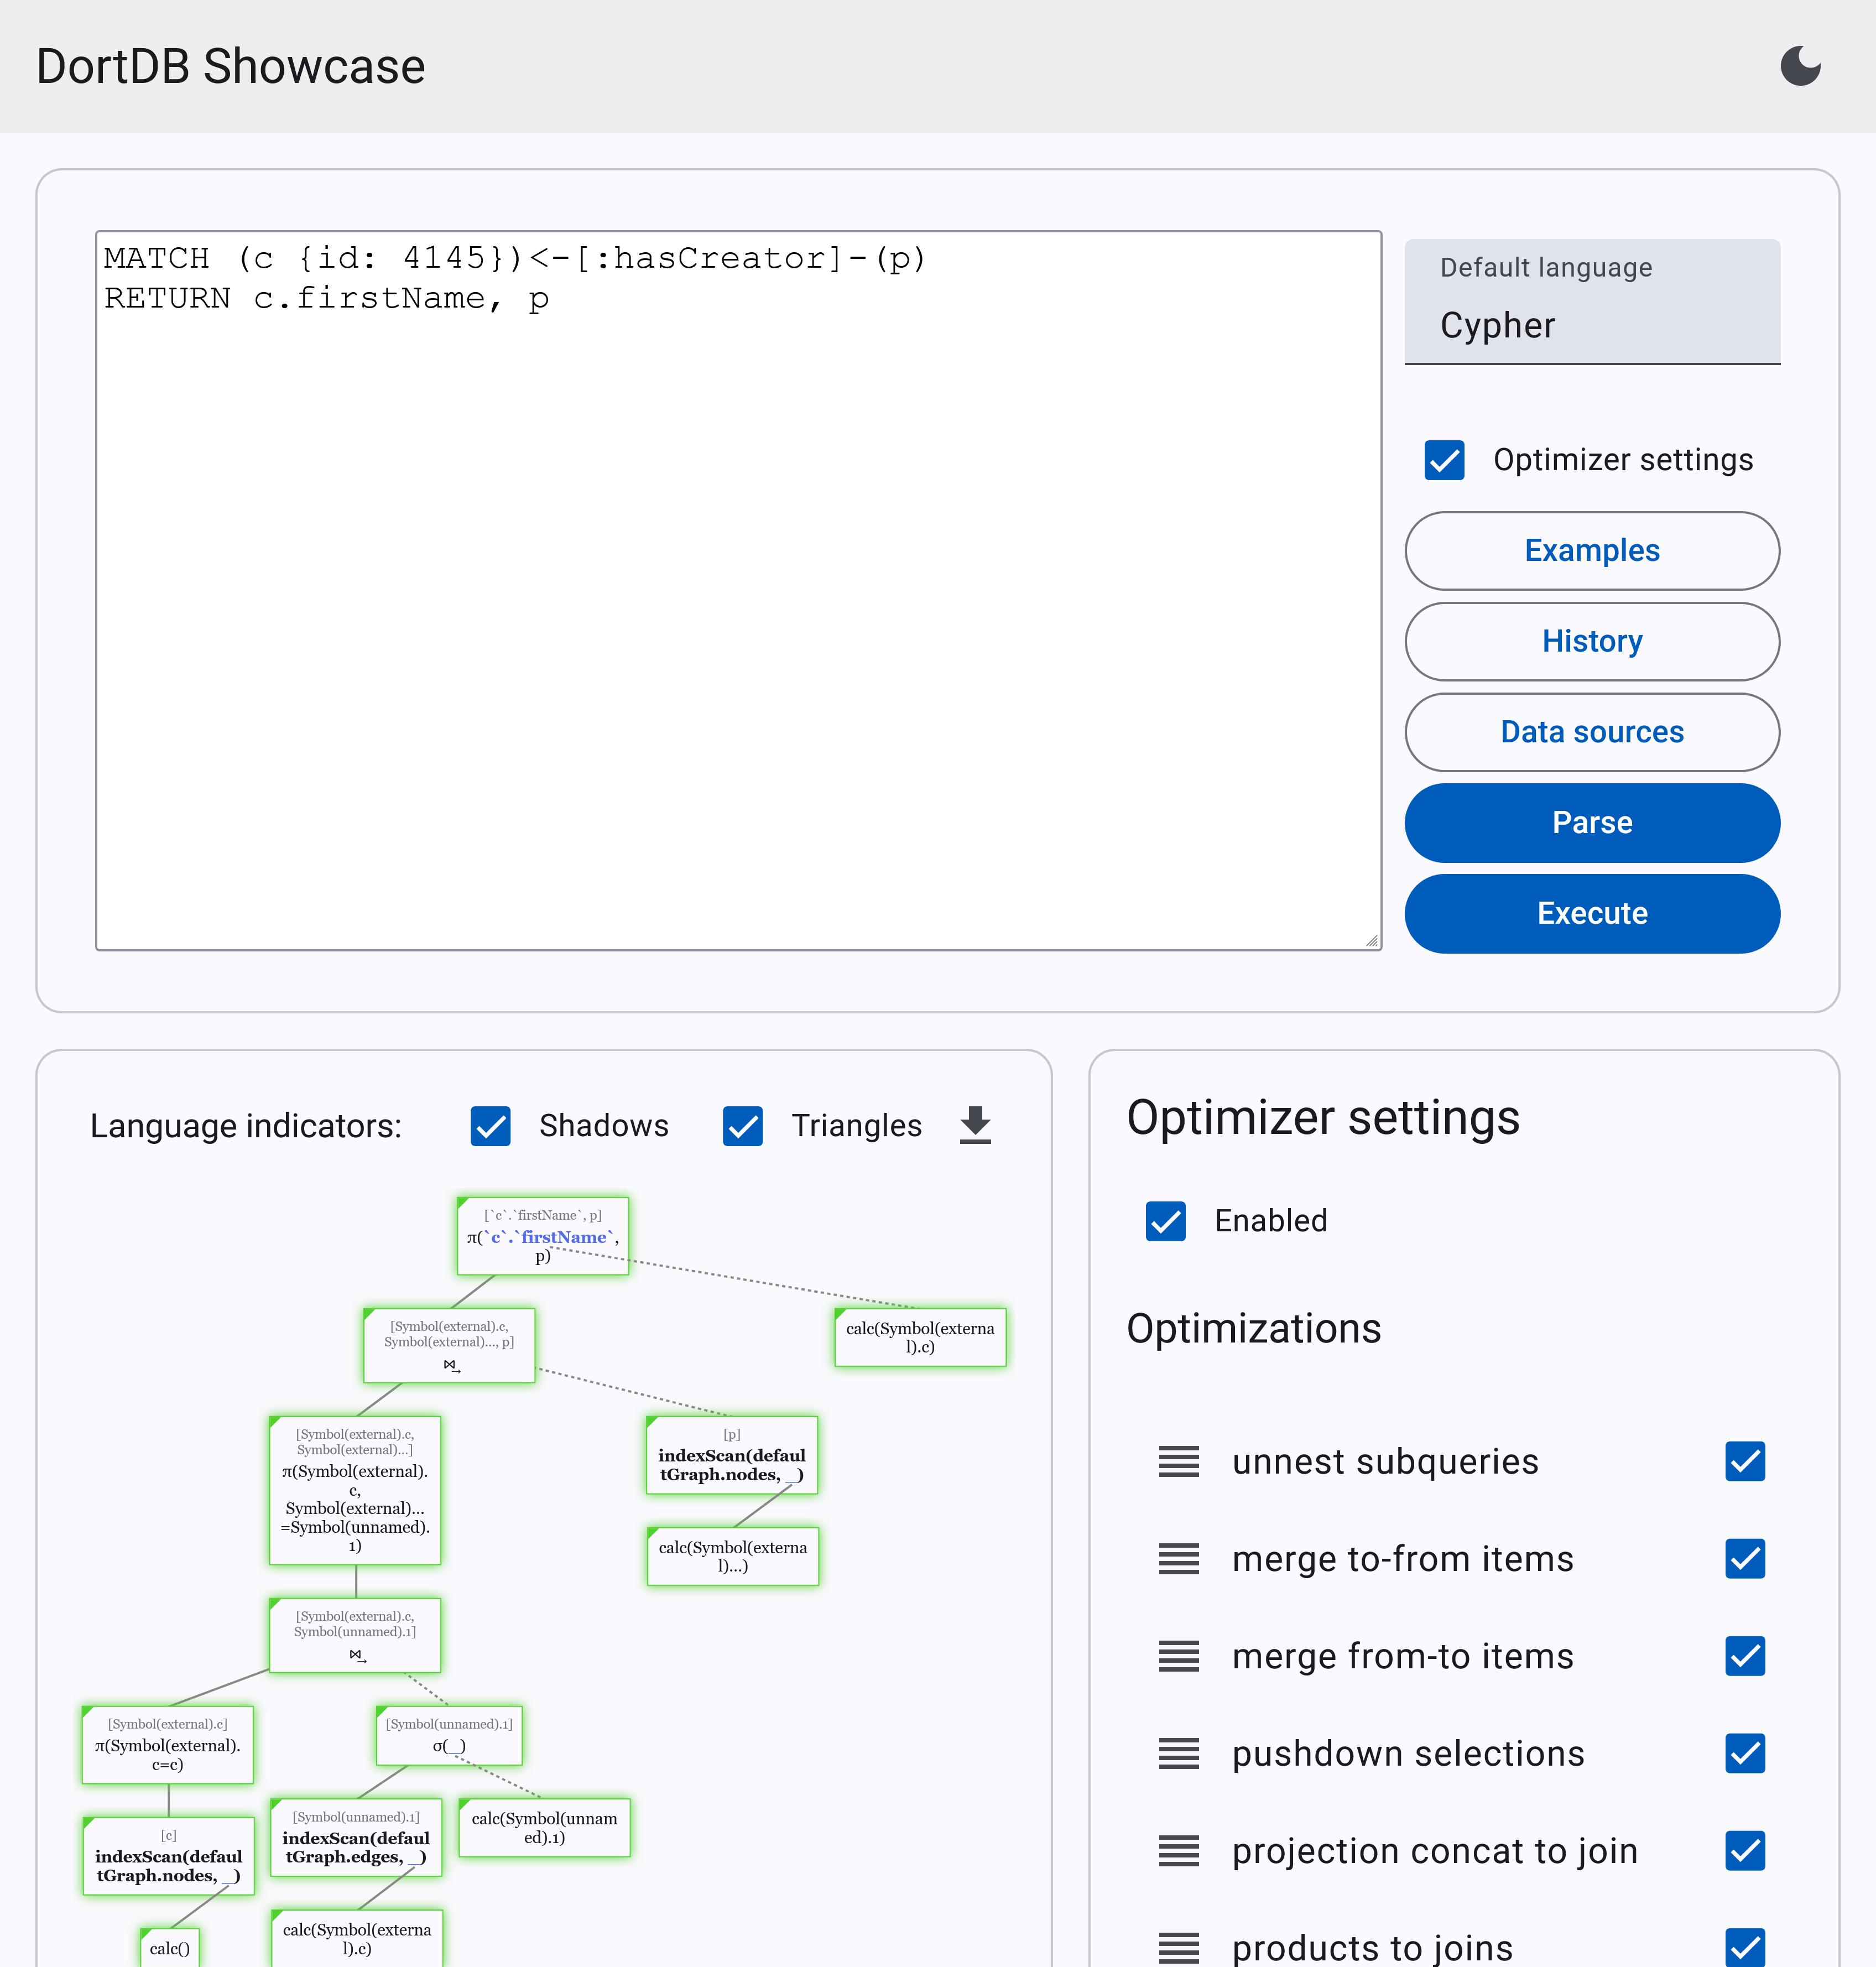
\includegraphics[width=0.8\linewidth]{img/showcase_optimizer.png}
    \caption{Showcase optimizer settings. The optimizer can be completely turned off. It is also possible to disable individual rules or to reorder them using drag \& drop.}
\end{figure}

\clearpage
\section{Programmatic usage}

The main class of the DortDB framework is simply called \texttt{DortDB}. It serves as the container for languages and extensions and exposes methods for registering data sources or querying. When creating a \texttt{DortDB} instance, it is necessary to provide at least one language. In order to facilitate better tree shaking, the optimizer, by default, receives no rules. However, all currently available rules are exported in a single array, already ordered for best performance. The individual languages can also be configured, for example, to use a different data adapter. The DortDB configuration can also specify additional user-defined functions, operators, or aggregates. It is also possible to bundle functions, operators, and aggregates into a single importable object called an extension. DortDB already comes with a \texttt{datetime} extension for manipulating dates and times. Extensions can be scoped to specific languages only. Only some languages support user-defined operators, for example, SQL.

\begin{listing}[!ht]
\begin{minted}{ts}
import { datetime, DortDB } from '@dortdb/core';
import { defaultRules } from '@dortdb/core/optimizer';
import { SQL } from '@dortdb/lang-sql';
import { DomDataAdapter, XQuery } from '@dortdb/lang-xquery';
import { Cypher } from '@dortdb/lang-cypher';

const db = new DortDB({
  mainLang: SQL(),
  additionalLangs: [
    XQuery({
      // in browser environment
      adapter: new DomDataAdapter(document)
    }),
    Cypher({ defaultGraph: 'defaultGraph' })
  ],
  optimizer: {
    rules: defaultRules,
  },
  extensions: [
    datetime,
    {
      scope: ['cypher'],
      aggregates: [
        // ... aggregates only for Cypher
      ],
    },
  ],
});
\end{minted}
\caption{DortDB data sources registration.}
\end{listing}

Once a \texttt{DortDB} instance is created, data sources can be registered. All the registration does is a pairing of a data structure with an identifier. It is then possible to index the structure with secondary indices. The developer needs to specify which type of index is used.

\begin{listing}[!ht]
\begin{minted}[fontsize=\small]{ts}
import { MapIndex } from '@dortdb/core';
import { MultiDirectedGraph } from 'graphology';

// db is already initialized
const arr = [1, 2, 3];
const obj = { prop: 'value' };
const objArr = [obj];

// the identifiers can have multiple parts
db.registerSource(['testing', 'arr'], arr);
db.registerSource(['testing', 'objArr'], objArr);
// anything can be registered, it is up to 
// the language data adapters to use it
db.registerSource(['testing', 'obj'], obj);
db.registerSource(['defaultGraph'], new MultiDirectedGraph());

// a simple hash index
// some indices may support indexing multiple expressions
db.createIndex(['testing', 'objArr'], ['prop'], MapIndex);
// the indexed expression is parsed with the default language
// but this can be changed by passing in a config parameter
db.createIndex(['testing', 'objArr'], ['prop->2'], MapIndex);

// for data sources that should be interpreted as item sources
// a specific identifier is configured to be treated as the item
// while parsing the expression
db.createIndex(['defaultGraph', 'nodes'], ['x.id'], MapIndex, {
  mainLang: 'cypher',
  fromItemKey: ['x'],
});
\end{minted}
\caption{DortDB initial setup.}
\end{listing}

\begin{listing}[!ht]
\begin{minted}[fontsize=\small]{ts}
import { UnnestSubqueries } from '@dortdb/core/optimizer';

db.optimizer.reconfigure({
  rules: [UnnestSubqueries]
});
\end{minted}
\caption{The query optimizer can be reconfigured at any time.}
\end{listing}

After the database is fully configured, we can parse queries into an AST, build and optimize logical plans, and execute them. Both the AST and the logical plan implement the visitor design pattern, so additional preprocessing can be added. All of the logical plan operators also expose a \texttt{getChildren()} method, so it is possible to quickly and simply iterate through the whole operator tree.

\begin{listing}[!ht]
\begin{minted}[fontsize=\small]{ts}
import { ASTNode } from '@dortdb/core';
import * as plan from '@dortdb/core/plan';

const query = 'SELECT a FROM t';

// some languages allow multiple statements
// per one query, so the result is an array
const ast: ASTNode[] = db.parse(query);

const plan = db.buildPlan(ast.at(-1));

// if we wanted to invert `orderBy` directions, we
// could write a visitor, or do it the quick way:
const stack = [plan];
while (stack.length) {
  const current = stack.pop();
  stack.push(...current.getChildren());
  if (current instanceof plan.Order) {
    for (const o of current.orders) {
      o.ascending = !o.ascending;
    }
  }
}

const results = db.executePlan(plan);

// during the relevant phases, the default language
// can be changed, and bound parameters can be provided

// we can also just query without caring about the plan or AST
const newResults = db.query(`
  MATCH (a)-[]->(b)
  WHERE a.id > $id
  RETURN a, b
`, {
  mainLang: 'cypher',
  boundParams: { id: 13 }
});
\end{minted}
\caption{Querying the database.}
\end{listing}

\section{Extensibility}
\label{sec:usage-extensibility}

One of DortDB's main selling points is its extensibility. It is possible (and encouraged) to provide more languages, index types, optimizer rules, or extensions. This section aims to outline in broad steps how to do all of the above-mentioned.

\subsection{Authoring a new language}

First of all, it is necessary to implement a parser that will parse the language queries into an AST. The parser must recognize language switches and switch to a different parser and then resume parsing afterward. To this end, each parser must recognize when to end even if there is yet remaining input, be it because of an encountered \texttt{LANG EXIT} token or because the parser would exit its initial scope. The parser should return both the parsed AST and any remaining unparsed input, so that an outer parser could continue, as in Program \ref{fig:parser-exit}.

\begin{listing}[!ht]
\begin{minted}{sql}
SELECT t1.attr1 FROM (
  LANG newlang
  -- new language here...
) AS t1 WHERE attr1 > 3
\end{minted}
\caption{The nested language should recognize the closing parenthesis as a scope exit and terminate. It should return both the parsed AST and the remaining input string \mintinline{sql}{) AS t1 WHERE attr1 > 3}.}
\label{fig:parser-exit}
\end{listing}

After the AST is available, the language should build an initial logical plan. If the unified algebra does not suffice, the language can define its own plan operators. It must, however, extend all core visitors to take these new operators into account. When building the plan, the language will receive an \texttt{IdSet} with identifiers defined in the outer context. Some of the identifiers in the \texttt{IdSet} may have the \texttt{Symbol(toInfer)} as their last token. This means that the identifier belongs to a data source whose schema is still being inferred. If the language encounters any matching identifiers, it should record them and return them in addition to the built logical plan.

\begin{listing}[!ht]
\begin{minted}[fontsize=\small]{ts}
import { AttributeRenamer, PlanVisitor } from '@dortdb/core';
import { TreeJoin, XQueryPlanVisitor } from '../plan/index.js';
import { RenameMap } from '@dortdb/core/plan';

export class XQueryAttributeRenamer
  extends AttributeRenamer
  implements XQueryPlanVisitor<void, RenameMap>
{
  // ...
  visitTreeJoin(operator: TreeJoin, renames: RenameMap): void {
    operator.source.accept(this.vmap, renames);
    this.processItem(operator, 'step', operator.dependencies, renames);
  }
}

// in language.ts:

export function XQuery(config?: XQueryConfig): XQueryLanguage {
  return {
    name: 'xquery',
    // ...
    visitors: {
      attributeRenamer: XQueryAttributeRenamer,
      // ...
    },
  };
}
\end{minted}
\caption{When extending the unified algebra, all core visitors must be extended as well. This example is taken from \texttt{@dortdb/lang-xquery}.}
\end{listing}

\subsection{Authoring a new index type}

DortDB features secondary indices. The index must implement the following three methods: \texttt{match}, to receive an array of expressions and decide whether some match the index. \texttt{CreateAccessor}, which takes an array of expressions that match the index, and should return a \texttt{calculation} which accesses the index and finds matching items for specific values of the expressions. Finally, there is the \texttt{reindex} method, which receives items from the connected data source and values of the indexed expressions, and should fill the index data structure.

The index does not always need to store the data in any structure. For example, the Cypher \texttt{ConnectionIndex} detects join conditions between nodes and edges, and then selects connected edges or nodes using the Cypher data adapter.

\subsection{Authoring other components}

Besides entire languages or specialized secondary indices, DortDB can also be extended with new optimizer rules. This may be especially relevant for custom logical plan operators. The rules may be as simple as removing neighboring \texttt{mapFromItem} and \texttt{mapToItem}, or complex algorithms for merging \texttt{Projections}. In all cases, they can be reduced to two methods: \texttt{match}, which recognizes patterns in the logical plan, and \texttt{transform}, which replaces the patterns with other patterns.

Finally, DortDB users may define their own functions or aggregates. These may be grouped into and distributed as extensions, for example, for spatial data manipulation or for the creation of dynamic data sources.
\chapter{Related work}
\label{chap:related-work}

Now that we have established DortDB, evaluated its performance, and seen its user interface and programmer interface, we can properly compare it with existing solutions. First, we will compare DortDB to other multimodel database systems. Then, we will inspect a dramatically different approach to universal multimodel queries. Lastly, we will examine leading in-memory JavaScript databases.

\section{ArangoDB}

ArangoDB\footnote{\url{https://arangodb.com/multi-model-db/}} is a highly popular multimodel database. Its base data model is a graph, but it also supports vector data, as well as hierarchical document data, key-value, or full-text search. ArangoDB features its own query language called AQL, which can seamlessly combine all of the mentioned data models. Its query optimizer is very powerful, as evidenced by our benchmarks. DortDB is outmatched in all regards. The only edge DortDB might have is the possibility that if a new data model emerged, DortDB could incorporate it in a more straightforward way.

\begin{listing}[!ht]
\begin{minted}{text}
LET personlist = (
  FOR post IN INBOUND CONCAT("Product/", @key) PostHasTag
  FOR person IN INBOUND post._id PersonHasPost
  LIMIT 100
  RETURN person._key
)
FOR order IN Order
FILTER order.OrderDate > "2022"
AND @key IN order.Orderline[*].productId
AND order.PersonId IN UNIQUE(personlist)
RETURN DISTINCT(order.PersonId)
\end{minted}
\caption{Example of an AQL query. It is the ArangoDB version of UniBench query 2. It selects customers who have bought a specific product and posted about it. The query combines graph and document models.}
\end{listing}

\section{OrientDB}

OrientDB\footnote{\url{https://orientdb.dev/}} is an open-source document and graph database. It claims to be the first multimodel database in the world. It offers tools for ETL (extract, transform, load) pipelines. While we were unable to import the UniBench data into the most recent version of OrientDB, we have tested the performance of an older build. This time, DortDB comes close in some specific queries, as OrientDB is not optimized for relational workloads. Compared to DortDB, OrientDB is less flexible and harder to initially set up. It is, however, much more powerful when it comes to graph queries. It uses an extended version of SQL without joins.

\begin{listing}[!ht]
\begin{minted}[ignorelexererrors=true]{sql}
SELECT $person
LET $list = (
  SELECT IN('PostHasTag').IN('PersonHasPost').id AS pid
  FROM `Product`
  WHERE productId = :id
), $person = (
  SELECT PersonId, Orderline.productId
  FROM Order
  WHERE OrderDate > "2022"
  AND PersonId IN $list
  AND :id IN Orderline.productId
)
\end{minted}
\caption{The same query written in OrientDB SQL.}
\end{listing}

\section{MMQL}

Our approach to universal querying of multimodel data is to combine suitable languages as necessary, combining them all into a unified algebra. Arguably, a more intuitive approach is to design a query language that could query anything regardless of its data model. MMQL\cite{DBLP:journals/is/KoupilCH25} is a multimodel query language based on category theory. Practically, it is based on SPARQL syntax, where SPARQL is a graph query language developed for querying linked data. The implemented proof of concept parses the query into multiple model-specific queries, which are dispatched to connected database systems. MMQL then combines the results, joining data and handling data redundancies. The proposed approach bears similarities to polystores, but it aims to be universal in its support of existing database systems and data models.

DortDB and MMQL solve the same problem in opposite ways: MMQL uses a single language and multiple storage systems, while DortDB stores all of the data in one place and queries it with multiple languages at once. DortDB's approach is possible mainly because DortDB keeps all of the data in main memory, and thus does not need to consider storage methods most suited for specific data models. The main advantage of DortDB is that no mapping of the underlying data to the category model is necessary. On the other hand, MMQL can leverage existing highly performant systems, leading to much better performance.


\begin{listing}[!ht]
\begin{minted}[ignorelexererrors=true]{sparql}
SELECT {
  ?customer ordered ?productName ;
    name ?customerName .
}
WHERE {
  ?product 49 ?productName ;
    -39/36 ?order .

  ?order -23/21 ?customer .
  ?customer 3 ?customerName .

  FILTER(?productName = "Lord of the Rings")
}
\end{minted}
\caption{Example of a query written in MMQL, taken from the original thesis\cite{DBLP:journals/is/KoupilCH25}.}
\end{listing}

\section{AlaSQL}

AlaSQL\footnote{\url{https://github.com/AlaSQL/alasql}} is an open-source in-memory SQL database for JavaScript. It comes with a large number of various features. It supports most of the SQL-99 standard, includes syntax for interacting with JSON documents, and a limited form of graph queries. It allows the developer to query existing data structures and to define custom functions and aggregates. It is also possible to query and modify data stored in XLSX, CSV, or JSON files.

On the other hand, the addition of many of these features seems to have been haphazard. This resulted in code that is hard to maintain or extend and that is not very performant outside of relatively simple queries. The query plans are compiled into a single JavaScript function using text concatenation. While this certainly makes the execution faster, it does not allow for any complex optimizations.

DortDB's functionality (in regard to SQL) is not as rich, but it is easily extensible and a lot faster when it comes to more complex queries. While AlaSQL exposes the ASTs created by parsing queries, the classes themselves cannot be imported (and thus instantiated, unless resorting to less savory programming practices), and there is no easy way to execute a modified AST. DortDB is also more modular and, as a result, is substantially smaller.

\section{SQL.js}

SQL.js\footnote{\url{https://sql.js.org/}} is SQLite\footnote{\url{https://sqlite.org/}} compiled into WebAssembly. As a result, it is highly performant and stable, owing to more than 20 years of development. It can be used as an in-memory database, but it can also store data in special database files. SQLite claims to be the world's most used database engine.

DortDB is predictably a lot slower and does not support as many SQL features as SQLite. Unlike SQLite, it can query existing JavaScript data structures. As SQLite runs in WebAssembly, all of the data it can receive from JavaScript must be serialized and then deserialized. Additionally, DortDB offers extensibility in the form of user-defined functions, aggregates, operators, custom optimizer rules, and custom secondary indices. While SQL.js can be extended as well, it requires writing extensions for SQLite in C and recompiling the whole library, meaning that it cannot be easily linked into the usual web development workflow. It also naturally does not expose ASTs or the logical plan.
\chapter{Future Work}
\label{chap:future-work}

The developed software is a solid foundation for multimodel queries in the web browser. However, there are many areas for improvement. The current implementation is the result of more than a year of development, but there are only so many features we could implement in the timeframe. The following are key directions for further efforts.

\section{Language improvements}

The currently implemented languages are not entirely complete. The missing features are detailed in relevant sections in chapter \ref{chap:implemented-langs}. We believe that the most immediate feature to add should be the selection of all attributes using the asterisk \texttt{*} in SQL. DortDB aims for ease of use for both users and developers, and the ability to quickly select a row from a table and see all of the columns without needing to remember the schema would be a significant improvement. The drawback will likely be the disabling of optimizer rules wherever the asterisk participates in \texttt{projections}, as the exact schema of the resulting tuples will not be possible to ascertain. There is also currently no support for shortest path matching, besides a very rudimentary and unoptimized approach.

Besides the languages we already have, DortDB would definitely benefit from more. There is currently no language aimed specifically at JSON data, although it is possible to use XQuery with a suitable data adapter, or SQL with JSON operators. Furthermore, it would be interesting to implement and test academia-driven languages like MMQL\cite{DBLP:journals/is/KoupilCH25}, which aims to universally query any data model.

\section{Additional optimization}

While we have provided several optimizations as a starting point, the benchmarks show that there are areas in which they are lacking. The graph model optimizations are currently only really focused on faster graph joins, but do not modify the direction or patterns of the graph traversal itself. As an example, in UniBench query 4, there is a recursive graph traversal pattern:

\begin{minted}{cypher}
MATCH (:person {id: toptwo[0]})-[:knows *..3]->(foaf)
  <-[:knows *..3]-({id: toptwo[1]})}
RETURN foaf
\end{minted}

DortDB executes this query as a node lookup, followed by two recursions. Even though filters are applied throughout, the number of nodes in memory grows exponentially through up to six steps. The same result could be achieved much faster if we split the graph traversal into two, beginning at the two ends of the original pattern, and intersect the results. The following is not a real Cypher query, as Cypher does not feature any set operations except \texttt{UNION}.

\begin{minted}[ignorelexererrors=true]{cypher}
MATCH (:person {id: toptwo[0]})-[:knows *..3]->(foaf)
RETURN foaf
INTERSECT
MATCH (:person {id: toptwo[1]})-[:knows *..3]->(foaf)
RETURN foaf
\end{minted}

Moreover, DortDB currently cannot index XQuery expressions such as this. 
\mint{xquery}{$Invoices/invoice.xml[OrderId eq 13]} 
Indexing XML trees would very noticeably improve our UniBench results in several queries. There is also no \texttt{join} reordering optimizer rule, although it is debatable whether it would be viable, given that DortDB collects no statistics on the registered data sources.

\section{New features}

Currently, DortDB suffices for general data queries. Nevertheless, it could be extended with entirely new features. One such example would be an asynchronous query executor. That would enable users to add user-defined functions that return promises, leading to, e.g., functions to fetch remote resources or to query databases over the network. DortDB could also be extended with data manipulation capabilities, allowing for creating, updating, or deleting data. The combination of asynchronicity and data manipulation could be a use case for a transaction manager, even though JavaScript makes it hard to truly run into any race condition conflicts.
\chapter*{Conclusion}
\addcontentsline{toc}{chapter}{Conclusion}


%%% Bibliography
%%% Bibliography (literature used as a source)
%%%
%%% We employ biblatex to construct the bibliography. It processes
%%% citations in the text (e.g., the \cite{...} macro) and looks up
%%% relevant entries in the bibliography.bib file.
%%%
%%% See also biblatex settings in thesis.tex.

%%% Generate the bibliography. Beware that if you cited no works,
%%% the empty list will be omitted completely.

% We let bibliography items stick out of the right margin a little
\def\bibfont{\hfuzz=2pt}

\printbibliography[heading=bibintoc]

%%% If case you prefer to write the bibliography manually (without biblatex),
%%% you can use the following. Please follow the ISO 690 standard and
%%% citation conventions of your field of research.

% \begin{thebibliography}{99}
%
% \bibitem{lamport94}
% {\sc Lamport,} Leslie.
% \emph{\LaTeX: A Document Preparation System}.
% 2nd edition.
% Massachusetts: Addison Wesley, 1994.
% ISBN 0-201-52983-1.
%
% \end{thebibliography}


%%% Figures used in the thesis (consider if this is needed)
\listoffigures

%%% Tables used in the thesis (consider if this is needed)
%%% In mathematical theses, it could be better to move the list of tables to the beginning of the thesis.
%\listoftables

%%% Abbreviations used in the thesis, if any, including their explanation
%%% In mathematical theses, it could be better to move the list of abbreviations to the beginning of the thesis.
%\chapwithtoc{List of Abbreviations}

%%% Doctoral theses must contain a list of author's publications
\ifx\ThesisType\TypePhD
\chapwithtoc{List of Publications}
\fi

%%% Attachments to the thesis, if any. Each attachment must be referred to
%%% at least once from the text of the thesis. Attachments are numbered.
%%%
%%% The printed version should preferably contain attachments, which can be
%%% read (additional tables and charts, supplementary text, examples of
%%% program output, etc.). The electronic version is more suited for attachments
%%% which will likely be used in an electronic form rather than read (program
%%% source code, data files, interactive charts, etc.). Electronic attachments
%%% should be uploaded to SIS. Allowed file formats are specified in provision
%%% of the rector no. 72/2017. Exceptions can be approved by faculty's coordinator.
\appendix
\chapter{UniBench queries}
\label{apx:unibench-queries}
\floatname{listing}{Query}
\setcounter{listing}{0}

The following are the DortDB versions of the UniBench\cite{zhang2018unibench} queries.

\begin{listing}[!ht]
\begin{minted}{sql}
SELECT
  ROW(
    customers.id AS id,
    customers.firstName AS firstName,
    customers.lastName AS lastName
  ) profile,
  ARRAY(SELECT ROW(
    orders.OrderId as orderId,
    orders.Orderline AS orderline,
    orders.TotalPrice AS totalPrice
  ) FROM orders WHERE PersonId = customers.id) orders,
  ARRAY(SELECT ROW(
    feedback.productAsin AS asin,
    feedback.feedback AS feedback
  ) FROM feedback WHERE personId = customers.id) feedback,
  ARRAY(
\end{minted}
\nestedMintedVspace
\begin{minted}[style=manni]{cypher}
    LANG cypher
    MATCH ({id: customers.id})<-[:hasCreator]-(post)
    RETURN post
\end{minted}
\nestedMintedVspace
\begin{minted}{sql}
  ) posts
FROM customers
WHERE id = :customerId
\end{minted}
\caption{For a given \textbf{CUSTOMER}, find their profile,
orders, feedback, and posts.}
\end{listing}

\begin{listing}[!ht]
\begin{minted}{sql}
SELECT id, firstName FROM customers
WHERE EXISTS (
\end{minted}
\nestedMintedVspace
\begin{minted}[style=manni, ignorelexererrors=true]{cypher}
  LANG cypher
  MATCH (:person {id: customers.id})<-[:hasCreator]-
    (post)-[:hasTag]->({id: $productId})
  RETURN 1
\end{minted}
\nestedMintedVspace
\begin{minted}{sql}
) AND EXISTS (
  SELECT 1 FROM orders
  WHERE PersonId = customers.id AND EXISTS (
    SELECT 1 FROM unwind(orders.Orderline) orderline
    WHERE productId = :productId
  )
)
\end{minted}
\caption{For a given \textbf{PRODUCT}, find the persons who had bought it and posted on it.}
\end{listing}

\begin{listing}[!ht]
\begin{minted}{sql}
SELECT customers.id, feedback.feedback, products.productId
FROM customers
JOIN feedback ON customers.id = feedback.personId
JOIN products ON feedback.productAsin = products.asin
WHERE products.productId = :productId
AND (feedback.feedback[1])::number < 3
AND EXISTS (
\end{minted}
\nestedMintedVspace
\begin{minted}[style=manni]{cypher}
  LANG cypher
  MATCH ({id: customers.id})<-[:hasCreator]-(post)-[:hasTag]->
    ({id: products.productId})
  RETURN 1
)
\end{minted}
\caption{For a given \textbf{PRODUCT}, find persons who have commented and posted on it, and detect negative sentiments from them.}
\end{listing}

\begin{listing}[!ht]
\begin{minted}[style=manni]{cypher}
UNWIND (
\end{minted}
\nestedMintedVspace
\begin{minted}{sql}
  LANG sql
  SELECT PersonId::number
  FROM orders
  GROUP BY PersonId
  ORDER BY sum(TotalPrice) DESC
  LIMIT 2
\end{minted}
\nestedMintedVspace
\begin{minted}[style=manni]{cypher}
) AS toptwo
WITH collect(toptwo) AS toptwo
MATCH (:person {id: toptwo[0]})-[:knows *..3]->(foaf)
  <-[:knows *..3]-({id: toptwo[1]})
RETURN foaf
\end{minted}
\caption{Find the top-2 persons who spend the highest amount of money in orders. Then for each person, traverse their knows-graph with 3-hop to find the friends, and finally return the common friends of these two persons.}
\end{listing}

\begin{listing}[!ht]
\begin{minted}[style=manni, ignorelexererrors=true]{cypher}
MATCH (:person {id: $personId})-[:knows]->(person)<-[:hasCreator]-
  ()-[:hasTag]->(tag)
WHERE EXISTS {
  LANG xquery
\end{minted}
\nestedMintedVspace
\begin{minted}{xquery}
  $Invoices/Invoices/Invoice.xml[
    PersonId=$person/@id
  ]/Orderline[brand=$param:brand]
\end{minted}
\nestedMintedVspace
\begin{minted}[style=manni]{cypher}
}
RETURN DISTINCT tag.id
\end{minted}
\caption{The query description given in the original paper is completely different from example implementations for ArangoDB, OrientDB, and AgensGraph that are part of the UniBench repository. The actual queries can be described as "what did the friends of \textbf{CUSTOMER} who bought \textbf{BRAND} products post about?"}
\end{listing}

\begin{listing}[!ht]
\begin{minted}{sql}
SELECT x.value AS productId FROM (
  LANG xquery
\end{minted}
\nestedMintedVspace
\begin{minted}[style=manni]{xquery}
  for $interPerson in (
\end{minted}
\nestedMintedVspace
\begin{minted}[ignorelexererrors=true]{cypher}
    LANG cypher
    MATCH (:person {id: $customerId1})-[edges:knows*]-
      ({id: $customerId2})
    WITH [e in edges[1..-1] | [startNode(e), endNode(e)]] AS edges
    LIMIT 1 §\textcolor{teal}{\texttt{// \textit{recursion is BFS, so this is the shortest path}}}§
    UNWIND edges AS edge
    UNWIND edge AS person
    RETURN DISTINCT person.id
\end{minted}
\nestedMintedVspace
\begin{minted}[style=manni]{xquery}
  ), $productId in $Invoices/Invoices/Invoice.xml[
    PersonId=$interPerson
  ]//productId
  group by $num := number($productId)
  order by fn:count($productId) descending
  return $num
\end{minted}
\nestedMintedVspace
\begin{minted}{sql}
) x
LIMIT 3
\end{minted}
\caption{Given \textbf{CUSTOMER 1} and \textbf{CUSTOMER 2}, find persons in the shortest path between them in the subgraph, and return the TOP 3 best sellers from all these persons’ purchases.}
\end{listing}

\begin{listing}[!ht]
\begin{minted}{sql}
SELECT feedback.feedback FROM feedback
JOIN brandProducts
ON brandProducts.productAsin = feedback.productAsin
WHERE brandProducts.brandName = :brand
AND feedback.feedback[1]::number < 4
AND (
  LANG xquery
\end{minted}
\nestedMintedVspace
\begin{minted}[style=manni]{xquery}
  for $interPerson in (
  let $now := date('2024-12-31') (: the data is static :)
  let $recent := $Invoices/Invoices/Invoice.xml[ 
    date(OrderDate) gt date:sub($now, interval('6 months'))
  ][Orderline/asin = $brandProducts.productAsin]
  let $old := $Invoices/Invoices/Invoice.xml[ 
    date(OrderDate) le date:sub($now, interval('6 months')) and
    date(OrderDate) gt date:sub($now, interval('12 months'))
  ][Orderline/asin = $brandProducts.productAsin]
  return fn:count($recent) lt fn:count($old)
\end{minted}
\nestedMintedVspace
\begin{minted}{sql}
)
\end{minted}
\caption{For the products of a given \textbf{VENDOR} with declining sales, analyze the reviews for these items to see if there are any negative sentiments.}
\end{listing}

\begin{listing}[!ht]
\begin{minted}{sql}
SELECT x.value->'id' AS productId, x.value->'sales' AS sales,
x.value->'popularity' || '%' AS popularity
FROM (
  LANG xquery
\end{minted}
\nestedMintedVspace
\begin{minted}[style=manni]{xquery}
  let $categoryProducts := (
\end{minted}
\nestedMintedVspace
\begin{minted}{sql}
    LANG sql
    SELECT products.productId
    FROM products
    JOIN brandProducts ON products.asin = brandProducts.productAsin
    JOIN vendors ON brandProducts.brandName = vendors.id
    WHERE vendors.Industry = :industry
\end{minted}
\nestedMintedVspace
\begin{minted}[style=manni]{xquery}
  ),
  $yrAgo := date:sub(date('2024-12-31'), interval('1y')),
  (: there are no posts newer than 2012 in the dataset :)
  $postsYrAgo := date('2011-12-31')
  let $totalPosts := (
\end{minted}
\nestedMintedVspace
\begin{minted}{cypher}
    LANG cypher
    UNWIND categoryProducts AS pid
    MATCH ({id: pid})<-[:hasTag]-(p)
    WHERE p.creationDate > postsYrAgo
    RETURN count(p)
\end{minted}
\nestedMintedVspace
\begin{minted}[style=manni]{xquery}
  )

  for $pid in $categoryProducts
  let $soldProducts := $Invoices/Invoices/Invoice.xml[
    date(OrderDate) gt $yrAgo
  ]/Orderline[productId eq $pid],
  $relatedPosts := (
\end{minted}
\nestedMintedVspace
\begin{minted}{cypher}
    LANG cypher
    MATCH ({id: pid})<-[:hasTag]-(p)
    WHERE p.creationDate > postsYrAgo
    RETURN count(p)
\end{minted}
\nestedMintedVspace
\begin{minted}[style=manni]{xquery}
  )
  return <product
    id="{ $pid }"
    sales="{ sum($soldProducts/price/number()) }"
    popularity="{ $relatedPosts div $totalPosts * 100 }"
  />
\end{minted}
\nestedMintedVspace
\begin{minted}{sql}
) x
\end{minted}
\caption{For all the products of a given \textbf{CATEGORY} during a given year, compute its total sales amount, and measure its popularity in the social media. The alternative no element version simply removes the outer SQL layer and instead of an XML element returns the sales amount.}
\end{listing}

\begin{listing}[!ht]
\begin{minted}{sql}
SELECT
  topVendors.id,
  (
    SELECT
      count(*) FILTER (WHERE gender = 'male') /
      count(*) FILTER (WHERE gender = 'female')
    FROM customers
    WHERE EXISTS (
      SELECT 1 FROM orders WHERE PersonId = customers.id
      AND Orderline @> ARRAY[ROW(topVendors.id AS brand)]
    )
  ) mfRatio,
  ARRAY(
\end{minted}
\nestedMintedVspace
\begin{minted}[style=manni]{cypher}
    LANG cypher
    UNWIND (
      LANG sql
\end{minted}
\nestedMintedVspace
\begin{minted}{sql}
      SELECT products.productId
      FROM products
      JOIN brandProducts
      ON products.asin = brandProducts.productAsin
      WHERE brandProducts.brandName = topVendors.id
\end{minted}
\nestedMintedVspace
\begin{minted}[style=manni]{cypher}
    ) AS productId
    MATCH ({id: productId})<-[:hasTag]-(post)
    RETURN post
    ORDER BY post.creationDate DESC LIMIT 5
\end{minted}
\nestedMintedVspace
\begin{minted}{sql}
  ) latestPosts
FROM (
  SELECT
    vendors.id,
    (
      LANG xquery
\end{minted}
\nestedMintedVspace
\begin{minted}[style=manni]{xquery}
      let $sales := $Invoices/Invoices/Invoice.xml
        /Orderline[brand = $vendors:id]
      return fn:count($sales)
\end{minted}
\nestedMintedVspace
\begin{minted}{sql}
    ) sales
  FROM vendors
  WHERE Country = :country
  ORDER BY sales DESC
  LIMIT 3
) topVendors
\end{minted}
\caption{Find top-3 companies who have the largest amount of sales at one \textbf{COUNTRY}, for each company, compare the number of the male and female customers, and return the most recent posts of them.}
\end{listing}

\begin{listing}[!ht]
\begin{minted}{sql}
SELECT
  orders.PersonId,
  topPosters.interests,
  MAX(orders.OrderDate) recency,
  COUNT(orders.PersonId) frequency,
  SUM(orders.TotalPrice) monetary,
  ARRAY(
    SELECT feedback FROM feedback
    WHERE personId = orders.PersonId
    LIMIT 10
  ) recentReviews
FROM orders JOIN (
\end{minted}
\nestedMintedVspace
\begin{minted}[style=manni]{cypher}
  LANG cypher
  MATCH (cust)<-[:hasCreator]-(post)
  WHERE post.creationDate >
    date.sub(date("2011-12-31"), interval("1 year"))
  WITH DISTINCT cust, count(post) AS postCount
  ORDER BY postCount DESC LIMIT 10
  MATCH (cust)-[:hasInterest]->(tag)
  RETURN cust.id AS custId, collect(tag.id) AS interests
\end{minted}
\nestedMintedVspace
\begin{minted}{sql}
) topPosters
ON orders.PersonId = topPosters.custId
GROUP BY orders.PersonId, topPosters.interests
\end{minted}
\caption{Find the top-10 most active persons by aggregating the posts during the last year, then calculate their RFM (Recency, Frequency, Monetary) value in the same period, and return their recent reviews and tags of interest}
\end{listing}
\chapter{TPC-H queries}
\label{apx:tpch-queries}
\floatname{listing}{Query}
\setcounter{listing}{0}

The following are the DortDB versions of the TPC-H queries.

\begin{listing}[!ht]
\begin{minted}[fontsize=\small]{sql}
select
    l.returnflag,
    l.linestatus,
    sum(l.quantity) as sum_qty,
    sum(l.extendedprice) as sum_base_price,
    sum(l.extendedprice * (1 - l.discount)) as sum_disc_price,
    sum(l.extendedprice * (1 - l.discount) * (1 + l.tax))
      as sum_charge,
    avg(l.quantity) as avg_qty,
    avg(l.extendedprice) as avg_price,
    avg(l.discount) as avg_disc,
    count(*) as count_order
from
    lineitem l
where
    l.shipdate <= date.sub('1998-12-01'::date, interval('70 days'))
group by
    l.returnflag,
    l.linestatus
order by
    l.returnflag,
    l.linestatus;
\end{minted}
\caption{Pricing Summary Report Query}
\end{listing}

\begin{listing}[!ht]
\begin{minted}[fontsize=\small]{sql}
select
    s.acctbal,
    s.name,
    n.name,
    p.partkey,
    p.mfgr,
    s.address,
    s.phone,
    s.comment
from
    part p,
    supplier s,
    partsupp ps,
    nation n,
    region r
where
    p.partkey = ps.partkey
    and s.suppkey = ps.suppkey
    and p.size = 31
    and p.type like '%NICKEL'
    and s.nationkey = n.nationkey
    and n.regionkey = r.regionkey
    and r.name = 'AMERICA'
    and ps.supplycost = (
        select
            min(ps.supplycost)
        from
            partsupp ps,
            supplier s,
            nation n,
            region r
        where
            p.partkey = ps.partkey
            and s.suppkey = ps.suppkey
            and s.nationkey = n.nationkey
            and n.regionkey = r.regionkey
            and r.name = 'AMERICA'
    )
order by
    s.acctbal desc,
    n.name,
    s.name,
    p.partkey
limit 100;
\end{minted}
\caption{Minimum Cost Supplier Query}
\end{listing}

\begin{listing}[!ht]
\begin{minted}[fontsize=\small]{sql}
select
    l.orderkey,
    sum(l.extendedprice * (1 - l.discount)) as revenue,
    o.orderdate,
    o.shippriority
from
    customer c,
    orders o,
    lineitem l
where
    c.mktsegment = 'HOUSEHOLD'
    and c.custkey = o.custkey
    and l.orderkey = o.orderkey
    and o.orderdate < '1995-03-09'::date
    and l.shipdate > '1995-03-09'::date
group by
    l.orderkey,
    o.orderdate,
    o.shippriority
order by
    revenue desc,
    o.orderdate
limit 10;
\end{minted}
\caption{Shipping Priority Query}
\end{listing}

\begin{listing}[!ht]
\begin{minted}[fontsize=\small]{sql}
select
    o.orderpriority,
    count(*) as order_count
from
    orders o
where
    o.orderdate >= '1994-05-01'::date
    and o.orderdate < date.add('1994-05-01'::date, interval('3 months'))
    and exists (
        select
            1
        from
            lineitem l
        where
            l.orderkey = o.orderkey
            and l.commitdate < l.receiptdate
    )
group by
    o.orderpriority
order by
    o.orderpriority;
\end{minted}
\caption{Order Priority Checking Query}
\end{listing}

\begin{listing}[!ht]
\begin{minted}[fontsize=\small]{sql}
select
    n.name,
    sum(l.extendedprice * (1 - l.discount)) as revenue
from
    customer c,
    orders o,
    lineitem l,
    supplier s,
    nation n,
    region r
where
    c.custkey = o.custkey
    and l.orderkey = o.orderkey
    and l.suppkey = s.suppkey
    and c.nationkey = s.nationkey
    and s.nationkey = n.nationkey
    and n.regionkey = r.regionkey
    and r.name = 'ASIA'
    and o.orderdate >= '1997-01-01'::date
    and o.orderdate <
      date.add('1997-01-01'::date, interval('1 year'))
group by
    n.name
order by
    revenue desc;
\end{minted}
\caption{Local Supplier Volume Query}
\end{listing}

\begin{listing}[!ht]
\begin{minted}[fontsize=\small]{sql}
select
    sum(l.extendedprice * l.discount) as revenue
from
    lineitem l
where
    l.shipdate >= '1997-01-01'::date
    and l.shipdate <
      date.add('1997-01-01'::date, interval('1 year'))
    and l.discount between 0.08 - 0.01 and 0.08 + 0.01
    and l.quantity < 24;
\end{minted}
\caption{Forecasting Revenue Change Query}
\end{listing}

\begin{listing}[!ht]
\begin{minted}[fontsize=\small]{sql}
select
    shipping.supp_nation,
    shipping.cust_nation,
    shipping.year,
    sum(shipping.volume) as revenue
from
    (
        select
            n1.name as supp_nation,
            n2.name as cust_nation,
            date.extract(l.shipdate, 'year') as year,
            l.extendedprice * (1 - l.discount) as volume
        from
            supplier s,
            lineitem l,
            orders o,
            customer c,
            nation n1,
            nation n2
        where
            s.suppkey = l.suppkey
            and o.orderkey = l.orderkey
            and c.custkey = o.custkey
            and s.nationkey = n1.nationkey
            and c.nationkey = n2.nationkey
            and (
                (
                    n1.name = 'ROMANIA' and
                    n2.name = 'BRAZIL'
                ) or (
                    n1.name = 'BRAZIL' and
                    n2.name = 'ROMANIA'
                )
            )
            and l.shipdate between '1995-01-01'::date
              and '1996-12-31'::date
    ) as shipping
group by
    shipping.supp_nation,
    shipping.cust_nation,
    shipping.year
order by
    shipping.supp_nation,
    shipping.cust_nation,
    shipping.year;
\end{minted}
\caption{Volume Shipping Query}
\end{listing}

\begin{listing}[!ht]
\begin{minted}[fontsize=\small]{sql}
select
    all_nations.year,
    sum(case
        when all_nations.nation = 'BRAZIL' then
            all_nations.volume
        else 0
    end) / sum(all_nations.volume) as mkt_share
from
    (
        select
            date.extract(o.orderdate, 'year') as year,
            l.extendedprice * (1 - l.discount) as volume,
            n2.name as nation
        from
            part p,
            supplier s,
            lineitem l,
            orders o,
            customer c,
            nation n1,
            nation n2,
            region r
        where
            p.partkey = l.partkey
            and s.suppkey = l.suppkey
            and l.orderkey = o.orderkey
            and o.custkey = c.custkey
            and c.nationkey = n1.nationkey
            and n1.regionkey = r.regionkey
            and r.name = 'AMERICA'
            and s.nationkey = n2.nationkey
            and o.orderdate between '1995-01-01'::date
              and '1996-12-31'::date
            and p.type = 'LARGE POLISHED NICKEL'
    ) as all_nations
group by
    all_nations.year
order by
    all_nations.year;
\end{minted}
\caption{National Market Share Query}
\end{listing}

\begin{listing}[!ht]
\begin{minted}[fontsize=\small]{sql}
select
    profit.nation,
    profit.year,
    sum(profit.amount) as sum_profit
from
    (
        select
            n.name as nation,
            date.extract(o.orderdate, 'year') as year,
            l.extendedprice * (1 - l.discount) - 
              ps.supplycost * l.quantity as amount
        from
            part p,
            supplier s,
            lineitem l,
            partsupp ps,
            orders o,
            nation n
        where
            s.suppkey = l.suppkey
            and ps.suppkey = l.suppkey
            and ps.partkey = l.partkey
            and p.partkey = l.partkey
            and o.orderkey = l.orderkey
            and s.nationkey = n.nationkey
            and p.name like '%navy%'
    ) as profit
group by
    profit.nation,
    profit.year
order by
    profit.nation,
    profit.year desc;
\end{minted}
\caption{Product Type Profit Measure Query}
\end{listing}

\begin{listing}[!ht]
\begin{minted}[fontsize=\small]{sql}
select
    c.custkey,
    c.name,
    sum(l.extendedprice * (1 - l.discount)) as revenue,
    c.acctbal,
    n.name,
    c.address,
    c.phone,
    c.comment
from
    customer c,
    orders o,
    lineitem l,
    nation n
where
    c.custkey = o.custkey
    and l.orderkey = o.orderkey
    and o.orderdate >= '1994-11-01'::date
    and o.orderdate <
      date.add('1994-11-01'::date, interval('3 month'))
    and l.returnflag = 'R'
    and c.nationkey = n.nationkey
group by
    c.custkey,
    c.name,
    c.acctbal,
    c.phone,
    n.name,
    c.address,
    c.comment
order by
    revenue desc
limit 20;
\end{minted}
\caption{Returned Item Reporting Query}
\end{listing}

\begin{listing}[!ht]
\begin{minted}[fontsize=\small]{sql}
select
    ps.partkey,
    sum(ps.supplycost * ps.availqty) as value
from
    partsupp ps,
    supplier s,
    nation n
where
    ps.suppkey = s.suppkey
    and s.nationkey = n.nationkey
    and n.name = 'UNITED KINGDOM'
group by
    ps.partkey having
        sum(ps.supplycost * ps.availqty) > (
            select
                sum(ps.supplycost * ps.availqty) *
                  0.0010000000
            from
                partsupp ps,
                supplier s,
                nation n
            where
                ps.suppkey = s.suppkey
                and s.nationkey = n.nationkey
                and n.name = 'UNITED KINGDOM'
        )
order by
    value desc;
\end{minted}
\caption{Important Stock Identification Query}
\end{listing}

\begin{listing}[!ht]
\begin{minted}[fontsize=\small]{sql}
select
    l.shipmode,
    sum(case
        when o.orderpriority = '1-URGENT'
            or o.orderpriority = '2-HIGH'
            then 1
        else 0
    end) as high_line_count,
    sum(case
        when o.orderpriority <> '1-URGENT'
            and o.orderpriority <> '2-HIGH'
            then 1
        else 0
    end) as low_line_count
from
    orders o,
    lineitem l
where
    o.orderkey = l.orderkey
    and l.shipmode in ('FOB', 'TRUCK')
    and l.commitdate < l.receiptdate
    and l.shipdate < l.commitdate
    and l.receiptdate >= '1997-01-01'::date
    and l.receiptdate <
      date.add('1997-01-01'::date, interval('1 year'))
group by
    l.shipmode
order by
    l.shipmode;
\end{minted}
\caption{Shipping Modes and Order Priority Query}
\end{listing}

\begin{listing}[!ht]
\begin{minted}[fontsize=\small]{sql}
select
    orders.count,
    count(*) as custdist
from
    (
        select
            c.custkey,
            count(o.orderkey) as count
        from
            customer c left outer join orders o on
                c.custkey = o.custkey
                and o.comment not like
                  '%unusual%deposits%'
        group by
            c.custkey
    ) as orders
group by
    orders.count
order by
    custdist desc,
    orders.count desc;
\end{minted}
\caption{Customer Distribution Query}
\end{listing}

\begin{listing}[!ht]
\begin{minted}[fontsize=\small]{sql}
select
    100.00 * sum(case
        when p.type like 'PROMO%'
            then l.extendedprice * (1 - l.discount)
        else 0
    end) / sum(l.extendedprice * (1 - l.discount)) as promo_revenue
from
    lineitem l,
    part p
where
    l.partkey = p.partkey
    and l.shipdate >= '1997-07-01'::date
    and l.shipdate <
      date.add('1997-07-01'::date, interval('1 month'));
\end{minted}
\caption{Promotion Effect Query}
\end{listing}

\setcounter{listing}{15}

\begin{listing}[!ht]
\begin{minted}[fontsize=\small]{sql}
select
    p.brand,
    p.type,
    p.size,
    count(distinct ps.suppkey) as supplier_cnt
from
    partsupp ps,
    part p
where
    p.partkey = ps.partkey
    and p.brand <> 'Brand#42'
    and p.type not like 'MEDIUM ANODIZED%'
    and p.size in (15, 30, 20, 2, 3, 36, 37, 38)
    and ps.suppkey not in (
        select
            s.suppkey
        from
            supplier s
        where
            s.comment like '%Customer%Complaints%'
    )
group by
    p.brand,
    p.type,
    p.size
order by
    supplier_cnt desc,
    p.brand,
    p.type,
    p.size;
\end{minted}
\caption{Parts/Supplier Relationship Query}
\end{listing}

\begin{listing}[!ht]
\begin{minted}[fontsize=\small]{sql}
select
    sum(l.extendedprice) / 7.0 as avg_yearly
from
    lineitem l,
    part p
where
    p.partkey = l.partkey
    and p.brand = 'Brand#22'
    and p.container = 'LG JAR'
    and l.quantity < (
        select
            0.2 * avg(l.quantity)
        from
            lineitem l
        where
            l.partkey = p.partkey
    );
\end{minted}
\caption{Small-Quantity-Order Revenue Query}
\end{listing}

\begin{listing}[!ht]
\begin{minted}[fontsize=\small]{sql}
select
    c.name,
    c.custkey,
    o.orderkey,
    o.orderdate,
    o.totalprice,
    sum(l.quantity)
from
    customer c,
    orders o,
    lineitem l
where
    o.orderkey in (
        select
            l.orderkey
        from
            lineitem l
        group by
            l.orderkey having
                sum(l.quantity) > 313
    )
    and c.custkey = o.custkey
    and o.orderkey = l.orderkey
group by
    c.name,
    c.custkey,
    o.orderkey,
    o.orderdate,
    o.totalprice
order by
    o.totalprice desc,
    o.orderdate
limit 100;
\end{minted}
\caption{Large Volume Customer Query}
\end{listing}

\begin{listing}[!ht]
\begin{minted}[fontsize=\small]{sql}
select
    sum(l.extendedprice* (1 - l.discount)) as revenue
from
    lineitem l,
    part p
where
    (
        p.partkey = l.partkey
        and p.brand = 'Brand#23'
        and p.container in (
            'SM CASE', 'SM BOX', 'SM PACK', 'SM PKG'
        )
        and l.quantity >= 8 and l.quantity <= 8 + 10
        and p.size between 1 and 5
        and l.shipmode in ('AIR', 'AIR REG')
        and l.shipinstruct = 'DELIVER IN PERSON'
    )
    or
    (
        p.partkey = l.partkey
        and p.brand = 'Brand#23'
        and p.container in (
            'MED BAG', 'MED BOX', 'MED PKG', 'MED PACK'
        )
        and l.quantity >= 17 and l.quantity <= 17 + 10
        and p.size between 1 and 10
        and l.shipmode in ('AIR', 'AIR REG')
        and l.shipinstruct = 'DELIVER IN PERSON'
    )
    or
    (
        p.partkey = l.partkey
        and p.brand = 'Brand#24'
        and p.container in (
            'LG CASE', 'LG BOX', 'LG PACK', 'LG PKG'
        )
        and l.quantity >= 24 and l.quantity <= 24 + 10
        and p.size between 1 and 15
        and l.shipmode in ('AIR', 'AIR REG')
        and l.shipinstruct = 'DELIVER IN PERSON'
    );
\end{minted}
\caption{Discounted Revenue Query}
\end{listing}

\begin{listing}[!ht]
\begin{minted}[fontsize=\small]{sql}
select
    s.name,
    s.address
from
    supplier s,
    nation n
where
    s.suppkey in (
        select
            ps.suppkey
        from
            partsupp ps
        where
            ps.partkey in (
                select
                    p.partkey
                from
                    part p
                where
                    p.name like 'mint%'
            )
            and ps.availqty > (
                select
                    0.5 * sum(l.quantity)
                from
                    lineitem l
                where
                    l.partkey = ps.partkey
                    and l.suppkey = ps.suppkey
                    and l.shipdate >=
                      '1994-01-01'::date
                    and l.shipdate <
                      date.add('1994-01-01'::date, interval('1 year'))
            )
    )
    and s.nationkey = n.nationkey
    and n.name = 'KENYA'
order by
    s.name;
\end{minted}
\caption{Potential Part Promotion Query}
\end{listing}

\begin{listing}[!ht]
\begin{minted}[fontsize=\small]{sql}
select
    s.name,
    count(*) as numwait
from
    supplier s,
    lineitem l1,
    orders o,
    nation n
where
    s.suppkey = l1.suppkey
    and o.orderkey = l1.orderkey
    and o.orderstatus = 'F'
    and l1.receiptdate > l1.commitdate
    and exists (
        select
            1
        from
            lineitem l2
        where
            l2.orderkey = l1.orderkey
            and l2.suppkey <> l1.suppkey
    )
    and not exists (
        select
            1
        from
            lineitem l3
        where
            l3.orderkey = l1.orderkey
            and l3.suppkey <> l1.suppkey
            and l3.receiptdate > l3.commitdate
    )
    and s.nationkey = n.nationkey
    and n.name = 'INDONESIA'
group by
    s.name
order by
    numwait desc,
    s.name
limit 100;
\end{minted}
\caption{Suppliers Who Kept Orders Waiting Query}
\end{listing}

\begin{listing}[!ht]
\begin{minted}[fontsize=\small]{sql}
select
    custsale.cntrycode,
    count(*) as numcust,
    sum(custsale.acctbal) as totacctbal
from
    (
        select
            substr(c.phone, 0, 2) as cntrycode,
            c.acctbal
        from
            customer c
        where
            substr(c.phone, 0, 2) in
                ('24', '18', '27', '28', '29', '10', '17')
            and c.acctbal > (
                select
                    avg(c.acctbal)
                from
                    customer c
                where
                    c.acctbal > 0.00
                    and substr(c.phone, 0, 2) in
                        ('24', '18', '27', '28', '29', '10', '17')
            )
            and not exists (
                select
                    1
                from
                    orders o
                where
                    o.custkey = c.custkey
            )
    ) as custsale
group by
    custsale.cntrycode
order by
    custsale.cntrycode;
\end{minted}
\caption{Global Sales Opportunity Query}
\end{listing}

\chapter{Attachments}

\section{Source code}

A part of this thesis is the source code for the implemented software. The source code is also available at \url{https://github.com/filipjezek/dortdb}.

\end{document}
